\documentclass[12pt, letterpaper]{article}
\title{Viscosity paper}
\usepackage[T2A]{fontenc}
\usepackage{amsmath}
\usepackage{graphicx}
\graphicspath{{./figures/}}

\begin{document}

\section{Introduction}

Reflow processes are important ...

Existing approaches:
Analytical approach based on Navier-Stokes equation

Результирующий профиль в момент времени $t$ определяется суммой гармоник:
\begin{align}
	h(x, t) &= h_0 + \tilde{h}(x, t),\\
	\tilde{h}(x, t) &= \sum_{-\infty}^{+\infty} a_n(0) \exp (-\frac{t}{\tau_n}+i n \frac{2 \pi}{\lambda} x),\\
	\tau_n &= \frac{3 \eta}{\gamma h_0^3} \times(\frac{\lambda}{2 \pi n})^4.
\end{align}
where

Numerical approach:

В работах по использованию программы \textquotedbl Surface Evolver\textquotedbl{} для моделирования растекания слоя ПММА моделирование проводилось в режиме нормализации площади, использующимся для реалистичного описания движения под действием сил поверхностного натяжения. В этом режиме при вычислении силы, действующей на вершину, учитывается площадь всех граней, окружающих вершину. Поскольку каждая из граней задается тремя вершинами,
сила, действующая на каждую из вершин грани, будет пропорциональна отношению площади грани к 1/3 площади всех граней, окружающих данную вершину ($A$):
\begin{equation}
	\vec{F}_{norm} = \frac{\vec{F}}{A/3} = \frac{3\vec{F}}{A}.
\end{equation}

Связь силы, действующей на вершину, со скоростью движения вершины в процессе эволюции поверхности описывается коэффициентом подвижности вершины $m$:
\begin{equation}
	\vec{v} = \vec{F}_{norm} \cdot \mu = \frac{\vec{F}}{A/3} \cdot \mu.
\end{equation}

Наконец, смещение вершины определяется формулой
\begin{equation} \label{eq:SE_delta}
	\vec{\delta} = \vec{v} \cdot s,
\end{equation}
где $s$ -- величина, играющая роль временной переменной (в исходном виде называющаяся ``$scale$'').



Reflow processes are hard to be simulated for non-uniform resist molecular weight distribution



%\subsection{Analytical approach}
%Моделирование оплавления резиста может быть проведено аналитически на основе подхода, предложенного для моделирования оплавления периодических структур, полученных методом НИЛ~\cite{Leveder_2008, Leveder_2011}. В его основе лежит Фурье-преобразование профиля резиста $h(t)$:
%\begin{equation}
%	\begin{aligned}
%		& h(x, t) = h_0 + \tilde{h}(x, t) \\
%		& \tilde{h}(x, t) = \sum_{-\infty}^{+\infty} a_n(t) \exp (i n \frac{2 \pi}{\lambda} x),
%	\end{aligned}
%\end{equation}
%где $h_0$ -- средняя высота профиля, $\lambda$ -- пространственный период профиля.
%
%Уравнения Навье-Стокса при условии отсутствия проскальзывания и с учетом расклинивающего и Лапласова давления может быть выражено в виде:
%\begin{equation}
%	\partial_t \tilde{h}-\frac{A}{6 \pi \eta h_0} \partial_x^2 \tilde{h}+\frac{\gamma h_0^3}{3 \eta} \partial_x^4 \tilde{h} = 0,
%\end{equation}
%где $A$ -- постоянная Гамакера, $\gamma$ -- коэффициент поверхностного натяжения резиста, $\eta$ -- вязкость резиста.
%
%Его решение приводит к выражению для времени затухания $n$-й гармоники профиля $\tau_n$:
%\begin{equation}
%	\frac{1}{\tau_n}=(n \frac{2 \pi}{\lambda})^2 \frac{A}{6 \pi h_0 \eta}+(n \frac{2 \pi}{\lambda})^4 \frac{\gamma h_0^3}{3 \eta}.
%\end{equation}
%
%При выполнении условия $(\frac{\displaystyle h_0^2}{\displaystyle \lambda})^2 \ll \frac{\displaystyle A}{\displaystyle \gamma}$ выражение для $\tau_n$ принимает более простой вид:
%\begin{equation}
%	\tau_n=\frac{3 \eta}{\gamma h_0^3} \times(\frac{\lambda}{2 \pi n})^4.
%\end{equation}



\subsection{Numerical approach}


\subsection{Polymer viscosity}

Следует отметить, что вязкость резиста зависит как от температуры резиста, так и от его молекулярной массы. Температурная зависимость вязкости резиста может быть описана уравнением Вильямса-Ландела-Ферри~\cite{bird1987dynamics_WLF}:
\begin{equation} \label{eq:WLF}
	\log \left( \frac{\eta(T)}{\eta(T_0)} \right) = -\frac{C_1(T-T_0)}{C_2+(T-T_0)},
\end{equation}
где $T$ -- температура резиста, значения $\eta(T_0)$, $C_1$, $C_2$ и $T_0$ для различных резистов приведены в таблице~\ref{table:WLF}~\cite{aho2008measurement_WLF}.

Зависимость вязкости резиста от его молекулярной массы может быть описано эмпирической формулой:
\begin{equation} \label{eq:3p4_3p1}
	\eta \propto M_n^\alpha,
\end{equation}
где $M_n$ -- среднечисловая молекулярная масса резиста. Было установлено, что для ПММА константа $\alpha$ составляет 3.4 при $M_n \geq 48 000$ и 1.4 при $M_n < 48 000$~\cite{Leveder_2010, Bueche_3p4_1p4}.

\begin{table}[h]
	\centering
	\caption{Значения параметров уравнения~\ref{eq:WLF}, полученные для полистирола (ПС), полиметилметакрилата (ПММА) и поликарбоната (ПК)~\cite{aho2008measurement_WLF}.}
	\begin{tabular}{l c c c}
		\hline \hline
		Параметр \hspace{2em} & ПС \hspace{2em} & ПММА \hspace{2em} & ПК \\ \hline
		$\eta(T_0)$, Па с \hspace{2em} & 7310.4 \hspace{2em} & 13450 \hspace{2em} & 2763 \\
		$C_1$ \hspace{2em} & 10.768 \hspace{2em} & 7.6682 \hspace{2em} & 4.7501 \\
		$C_2$, $^\circ$C \hspace{2em} & 289.21 \hspace{2em} & 210.76 \hspace{2em} & 110.12 \\
		$T_0$, $^\circ$C \hspace{2em} & 190 \hspace{2em} & 200 \hspace{2em} & 200 \\
		\hline \hline
	\end{tabular}
	\label{table:WLF}
\end{table}

\begin{figure}
	\begin{center}
		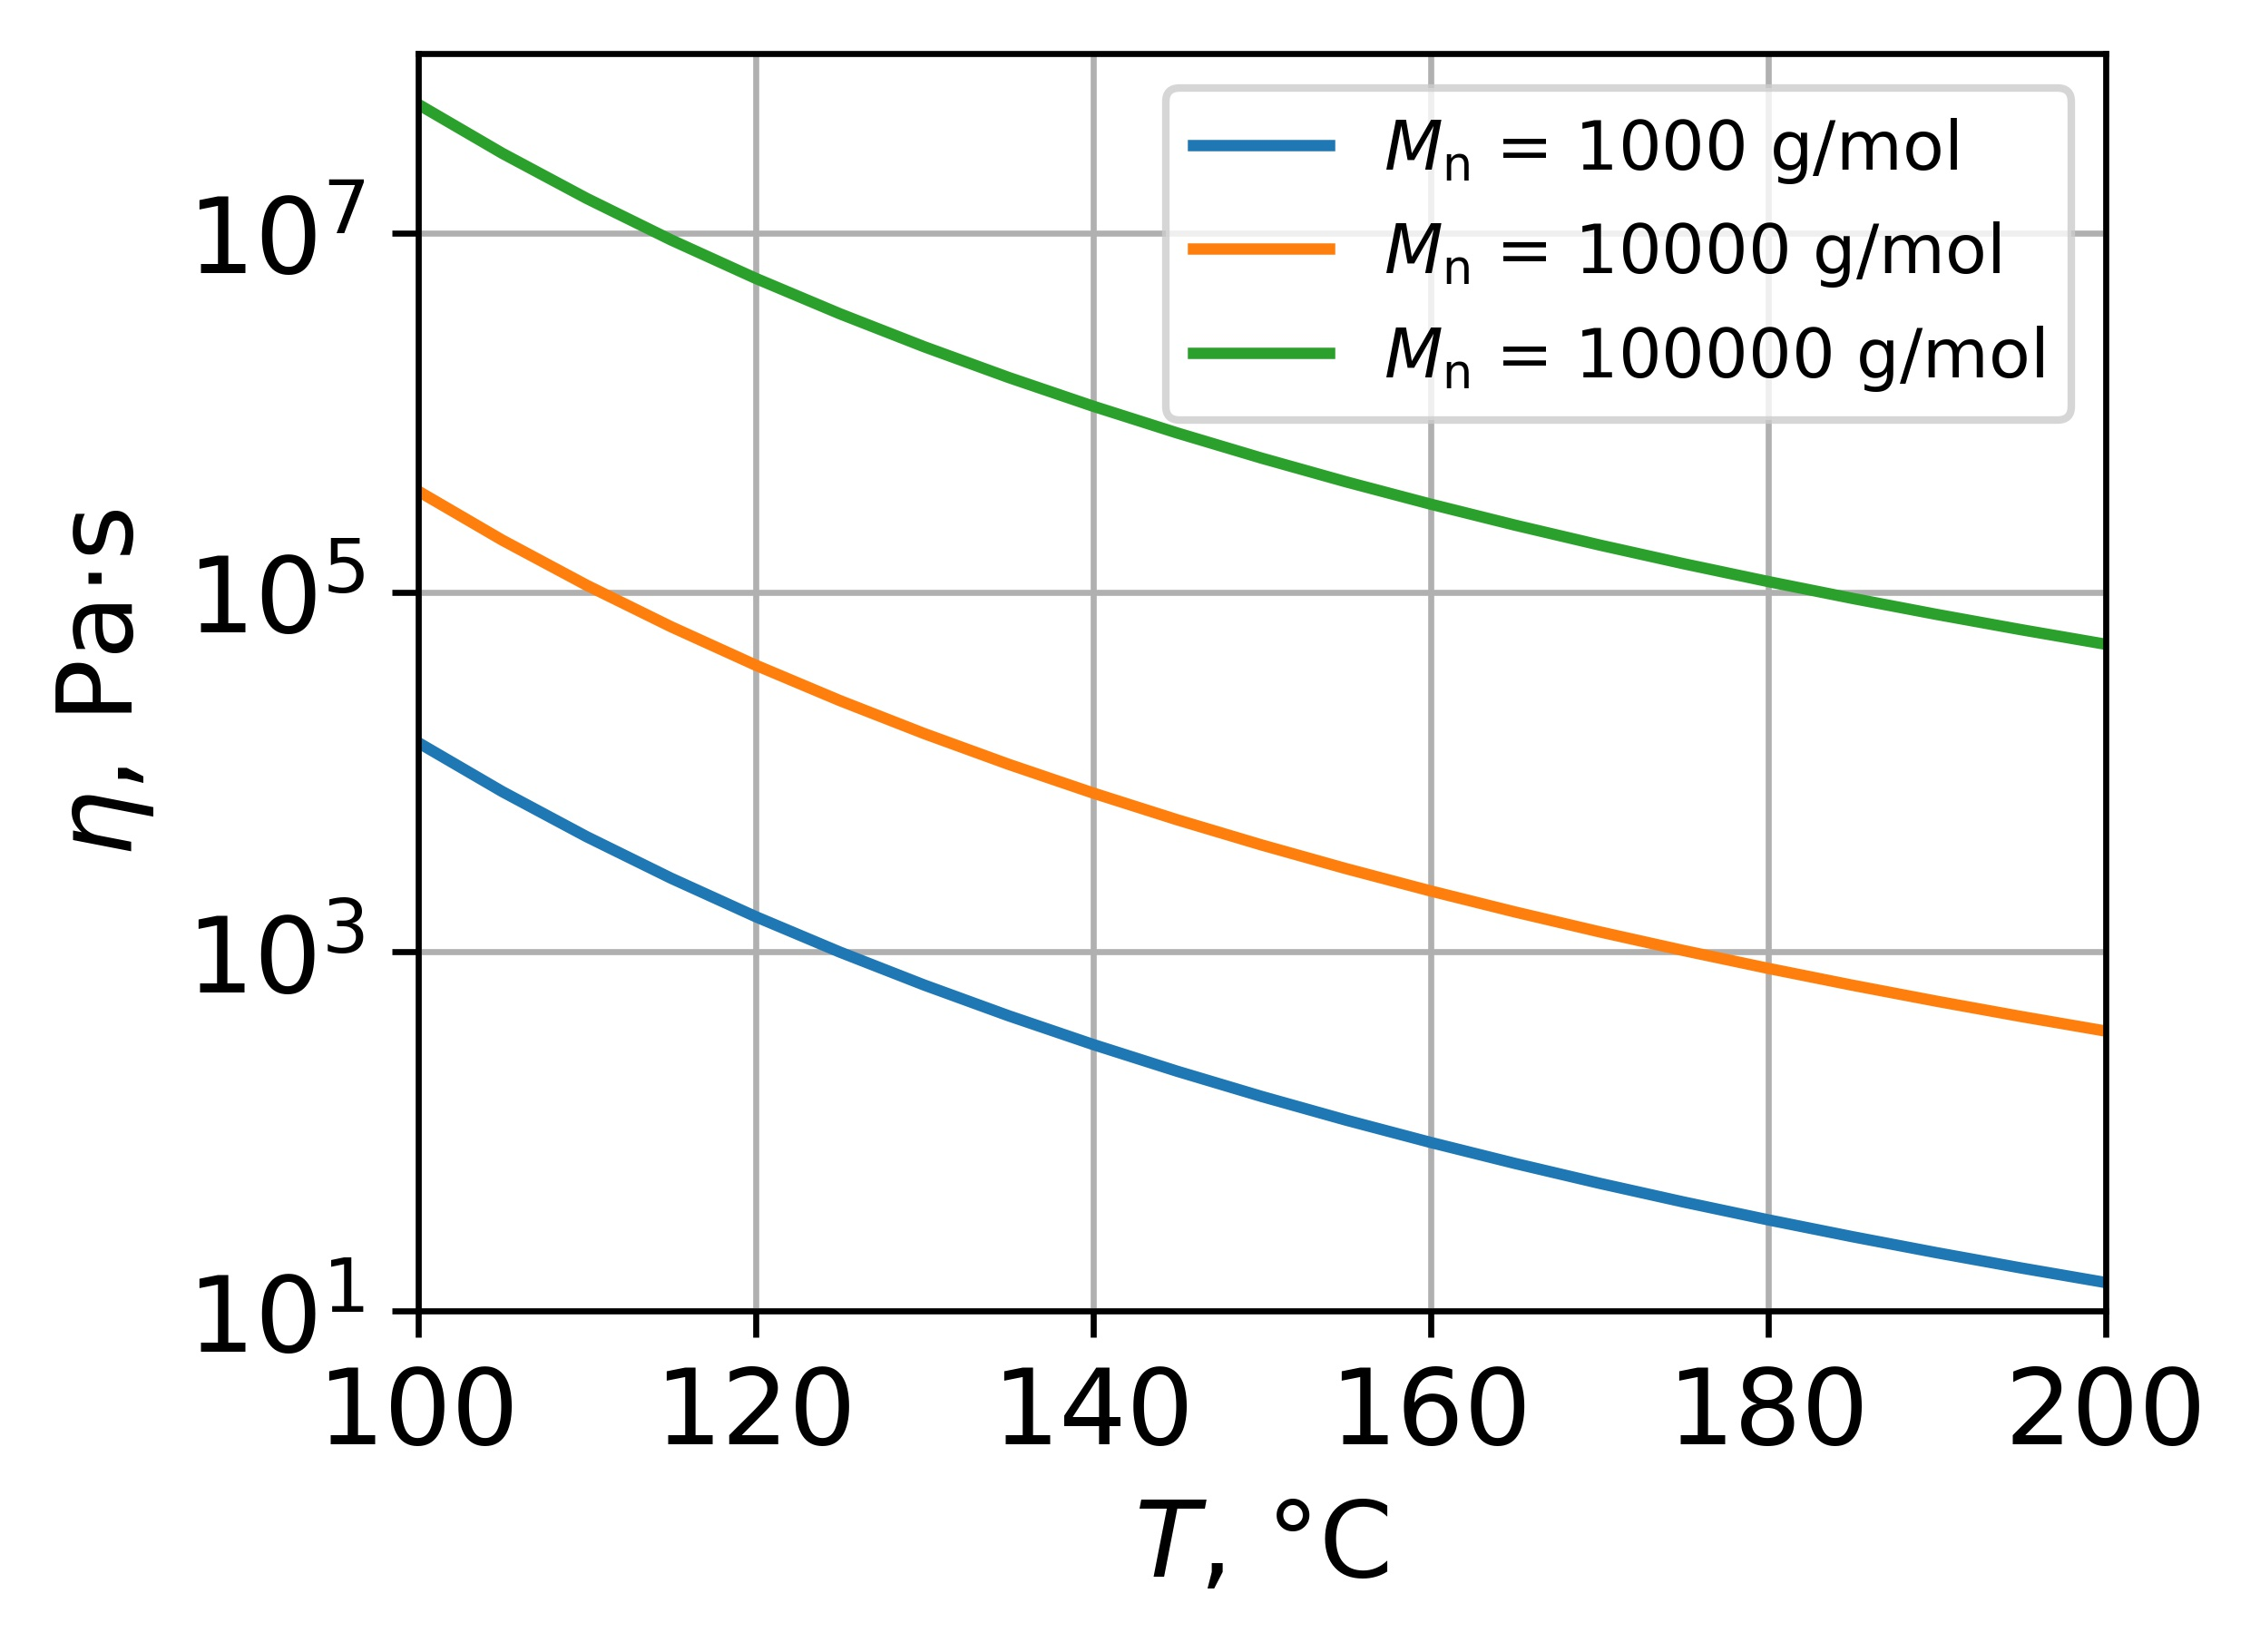
\includegraphics[width=0.6\linewidth]{eta_vary_T_Mn}
	\end{center}
	
	\vspace{-2em}
	
	\caption{Промоделированные периодические профили с периодом 3 мкм, полученные в слое ПММА с начальной толщиной 500 нм методом СЭЛТР при экспонировании по области с различным распределением плотности тока в пучке. Темпера}
	\label{fig:DEBER_multibeam}
\end{figure}


\begin{figure}[t]
	\begin{center}
		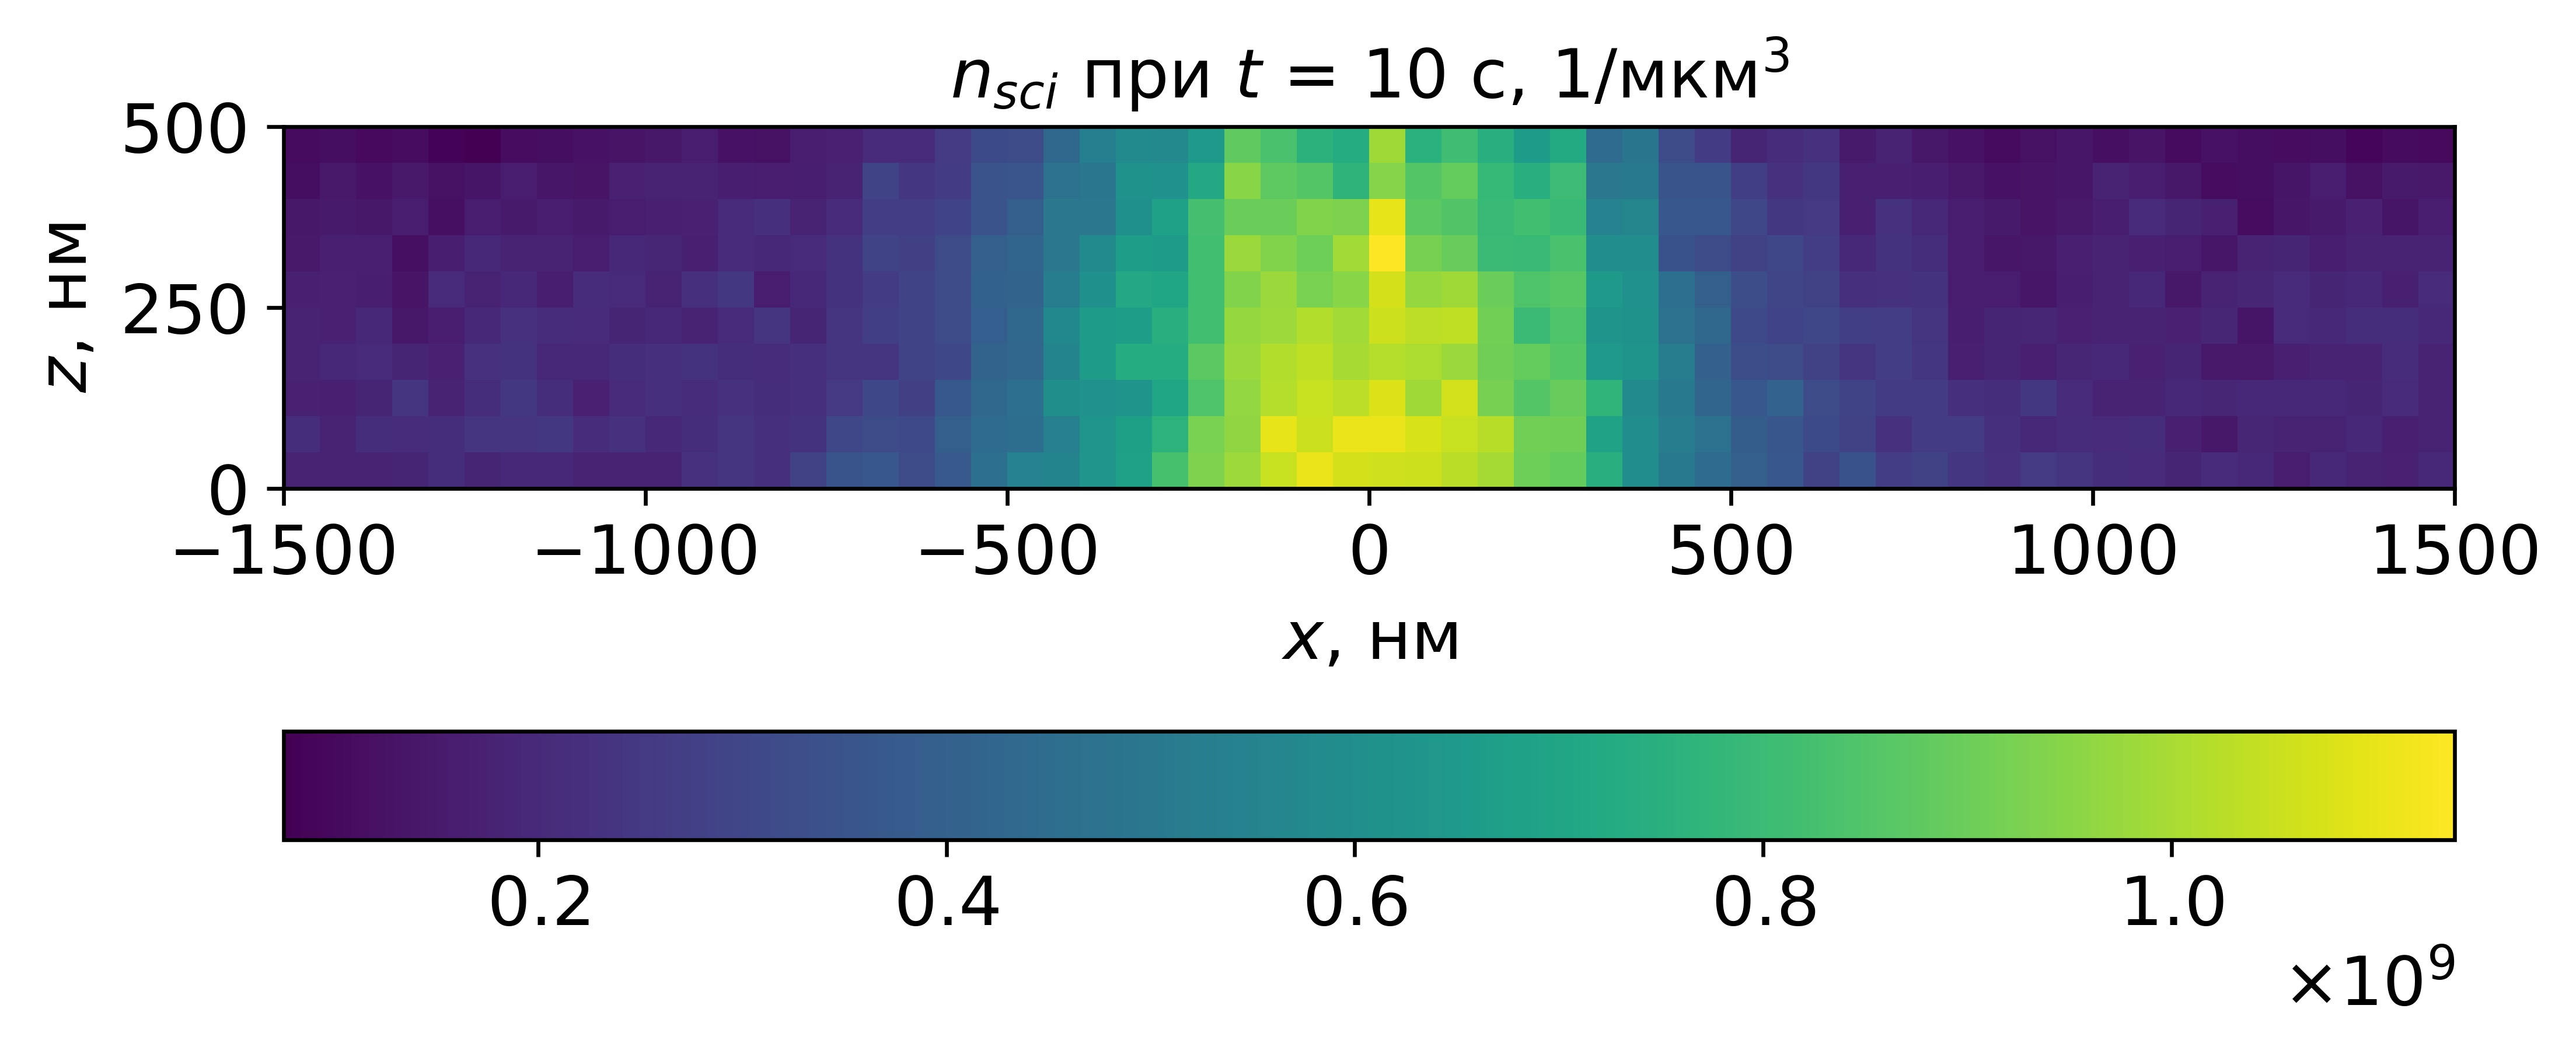
\includegraphics[width=0.7\linewidth]{sci_conc_10s_14} \\
		\vspace{-3.7em} \text{\hspace{-26em} a)} \vspace{2.7em} \\
		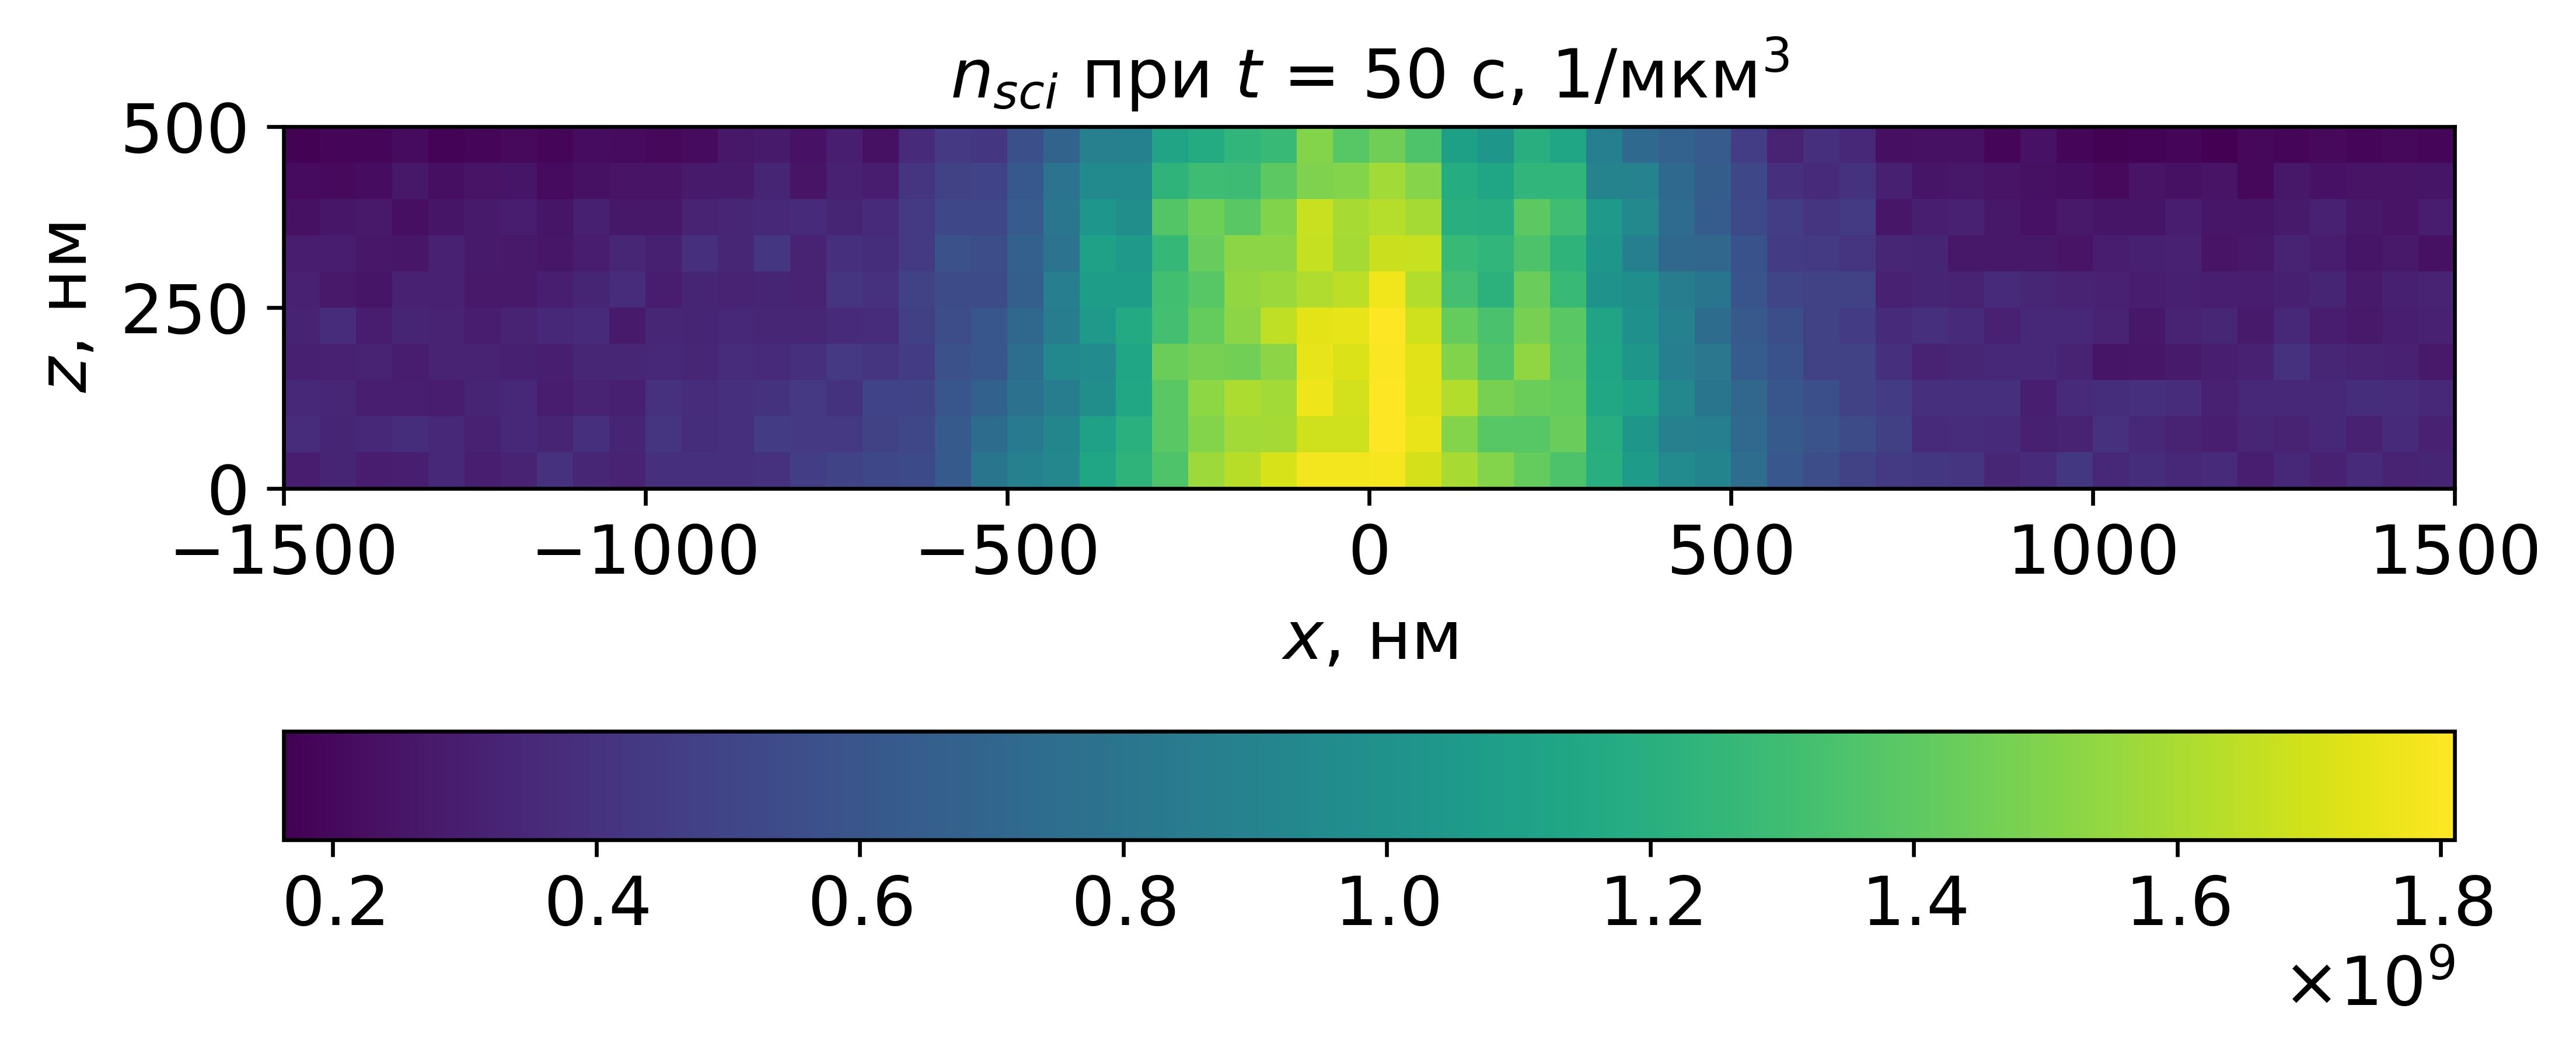
\includegraphics[width=0.7\linewidth]{sci_conc_50s_14} \\
		\vspace{-3.7em} \text{\hspace{-26em} б)} \vspace{3.7em} \\
	\end{center}
	\vspace{-2.5em}
	\caption{Моделирование распределения среднечисловой молекулярной массы ПММА марки 950К при его экспонировании электронным лучом «в кадр», с расстоянием между линиями 3 мкм. На рис. показано распределение локальной молекулярной массы резиста в пределах одной линии. Плотность тока на единицу длины линии составляет около 3 нА/см, начальная энергия электронов в пучке – 20 кэВ, толщина слоя ПММА -- 500 нм, температура образца -- 150 $^\circ$C. Время экспонирования составляет 10 с (а) и 50 с (б).}
	\label{fig:Mn_hist}
\end{figure}

\begin{figure}[t]
	\begin{center}
		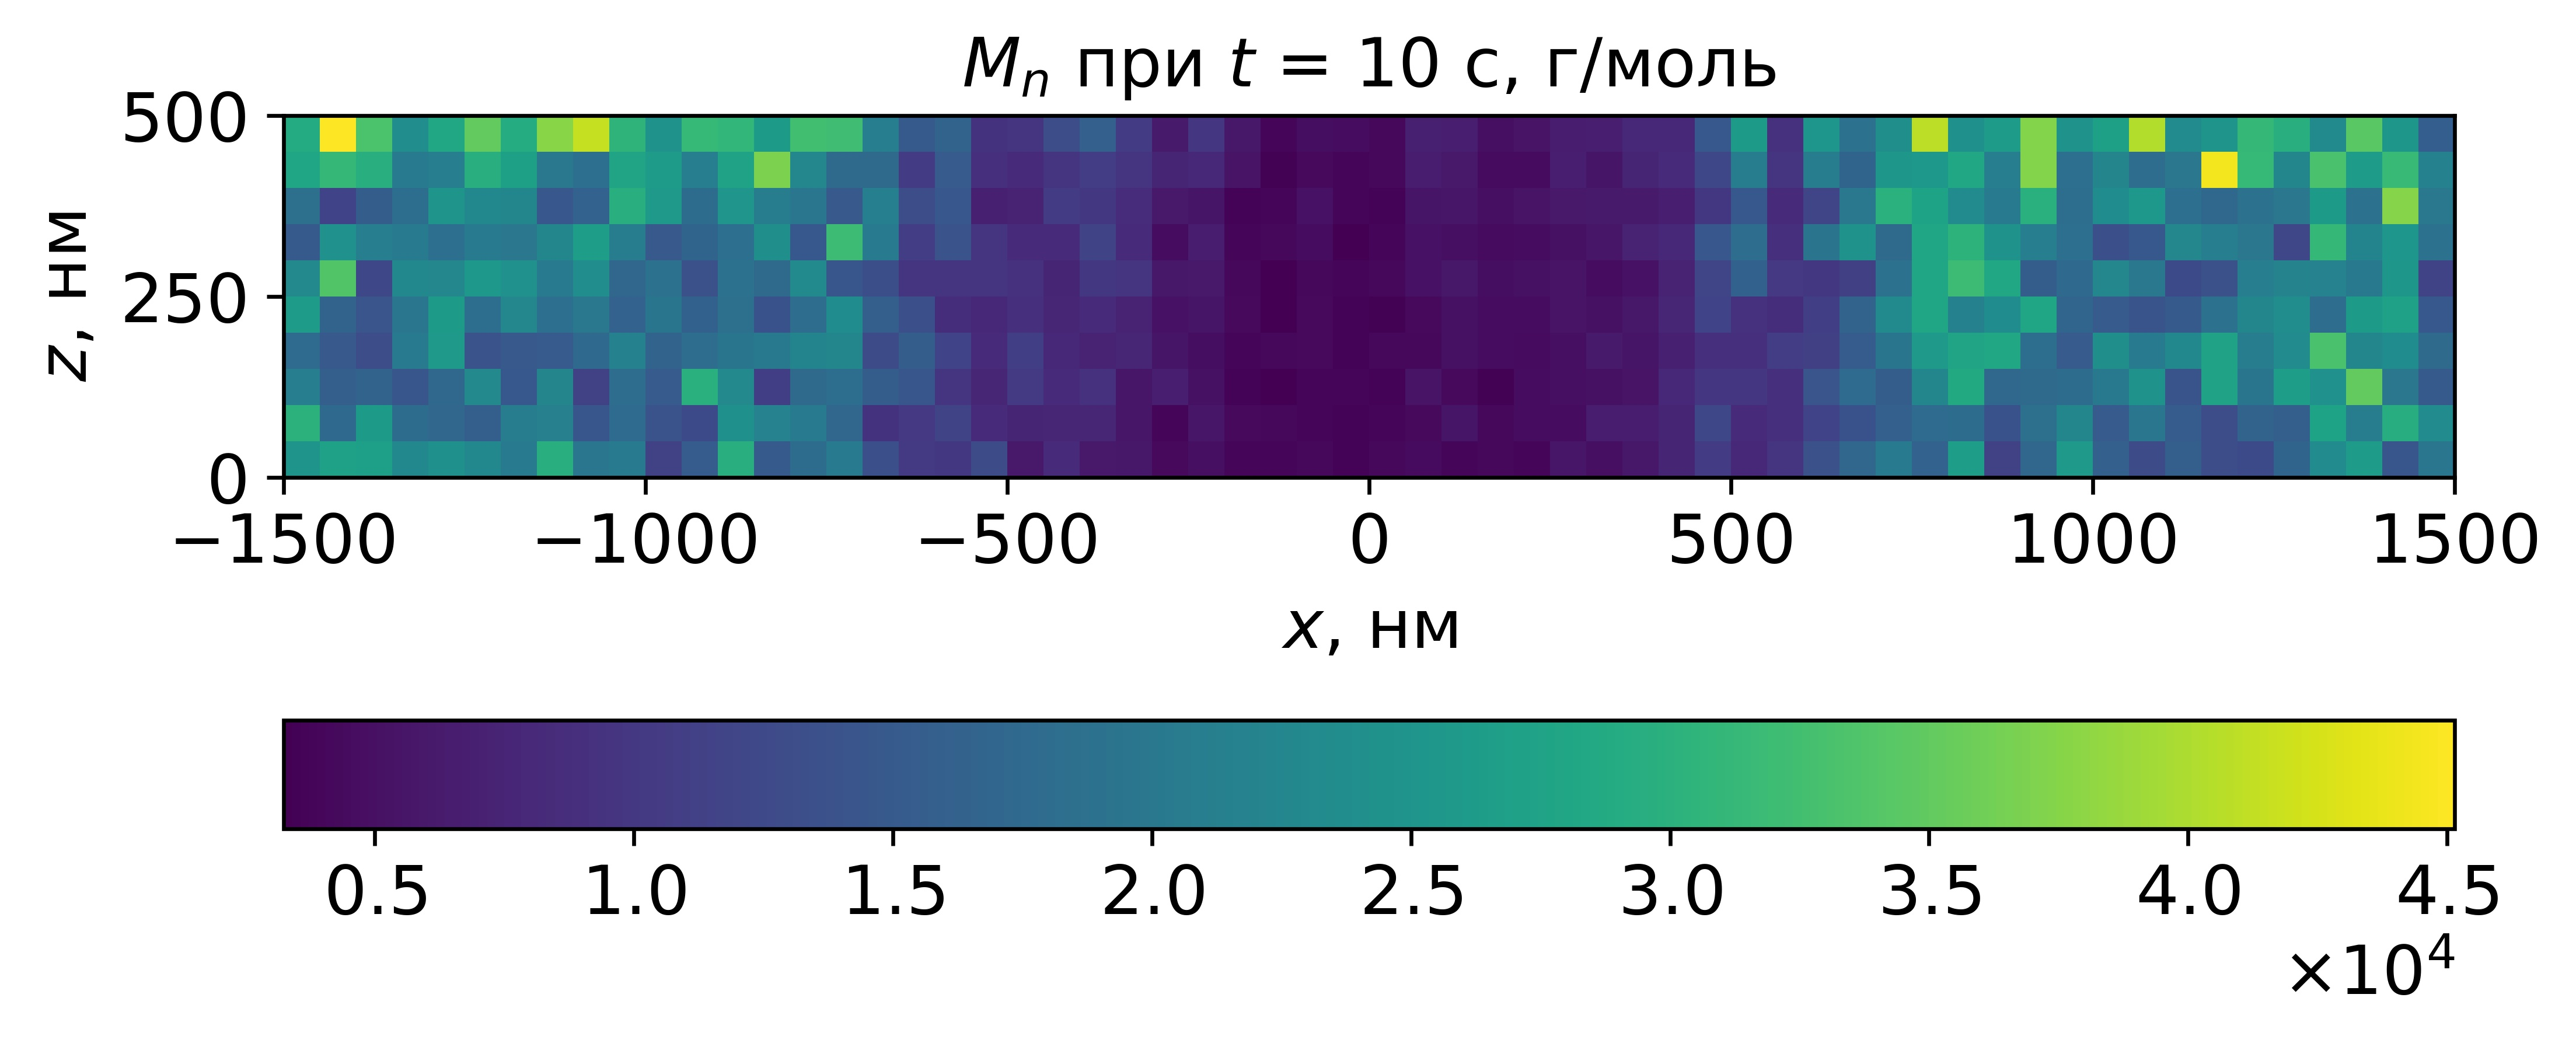
\includegraphics[width=0.7\linewidth]{Mn_hist_10s_14} \\
		\vspace{-3.7em} \text{\hspace{-26em} a)} \vspace{2.7em} \\
		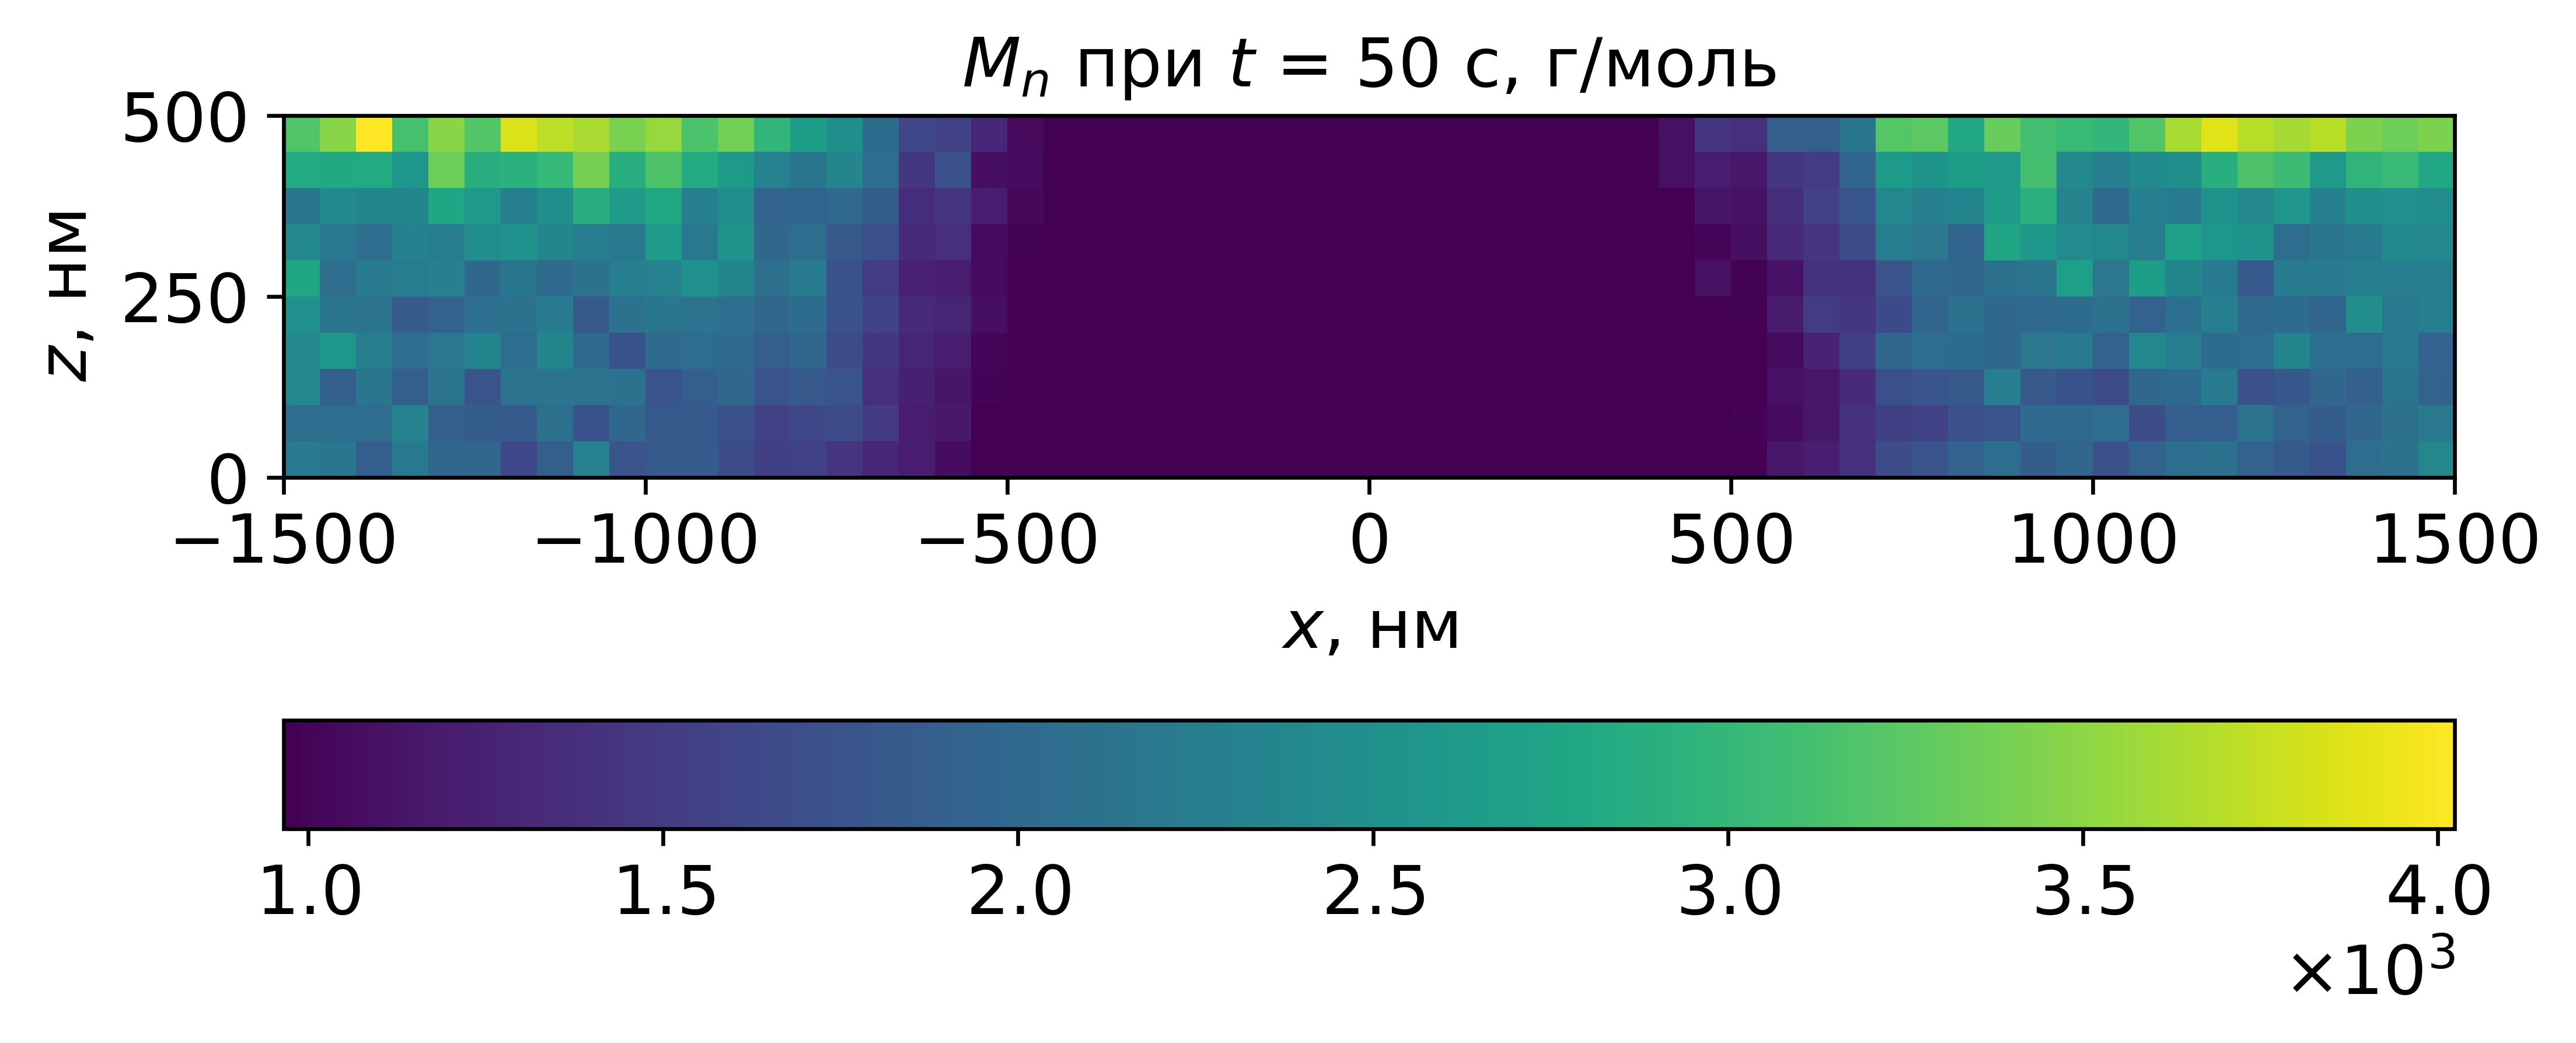
\includegraphics[width=0.7\linewidth]{Mn_hist_50s_14} \\
		\vspace{-3.7em} \text{\hspace{-26em} б)} \vspace{3.7em} \\
	\end{center}
	\vspace{-2.5em}
	\caption{Моделирование распределения среднечисловой молекулярной массы ПММА марки 950К при его экспонировании электронным лучом «в кадр», с расстоянием между линиями 3 мкм. На рис. показано распределение локальной молекулярной массы резиста в пределах одной линии. Плотность тока на единицу длины линии составляет около 3 нА/см, начальная энергия электронов в пучке – 20 кэВ, толщина слоя ПММА -- 500 нм, температура образца -- 150 $^\circ$C. Время экспонирования составляет 10 с (а) и 50 с (б).}
	\label{fig:Mn_hist}
\end{figure}



Учет всех процессов, приводящих к изменению $P_n$ и $R_n$, позволяет описать весь полимерный образец системой уравнений, описывающих каждую степень полимеризации:

\begin{equation}
	\left\{
	\begin{aligned}
		&\dots \\
		&\frac{d P_n}{d t}=-(n-1)(k_S+k_I R / V) P_n-k_E P_n+k_I R / V \sum_{j=n+1}^{\infty} P_j+k_I R_n \frac{d_0}{m_0}+k_T \alpha_n \\
		&\dots \\
		&\frac{d R_n}{d t}=(2 k_S+k_I R / V) \sum_{j=n+1}^{\infty} P_j+k_E P_n-(\frac{k_I d_0}{m_0}+k_P+k_T \beta) R_n+R_P R_{n+1} \\
		&\dots \\
		&\frac{d R_1}{d t}=(2 k_S+k_I R / V) \frac{W}{x m_0}+\frac{k_E}{m_0} \frac{W}{x}-(\frac{k_I d_0}{m_0}+k_T \beta) R_1+k_P R_2,
	\end{aligned}
	\right.
\end{equation}
где $m_0$ -- масса мономера, $x$ -- среднечисловая степень полимеризации образца. 

\begin{equation} \label{eq:Boyd_system_3}
	\left\{
	\begin{aligned}
		&\dots \\
		&d P_n / d t=-(n-1) k_s P_n+k_r R_n \bar{R}, \\
		&\dots \\
		&\dots \\
		&d R_n / d t=2 k_s \sum_{j=n+1}^{\infty} P_j+k_p(R_{n+1}-R_n)-k_T \bar{R} R_n=0 \quad(n \geq 2) \\
		&\dots \\
		&d R_1 / d t=2 k_s(W / x m_0)+k_p R_2-k_T \bar{R} R_1=0
	\end{aligned}
	\right.,
\end{equation}
где $\bar{R} = R/V$.

\begin{equation} \label{eq:moment_equation}
	\frac{d M_i}{d t}=k_s(\frac{2}{i+1}-1) M_{i+1}+\frac{d M_0}{d t}-k_s M_1 - \frac{i}{\gamma}(k_s M_i+\frac{d M_{i-1}}{d t}) \quad(i \geq 1),
\end{equation}
где $1/\gamma = k_p / (k_T \bar{R})$ -- средняя длина цепи деполимеризации, $M_i$ -- момент функции распределения порядка $i$:
\begin{equation}
	M_i=\sum_{n=2}^{\infty} n^i P_n.
\end{equation}

При этом моменты функции распределения высших порядков могут быть выражены через параметры $y$ и $z$ и момент первого порядка $M_1$:
\begin{equation}
	M_i=M_1 \prod_{n=2}^i(z+n) y^{i-1}.
\end{equation}
Отметим, что $M_0$ выражает полное число полимерных молекул, $M_1$ -- среднечисловую степень полимеризации.

Далее удобно ввести безразмерные переменные:
\begin{equation} \label{eq:dim_less_MW}
	\begin{aligned}
		\tau & = y_0 k_s t \\
		\tilde{M}_1 & = M_1 / M_{1_0} \\
		\tilde{y} & = y / y_0 \\
		\tilde{\gamma} & = \gamma y_0 \\
		\tilde{x} & = x / x_0 = \left[y(z+1) / y_0(z_0+1)\right],
	\end{aligned}
\end{equation}
которые в дальнейшем используются в уравнениях вида~\ref{eq:moment_equation} для $i$, равного 1, 2 и 3 (величины с нижним индексом ``0'' соответствуют начальному состоянию).


\begin{equation}
\begin{aligned}
\frac{M^{0}_{1}}{\gamma (z(t) + 1)^{2} \tilde{y}^{2}(t)}
\left[ - \gamma y_{0} (z(t) + 1)^{2} \tilde{y}^{2}(t) \frac{d}{d t} \tilde{M_1}(t) \right. (z(t) + 1)^{2} \tilde{M_1}(t) \tilde{y}^{2}(t) & - \\
 + (z(t) + 1) \tilde{M_1}(t) \frac{d}{d t} \tilde{y}(t) -
\left. (z(t) + 1) \tilde{y}(t) \frac{d}{d t} \tilde{M_1}(t) + \tilde{M_1}(t) \tilde{y}(t) \frac{d}{d t} z(t) \right] & = 0
\end{aligned}
\end{equation}


\begin{equation}
\begin{aligned}
- \frac{M^{0}_{1} y_{0}}{3 \gamma}
\left[\gamma y_{0} \left(\left(z{\left(t \right)} + 2\right) \left(z{\left(t \right)} + 3\right) \tilde{M_1}{\left(t \right)} \tilde{y}^{2}{\left(t \right)} + 3 \left(z{\left(t \right)} + 2\right) \tilde{M_1}{\left(t \right)} \frac{d}{d t} \tilde{y}{\left(t \right)} \right. \right. & + \\
\left. \left. 3 \left(z{\left(t \right)} + 2\right) \tilde{y}{\left(t \right)} \frac{d}{d t} \tilde{M_1}{\left(t \right)} + 3 \tilde{M_1}{\left(t \right)} \tilde{y}{\left(t \right)} \frac{d}{d t} z{\left(t \right)}\right) + 6 \left(z{\left(t \right)} + 2\right) \tilde{M_1}{\left(t \right)} \tilde{y}{\left(t \right)} + 6 \frac{d}{d t} \tilde{M_1}{\left(t \right)}\right] & = 0
\end{aligned}
\end{equation}


\begin{equation}
\begin{aligned}
- \frac{M^{0}_{1} y_{0}^{2}}{2 \gamma} \left[\gamma y_{0} \left(\left(z{\left(t \right)} + 2\right) \left(z{\left(t \right)} + 3\right) \left(z{\left(t \right)} + 4\right) \tilde{M_1}{\left(t \right)} \tilde{y}^{2}{\left(t \right)} \right. \right. & + \\
\left. \left.  4 \left(z{\left(t \right)} + 2\right) \left(z{\left(t \right)} + 3\right) \tilde{M_1}{\left(t \right)} \frac{d}{d t} \tilde{y}{\left(t \right)} \right. \right. & + \\
\left. \left. 2 \left(z{\left(t \right)} + 2\right) \left(z{\left(t \right)} + 3\right) \tilde{y}{\left(t \right)} \frac{d}{d t} \tilde{M_1}{\left(t \right)} + 2 \left(z{\left(t \right)} + 2\right) \tilde{M_1}{\left(t \right)} \tilde{y}{\left(t \right)} \frac{d}{d t} z{\left(t \right)} \right. \right. & + \\
\left. \left. 2 \left(z{\left(t \right)} + 3\right) \tilde{M_1}{\left(t \right)} \tilde{y}{\left(t \right)} \frac{d}{d t} z{\left(t \right)}\right) \tilde{y}{\left(t \right)} \right. & + \\
\left. 6 \left(z{\left(t \right)} + 2\right) \left(z{\left(t \right)} + 3\right) \tilde{M_1}{\left(t \right)} \tilde{y}^{2}{\left(t \right)} + 6 \left(z{\left(t \right)} + 2\right) \tilde{M_1}{\left(t \right)} \frac{d}{d t} \tilde{y}{\left(t \right)} \right. & + \\
\left. 6 \left(z{\left(t \right)} + 2\right) \tilde{y}{\left(t \right)} \frac{d}{d t} \tilde{M_1}{\left(t \right)} + 6 \tilde{M_1}{\left(t \right)} \tilde{y}{\left(t \right)} \frac{d}{d t} z{\left(t \right)}\right] & = 0
\end{aligned}
\end{equation}


Выражение для 1 производной:
\begin{equation}
\frac{d \tilde{M_1}(t)}{d \tau} = - \tilde{M_1}(t) \tilde{y}(t) \frac{A}{B}
\end{equation}

\begin{equation}
	\begin{aligned}
		A = 9 \gamma^{2} \left(y^{0}\right)^{2} \tilde{y}^{2}{\left(t \right)} z^{3}{\left(t \right)} + 41 \gamma^{2} \left(y^{0}\right)^{2} \tilde{y}^{2}{\left(t \right)} z^{2}{\left(t \right)} + 58 \gamma^{2} \left(y^{0}\right)^{2} \tilde{y}^{2}{\left(t \right)} z{\left(t \right)} + \\
		24 \gamma^{2} \left(y^{0}\right)^{2} \tilde{y}^{2}{\left(t \right)} + 24 \gamma y^{0} \tilde{y}{\left(t \right)} z^{2}{\left(t \right)} + 96 \gamma y^{0} \tilde{y}{\left(t \right)} z{\left(t \right)} + 96 \gamma y^{0} \tilde{y}{\left(t \right)} + 36 z{\left(t \right)} + 72 \\
	\end{aligned}
\end{equation}

\begin{equation}
	\begin{aligned}
		B = 6 \gamma^{3} \left(y^{0}\right)^{3} \tilde{y}^{3}{\left(t \right)} z^{3}{\left(t \right)} + 24 \gamma^{3} \left(y^{0}\right)^{3} \tilde{y}^{3}{\left(t \right)} z^{2}{\left(t \right)} + 30 \gamma^{3} \left(y^{0}\right)^{3} \tilde{y}^{3}{\left(t \right)} z{\left(t \right)} + \\
		12 \gamma^{3} \left(y^{0}\right)^{3} \tilde{y}^{3}{\left(t \right)} + 18 \gamma^{2} \left(y^{0}\right)^{2} \tilde{y}^{2}{\left(t \right)} z^{2}{\left(t \right)} + \\
		66 \gamma^{2} \left(y^{0}\right)^{2} \tilde{y}^{2}{\left(t \right)} z{\left(t \right)} + 60 \gamma^{2} \left(y^{0}\right)^{2} \tilde{y}^{2}{\left(t \right)} + 36 \gamma y^{0} \tilde{y}{\left(t \right)} z{\left(t \right)} + 84 \gamma y^{0} \tilde{y}{\left(t \right)} + 36
	\end{aligned}
\end{equation}


Выражение для 2 производной:
\begin{equation}
	\frac{d \tilde{y}(t)}{d \tau} = \tilde{y}^{2}{\left(t \right)} \frac{C}{6 D}
\end{equation}

\begin{equation}
	\begin{aligned}
		C = \gamma^{3} \left(y^{0}\right)^{3} \tilde{y}^{3}{\left(t \right)} z^{5}{\left(t \right)} + 5 \gamma^{3} \left(y^{0}\right)^{3} \tilde{y}^{3}{\left(t \right)} z^{4}{\left(t \right)} + 3 \gamma^{3} \left(y^{0}\right)^{3} \tilde{y}^{3}{\left(t \right)} z^{3}{\left(t \right)} - \\
		17 \gamma^{3} \left(y^{0}\right)^{3} \tilde{y}^{3}{\left(t \right)} z^{2}{\left(t \right)} - 28 \gamma^{3} \left(y^{0}\right)^{3} \tilde{y}^{3}{\left(t \right)} z{\left(t \right)} - 12 \gamma^{3} \left(y^{0}\right)^{3} \tilde{y}^{3}{\left(t \right)} + \\
		6 \gamma^{2} \left(y^{0}\right)^{2} \tilde{y}^{2}{\left(t \right)} z^{4}{\left(t \right)} + 27 \gamma^{2} \left(y^{0}\right)^{2} \tilde{y}^{2}{\left(t \right)} z^{3}{\left(t \right)} + 19 \gamma^{2} \left(y^{0}\right)^{2} \tilde{y}^{2}{\left(t \right)} z^{2}{\left(t \right)} - \\
		52 \gamma^{2} \left(y^{0}\right)^{2} \tilde{y}^{2}{\left(t \right)} z{\left(t \right)} - 60 \gamma^{2} \left(y^{0}\right)^{2} \tilde{y}^{2}{\left(t \right)} + 18 \gamma y^{0} \tilde{y}{\left(t \right)} z^{3}{\left(t \right)} + 42 \gamma y^{0} \tilde{y}{\left(t \right)} z^{2}{\left(t \right)} - \\
		24 \gamma y^{0} \tilde{y}{\left(t \right)} z{\left(t \right)} - 84 \gamma y^{0} \tilde{y}{\left(t \right)} - 36
	\end{aligned}
\end{equation}

\begin{equation}
	\begin{aligned}
		D = \gamma^{3} \left(y^{0}\right)^{3} \tilde{y}^{3}{\left(t \right)} z^{3}{\left(t \right)} + 4 \gamma^{3} \left(y^{0}\right)^{3} \tilde{y}^{3}{\left(t \right)} z^{2}{\left(t \right)} + 5 \gamma^{3} \left(y^{0}\right)^{3} \tilde{y}^{3}{\left(t \right)} z{\left(t \right)} + \\
		2 \gamma^{3} \left(y^{0}\right)^{3} \tilde{y}^{3}{\left(t \right)} + 3 \gamma^{2} \left(y^{0}\right)^{2} \tilde{y}^{2}{\left(t \right)} z^{2}{\left(t \right)} + 11 \gamma^{2} \left(y^{0}\right)^{2} \tilde{y}^{2}{\left(t \right)} z{\left(t \right)} + \\
		10 \gamma^{2} \left(y^{0}\right)^{2} \tilde{y}^{2}{\left(t \right)} + 6 \gamma y^{0} \tilde{y}{\left(t \right)} z{\left(t \right)} + 14 \gamma y^{0} \tilde{y}{\left(t \right)} + 6
	\end{aligned}
\end{equation}

Выражения для 3 производной:
\begin{equation}
	\frac{d \tilde{y}(t)}{d \tau} = - \gamma y^{0} \tilde{y}^{2}(t) z(t) \frac{E}{F}
\end{equation}

\begin{equation}
	\begin{aligned}
		E = \gamma^{2} \left(y^{0}\right)^{2} \tilde{y}^{2}{\left(t \right)} z^{5}{\left(t \right)} + 9 \gamma^{2} \left(y^{0}\right)^{2} \tilde{y}^{2}{\left(t \right)} z^{4}{\left(t \right)} + \\
		31 \gamma^{2} \left(y^{0}\right)^{2} \tilde{y}^{2}{\left(t \right)} z^{3}{\left(t \right)} + 51 \gamma^{2} \left(y^{0}\right)^{2} \tilde{y}^{2}{\left(t \right)} z^{2}{\left(t \right)} + \\
		40 \gamma^{2} \left(y^{0}\right)^{2} \tilde{y}^{2}{\left(t \right)} z{\left(t \right)} + 12 \gamma^{2} \left(y^{0}\right)^{2} \tilde{y}^{2}{\left(t \right)} + \\
		6 \gamma y^{0} \tilde{y}{\left(t \right)} z^{4}{\left(t \right)} + 48 \gamma y^{0} \tilde{y}{\left(t \right)} z^{3}{\left(t \right)} + \\
		138 \gamma y^{0} \tilde{y}{\left(t \right)} z^{2}{\left(t \right)} + 168 \gamma y^{0} \tilde{y}{\left(t \right)} z{\left(t \right)} + \\
		72 \gamma y^{0} \tilde{y}{\left(t \right)} + 18 z^{3}{\left(t \right)} + 84 z^{2}{\left(t \right)} + 126 z{\left(t \right)} + 60
	\end{aligned}
\end{equation}

\begin{equation}
	\begin{aligned}
		F = 6 \gamma^{3} \left(y^{0}\right)^{3} \tilde{y}^{3}{\left(t \right)} z^{3}{\left(t \right)} + 24 \gamma^{3} \left(y^{0}\right)^{3} \tilde{y}^{3}{\left(t \right)} z^{2}{\left(t \right)} + \\
		30 \gamma^{3} \left(y^{0}\right)^{3} \tilde{y}^{3}{\left(t \right)} z{\left(t \right)} + 12 \gamma^{3} \left(y^{0}\right)^{3} \tilde{y}^{3}{\left(t \right)} + \\
		18 \gamma^{2} \left(y^{0}\right)^{2} \tilde{y}^{2}{\left(t \right)} z^{2}{\left(t \right)} + 66 \gamma^{2} \left(y^{0}\right)^{2} \tilde{y}^{2}{\left(t \right)} z{\left(t \right)} + \\
		60 \gamma^{2} \left(y^{0}\right)^{2} \tilde{y}^{2}{\left(t \right)} + 36 \gamma y^{0} \tilde{y}{\left(t \right)} z{\left(t \right)} + 84 \gamma y^{0} \tilde{y}{\left(t \right)} + 36
	\end{aligned}
\end{equation}


\begin{figure}
	\begin{center}
		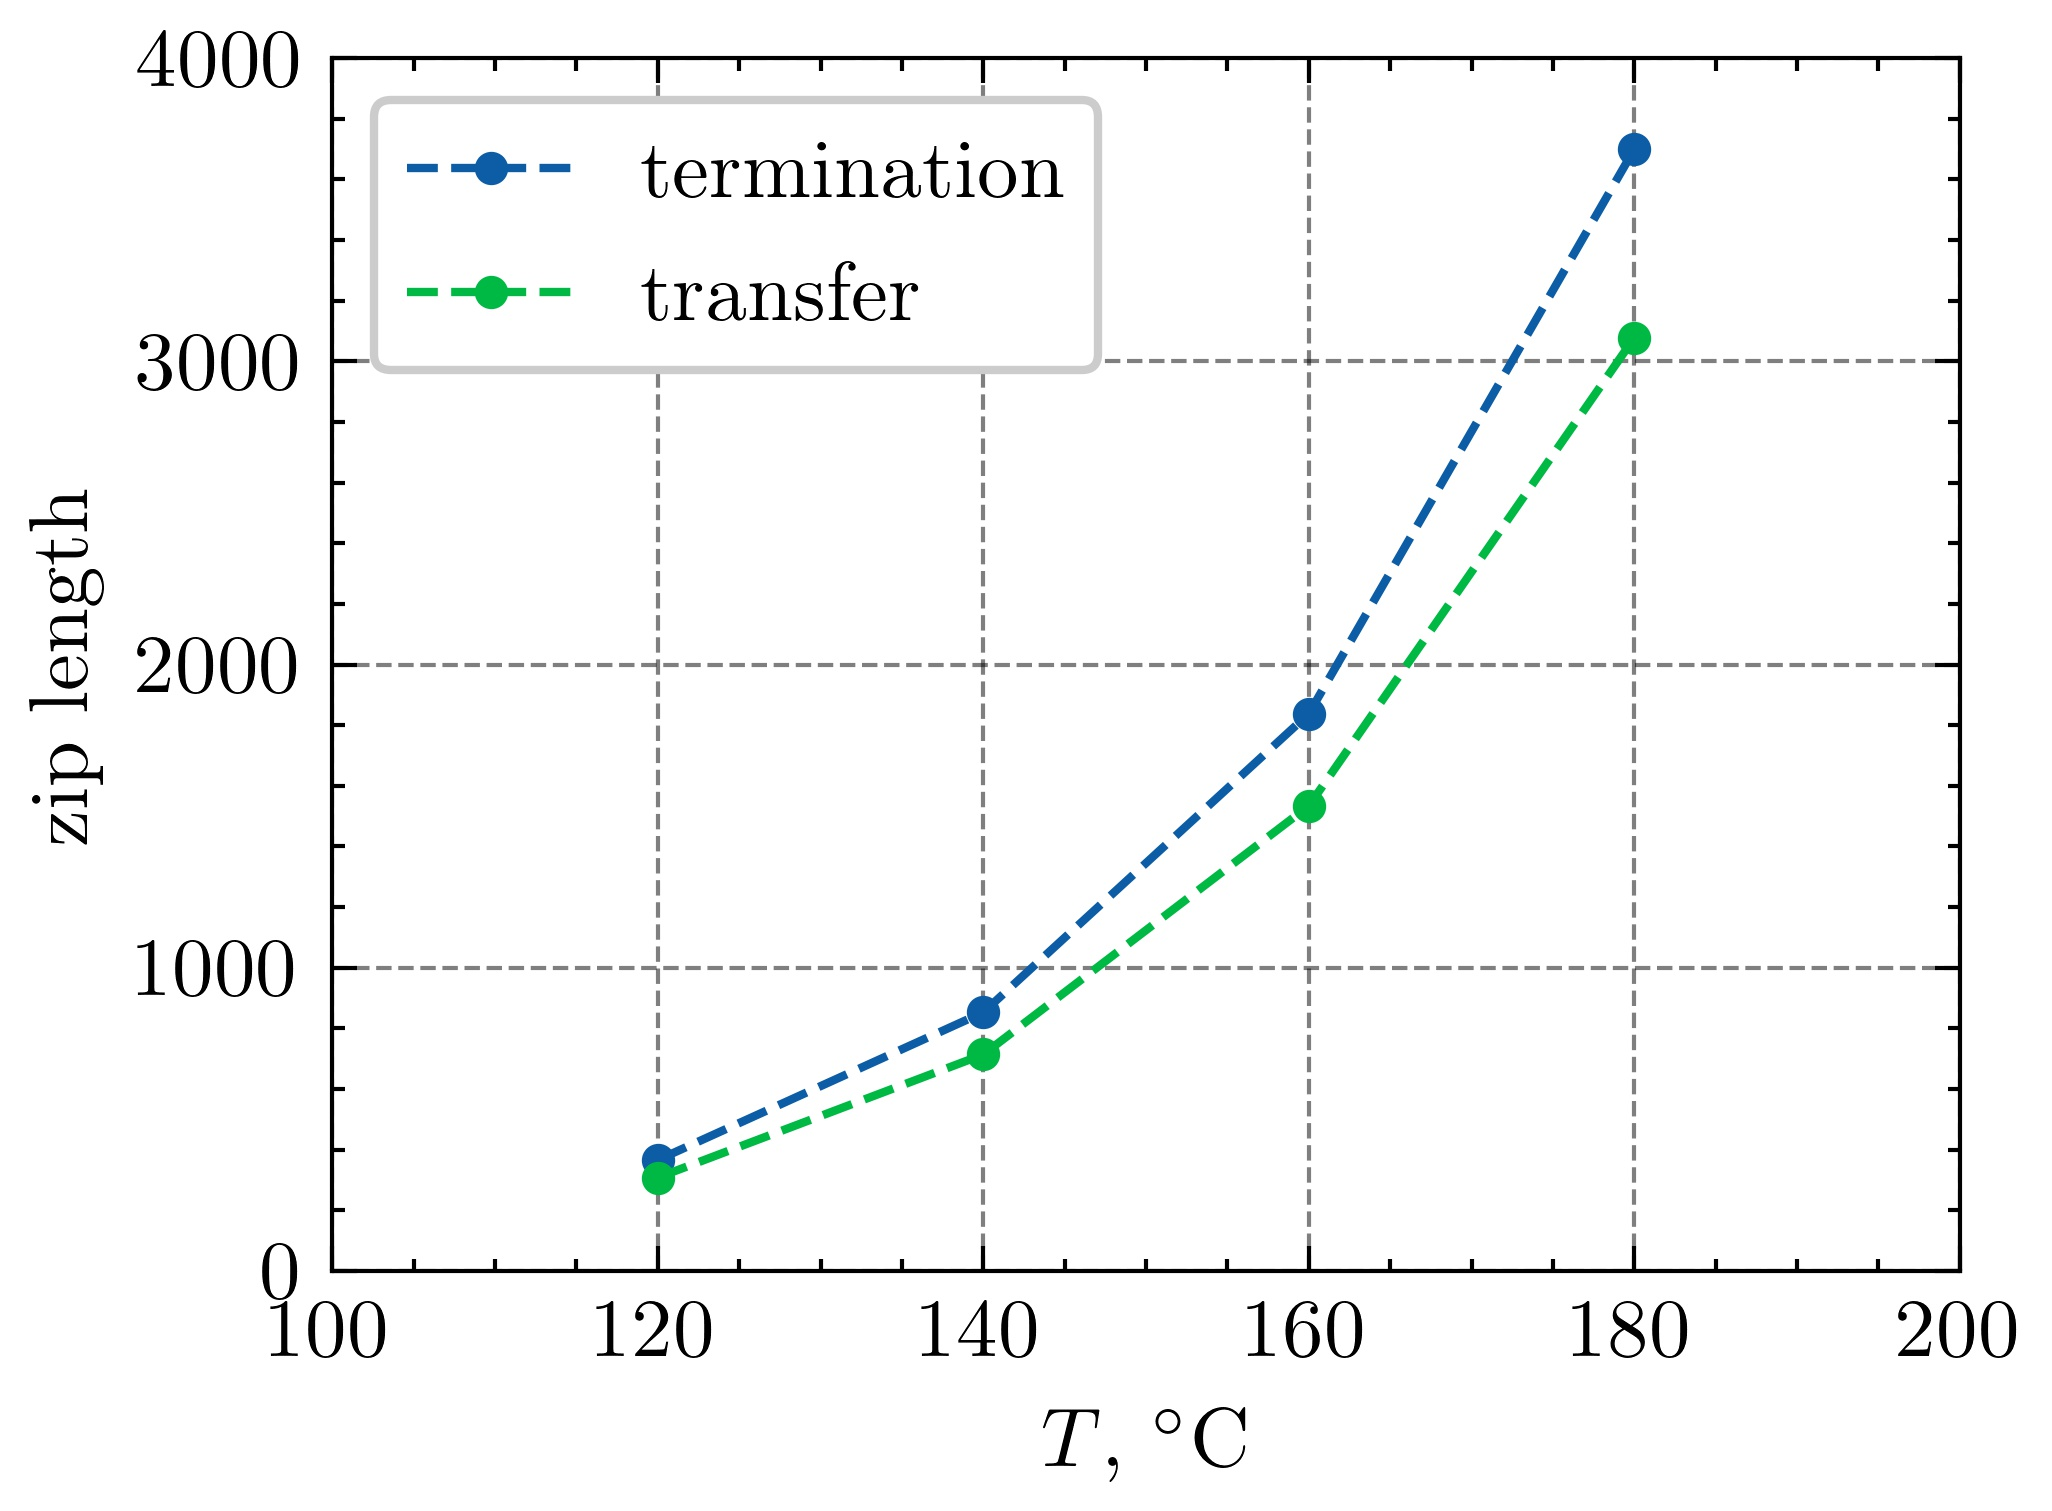
\includegraphics[width=0.6\linewidth]{zip_len_term_trans}
	\end{center}
	
	\vspace{-2em}
	
	\caption{Промоделированные периодические профили с периодом 3 мкм, полученные в слое ПММА с начальной толщиной 500 нм методом СЭЛТР при экспонировании по области с различным распределением плотности тока в пучке. Темпера}
	\label{fig:DEBER_multibeam}
\end{figure}


\begin{figure}
	\begin{minipage}{0.48\textwidth}
		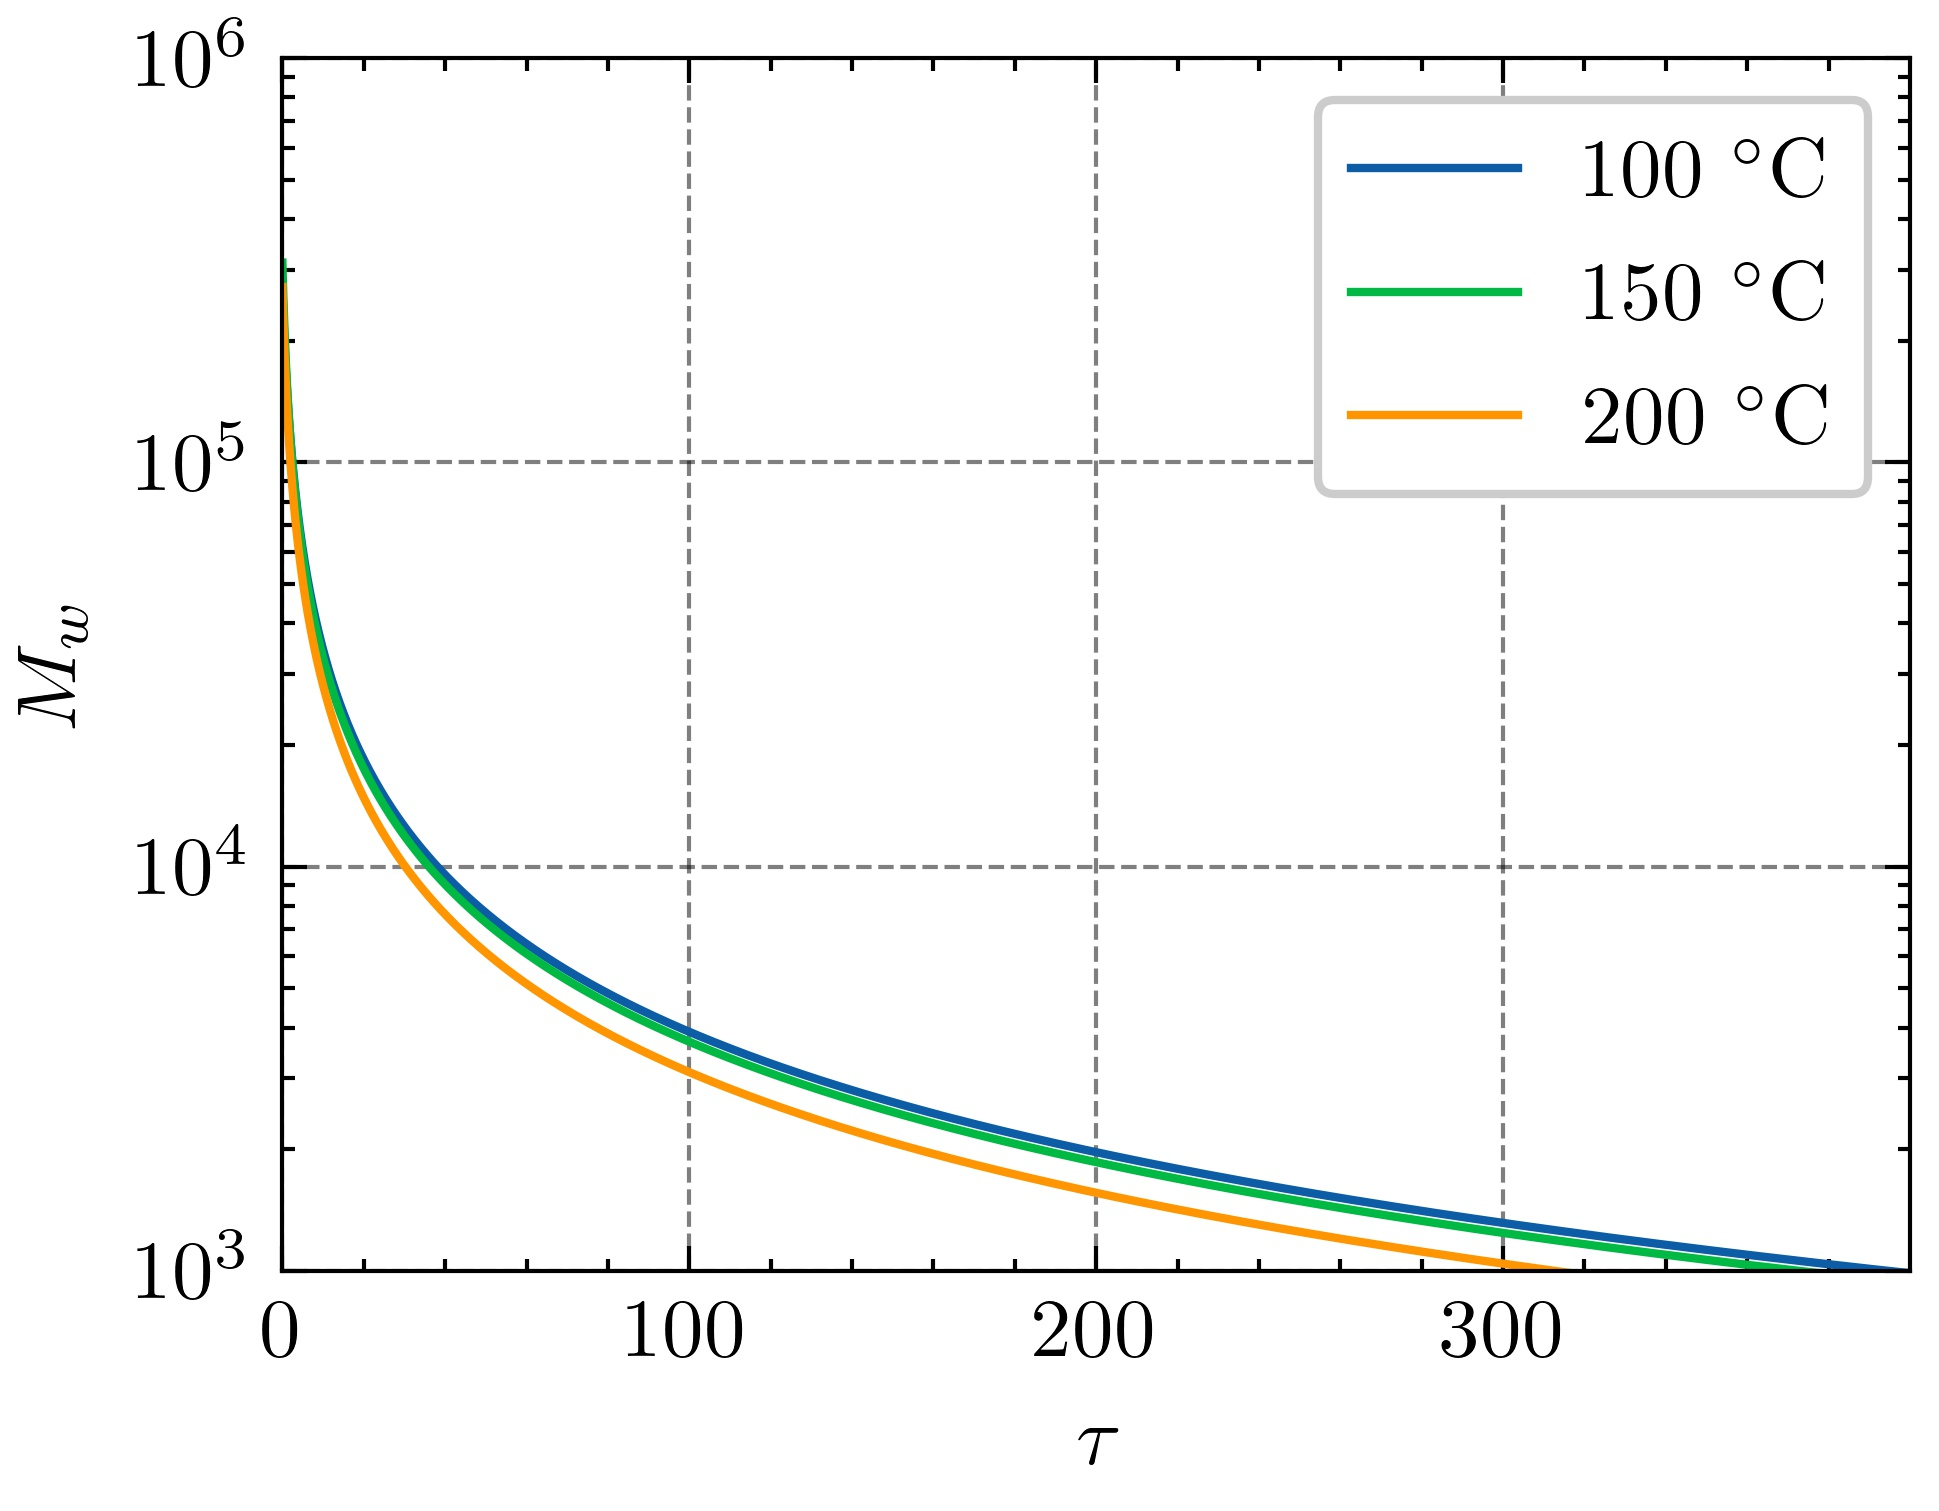
\includegraphics[width=\linewidth]{Mn_tau_100_150_200} \\
		\vspace{-13em} \\ \text{\hspace{0em} a}) \\ \vspace{13em}
	\end{minipage}
	\begin{minipage}{0.48\textwidth}
		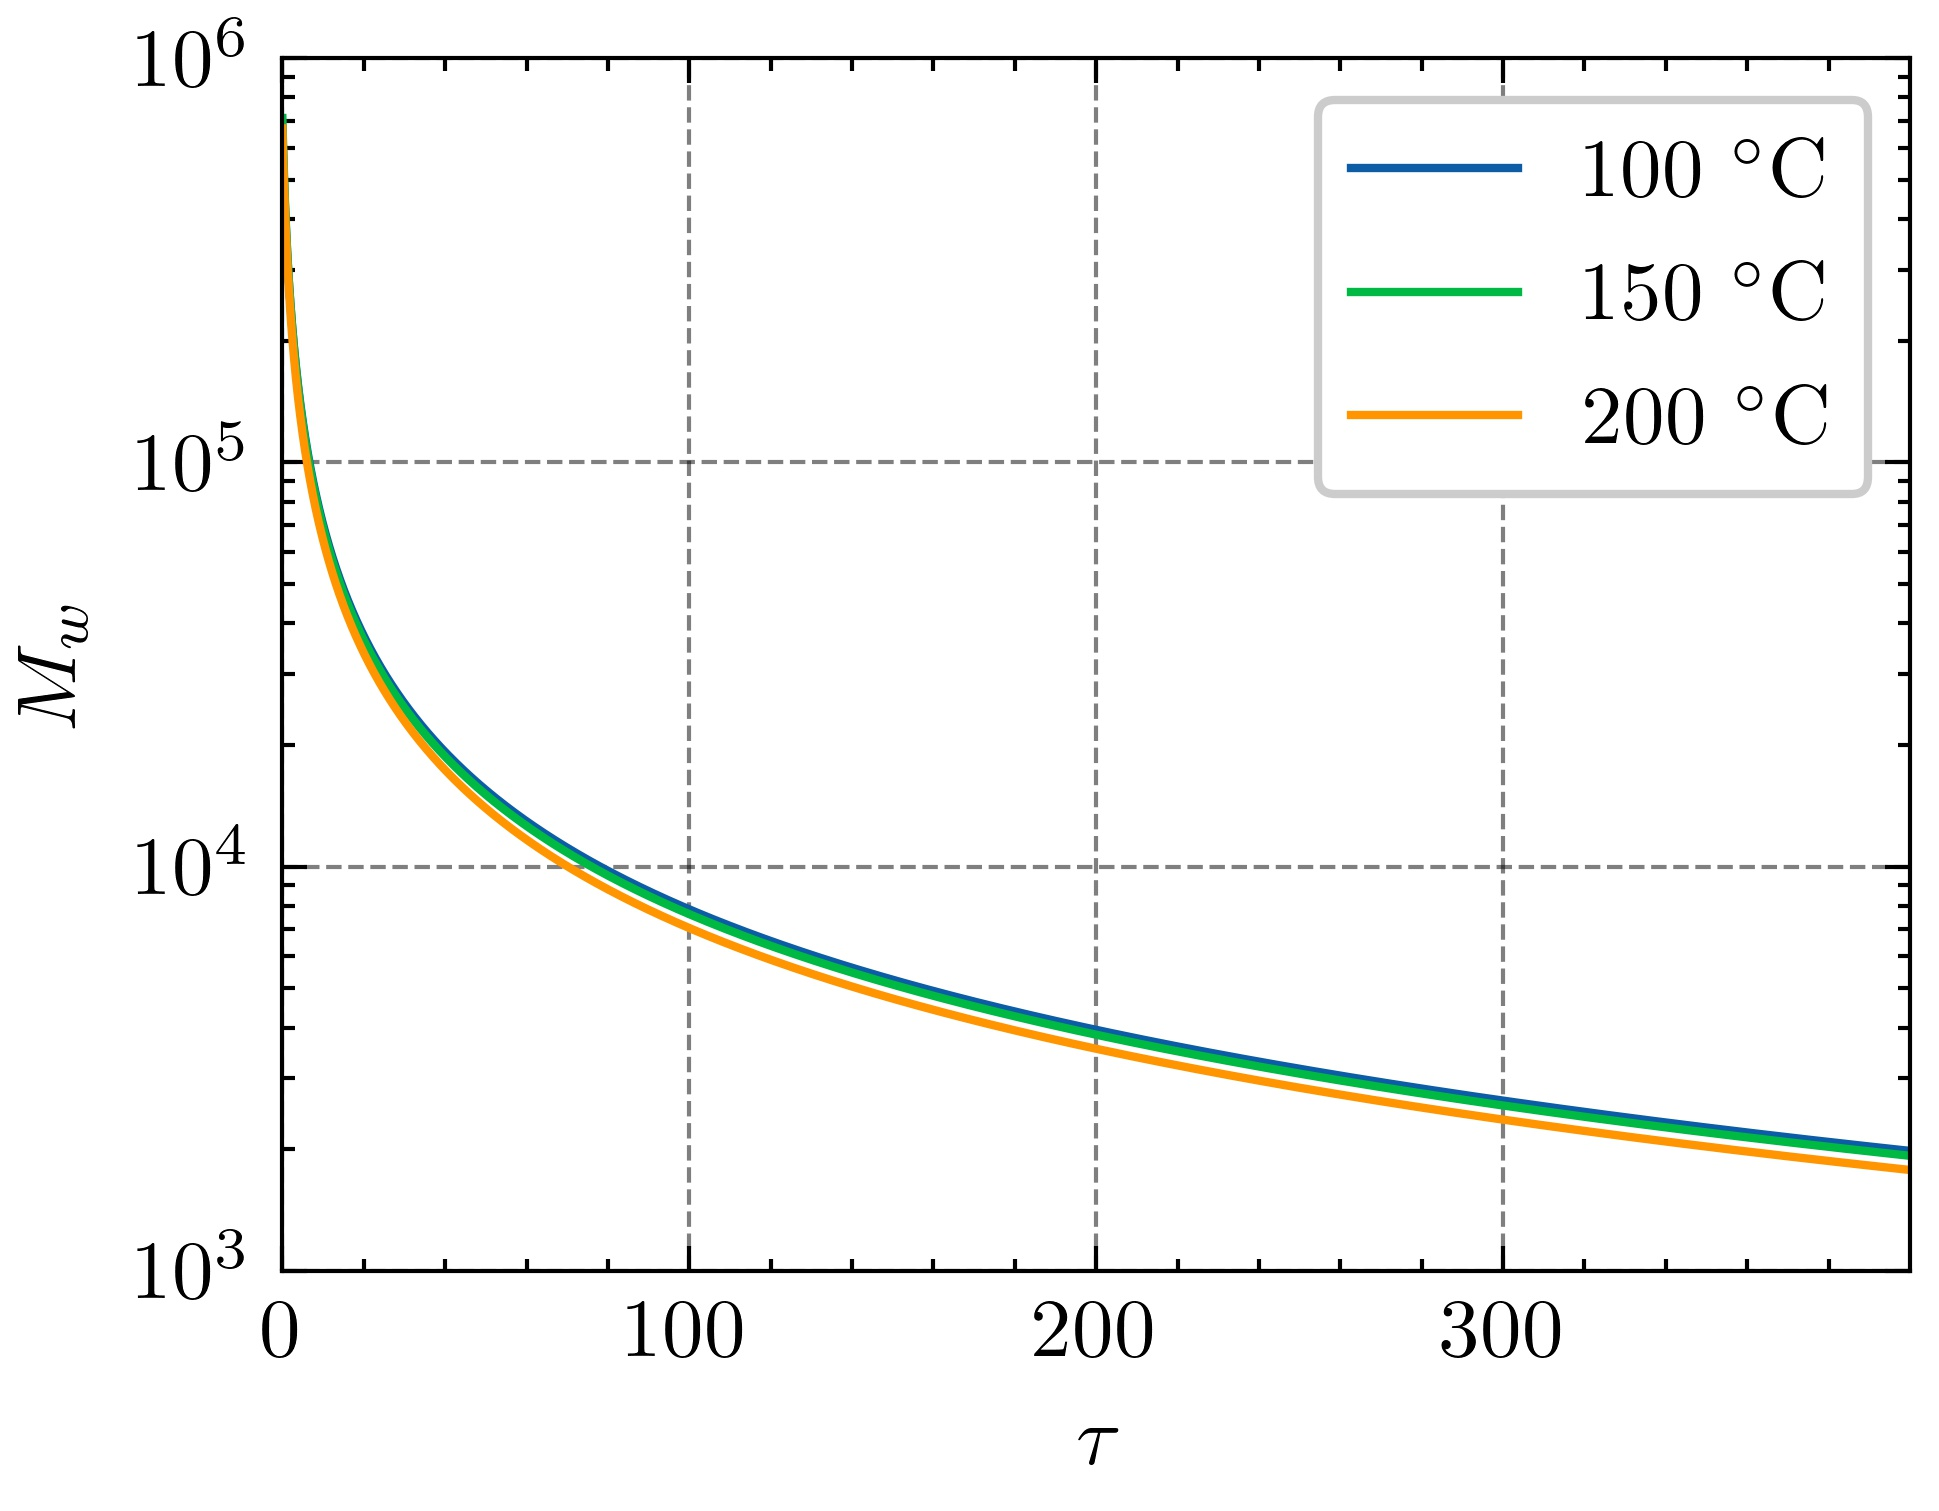
\includegraphics[width=\linewidth]{Mw_tau_100_150_200} \\
		\vspace{-13em} \\ \text{\hspace{-0.1em} b}) \\ \vspace{13em}
	\end{minipage}

	\vspace{-4em}

	\caption{Промоделированные периодические профили с периодом 3 мкм, полученные в слое ПММА с начальной толщиной 500 нм методом СЭЛТР при экспонировании по области с различным распределением плотности тока в пучке. Темпера}
	\label{fig:DEBER_multibeam}
\end{figure}



\begin{figure}[t!]
	\begin{minipage}{0.48\textwidth}
		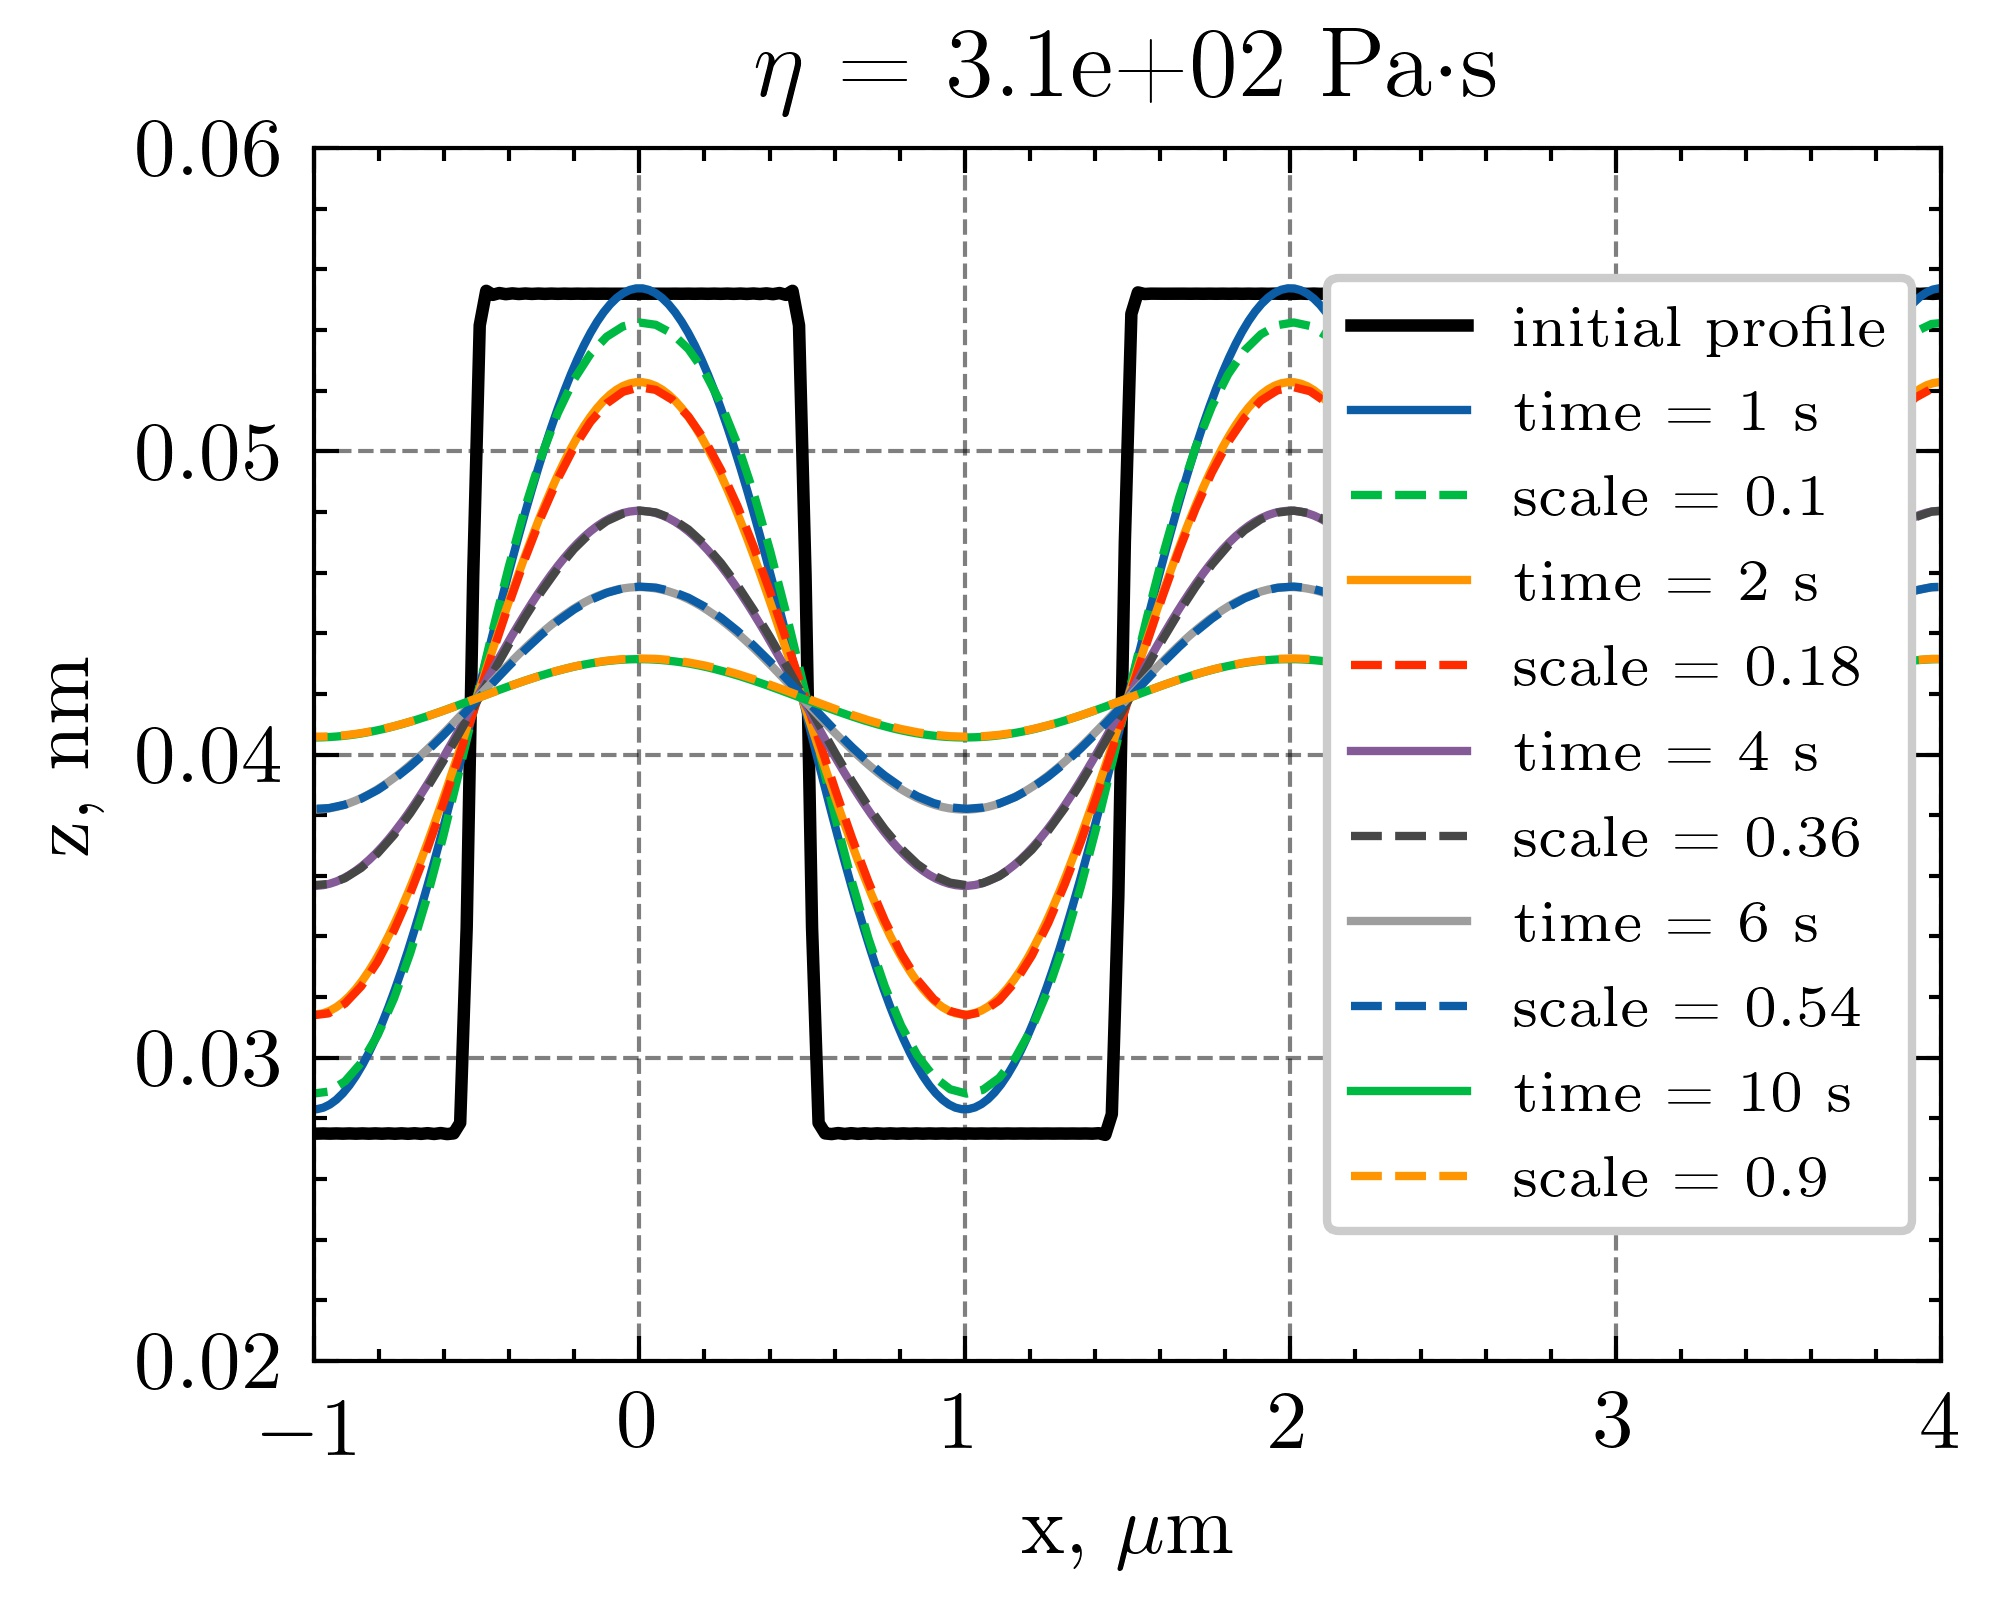
\includegraphics[width=\linewidth]{grating_eta_310} \\
		\vspace{-13em} \\ \text{\hspace{0em} a}) \\ \vspace{13em}
	\end{minipage}
	\begin{minipage}{0.48\textwidth}
		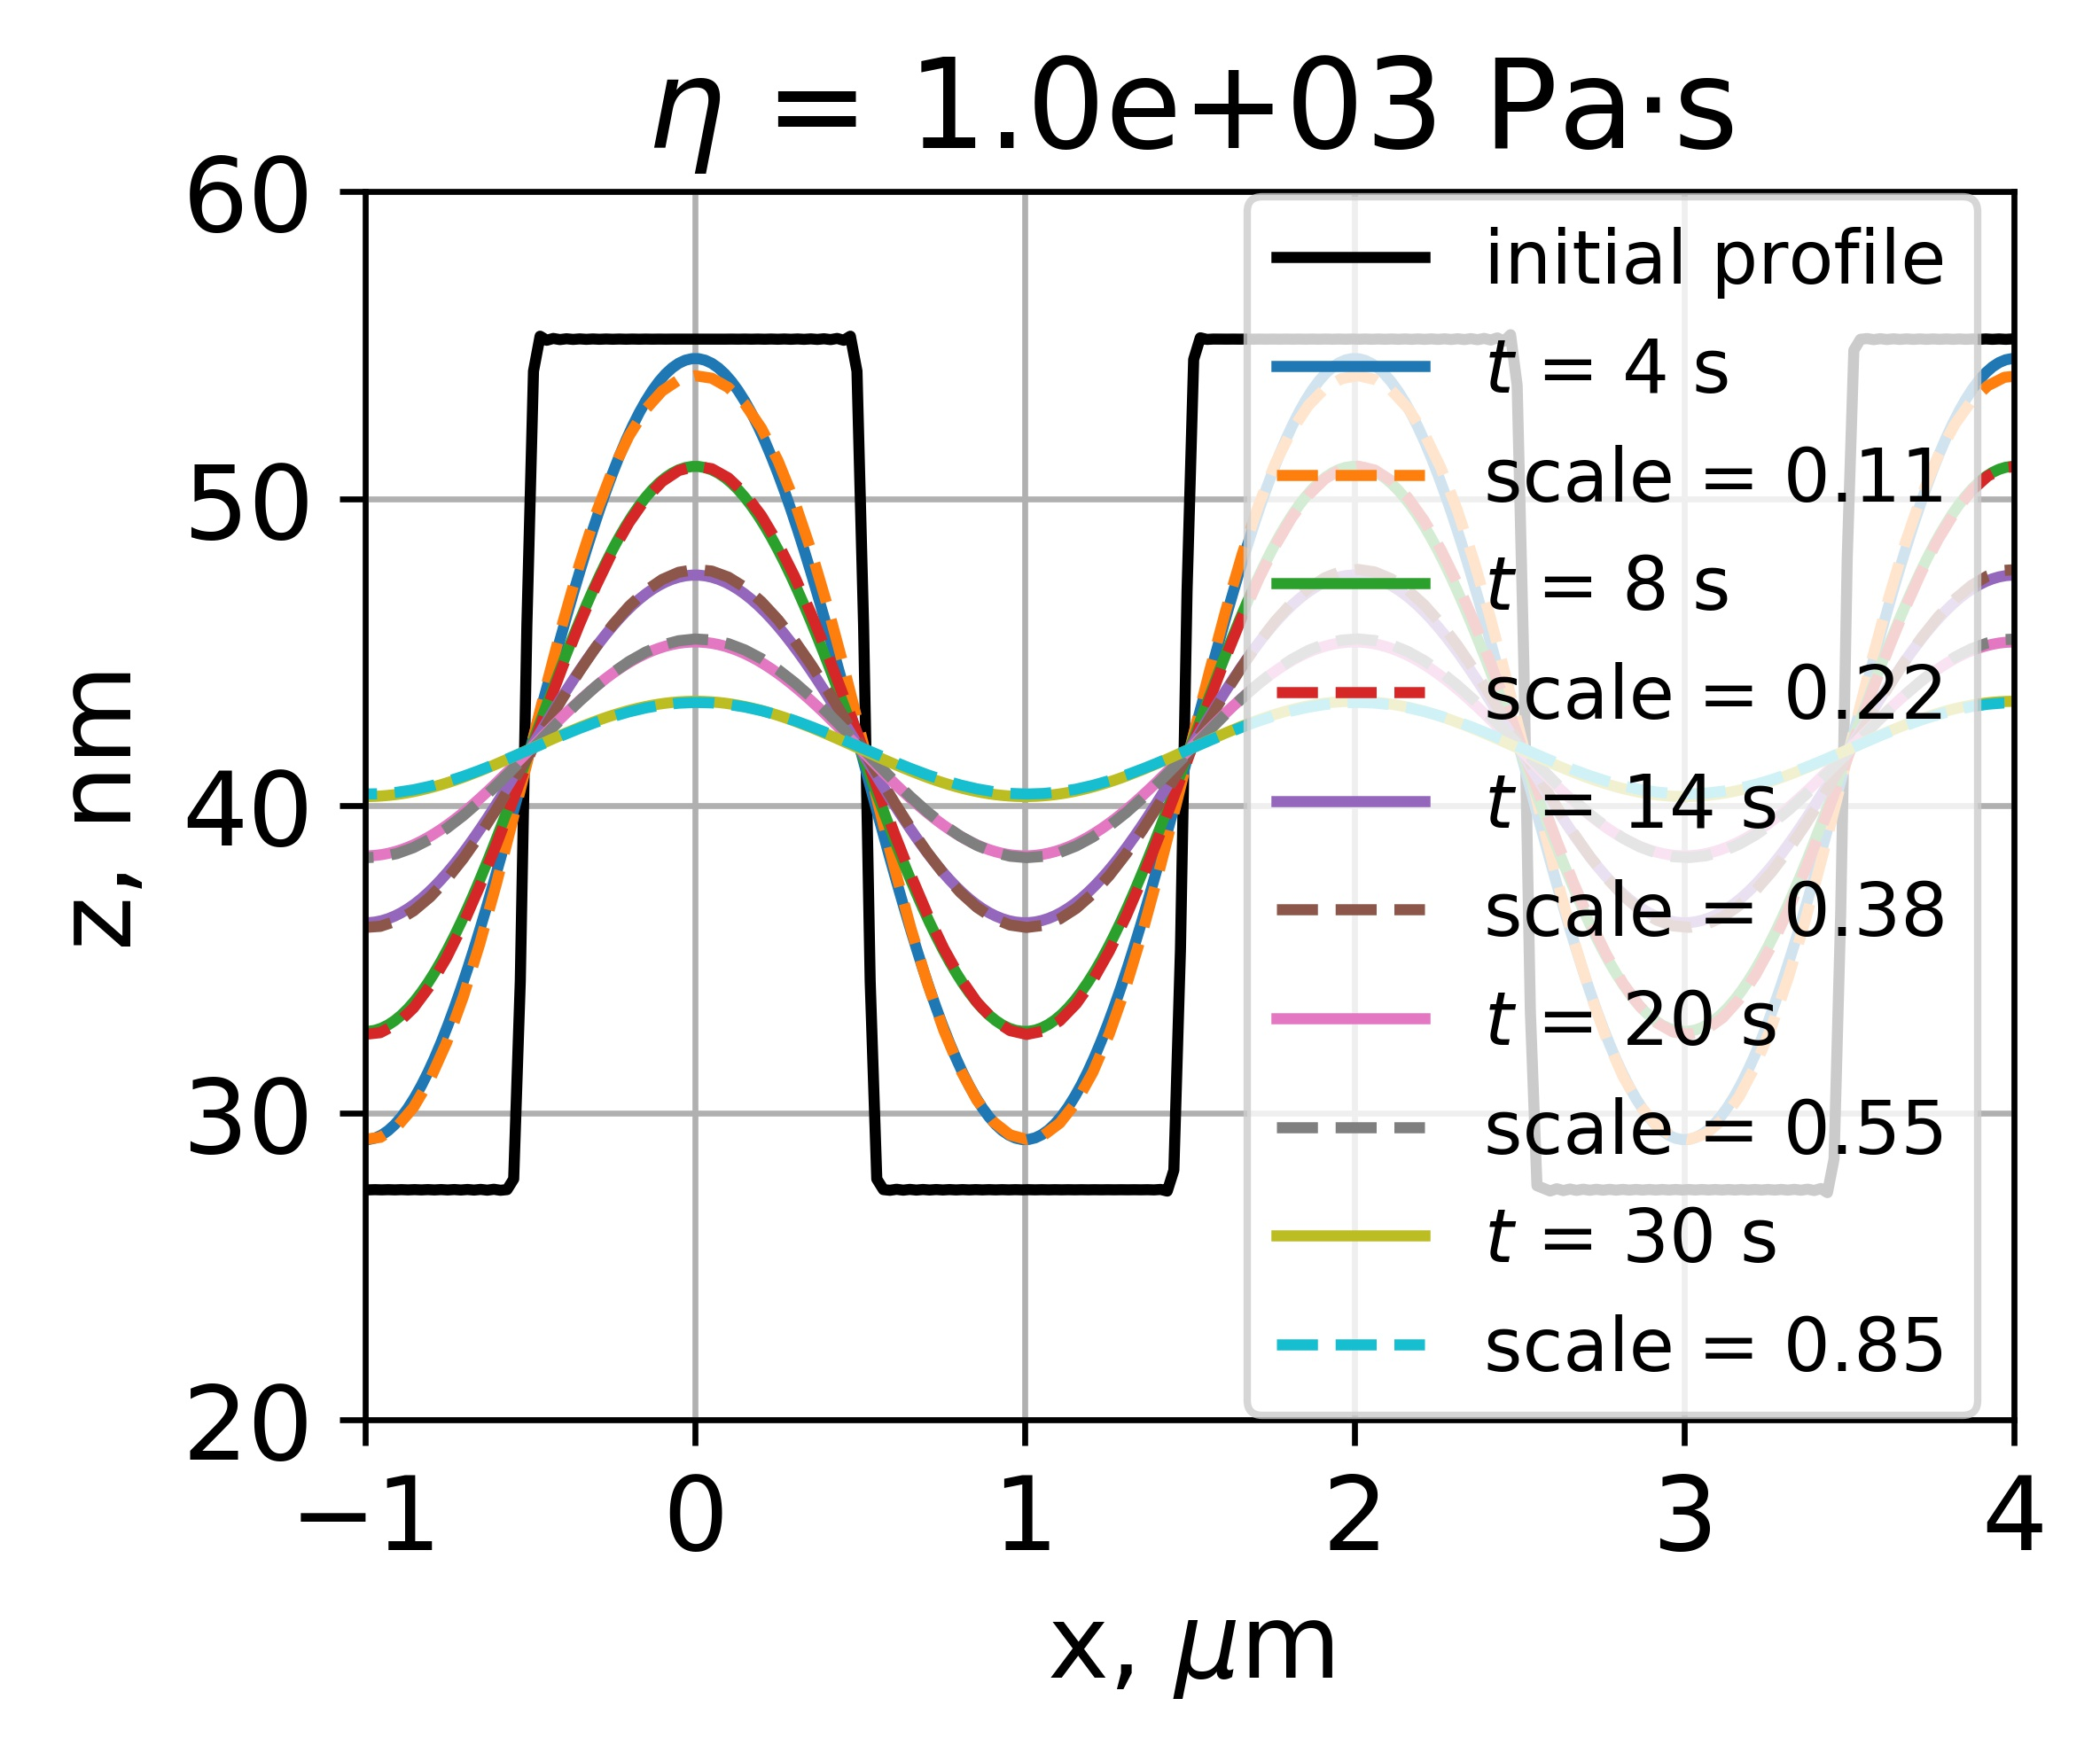
\includegraphics[width=\linewidth]{grating_eta_1000} \\
		\vspace{-13em} \\ \text{\hspace{-0.1em} b}) \\ \vspace{13em}
	\end{minipage}
	
	\vspace{-3em}
	
	\begin{minipage}{0.48\textwidth}
		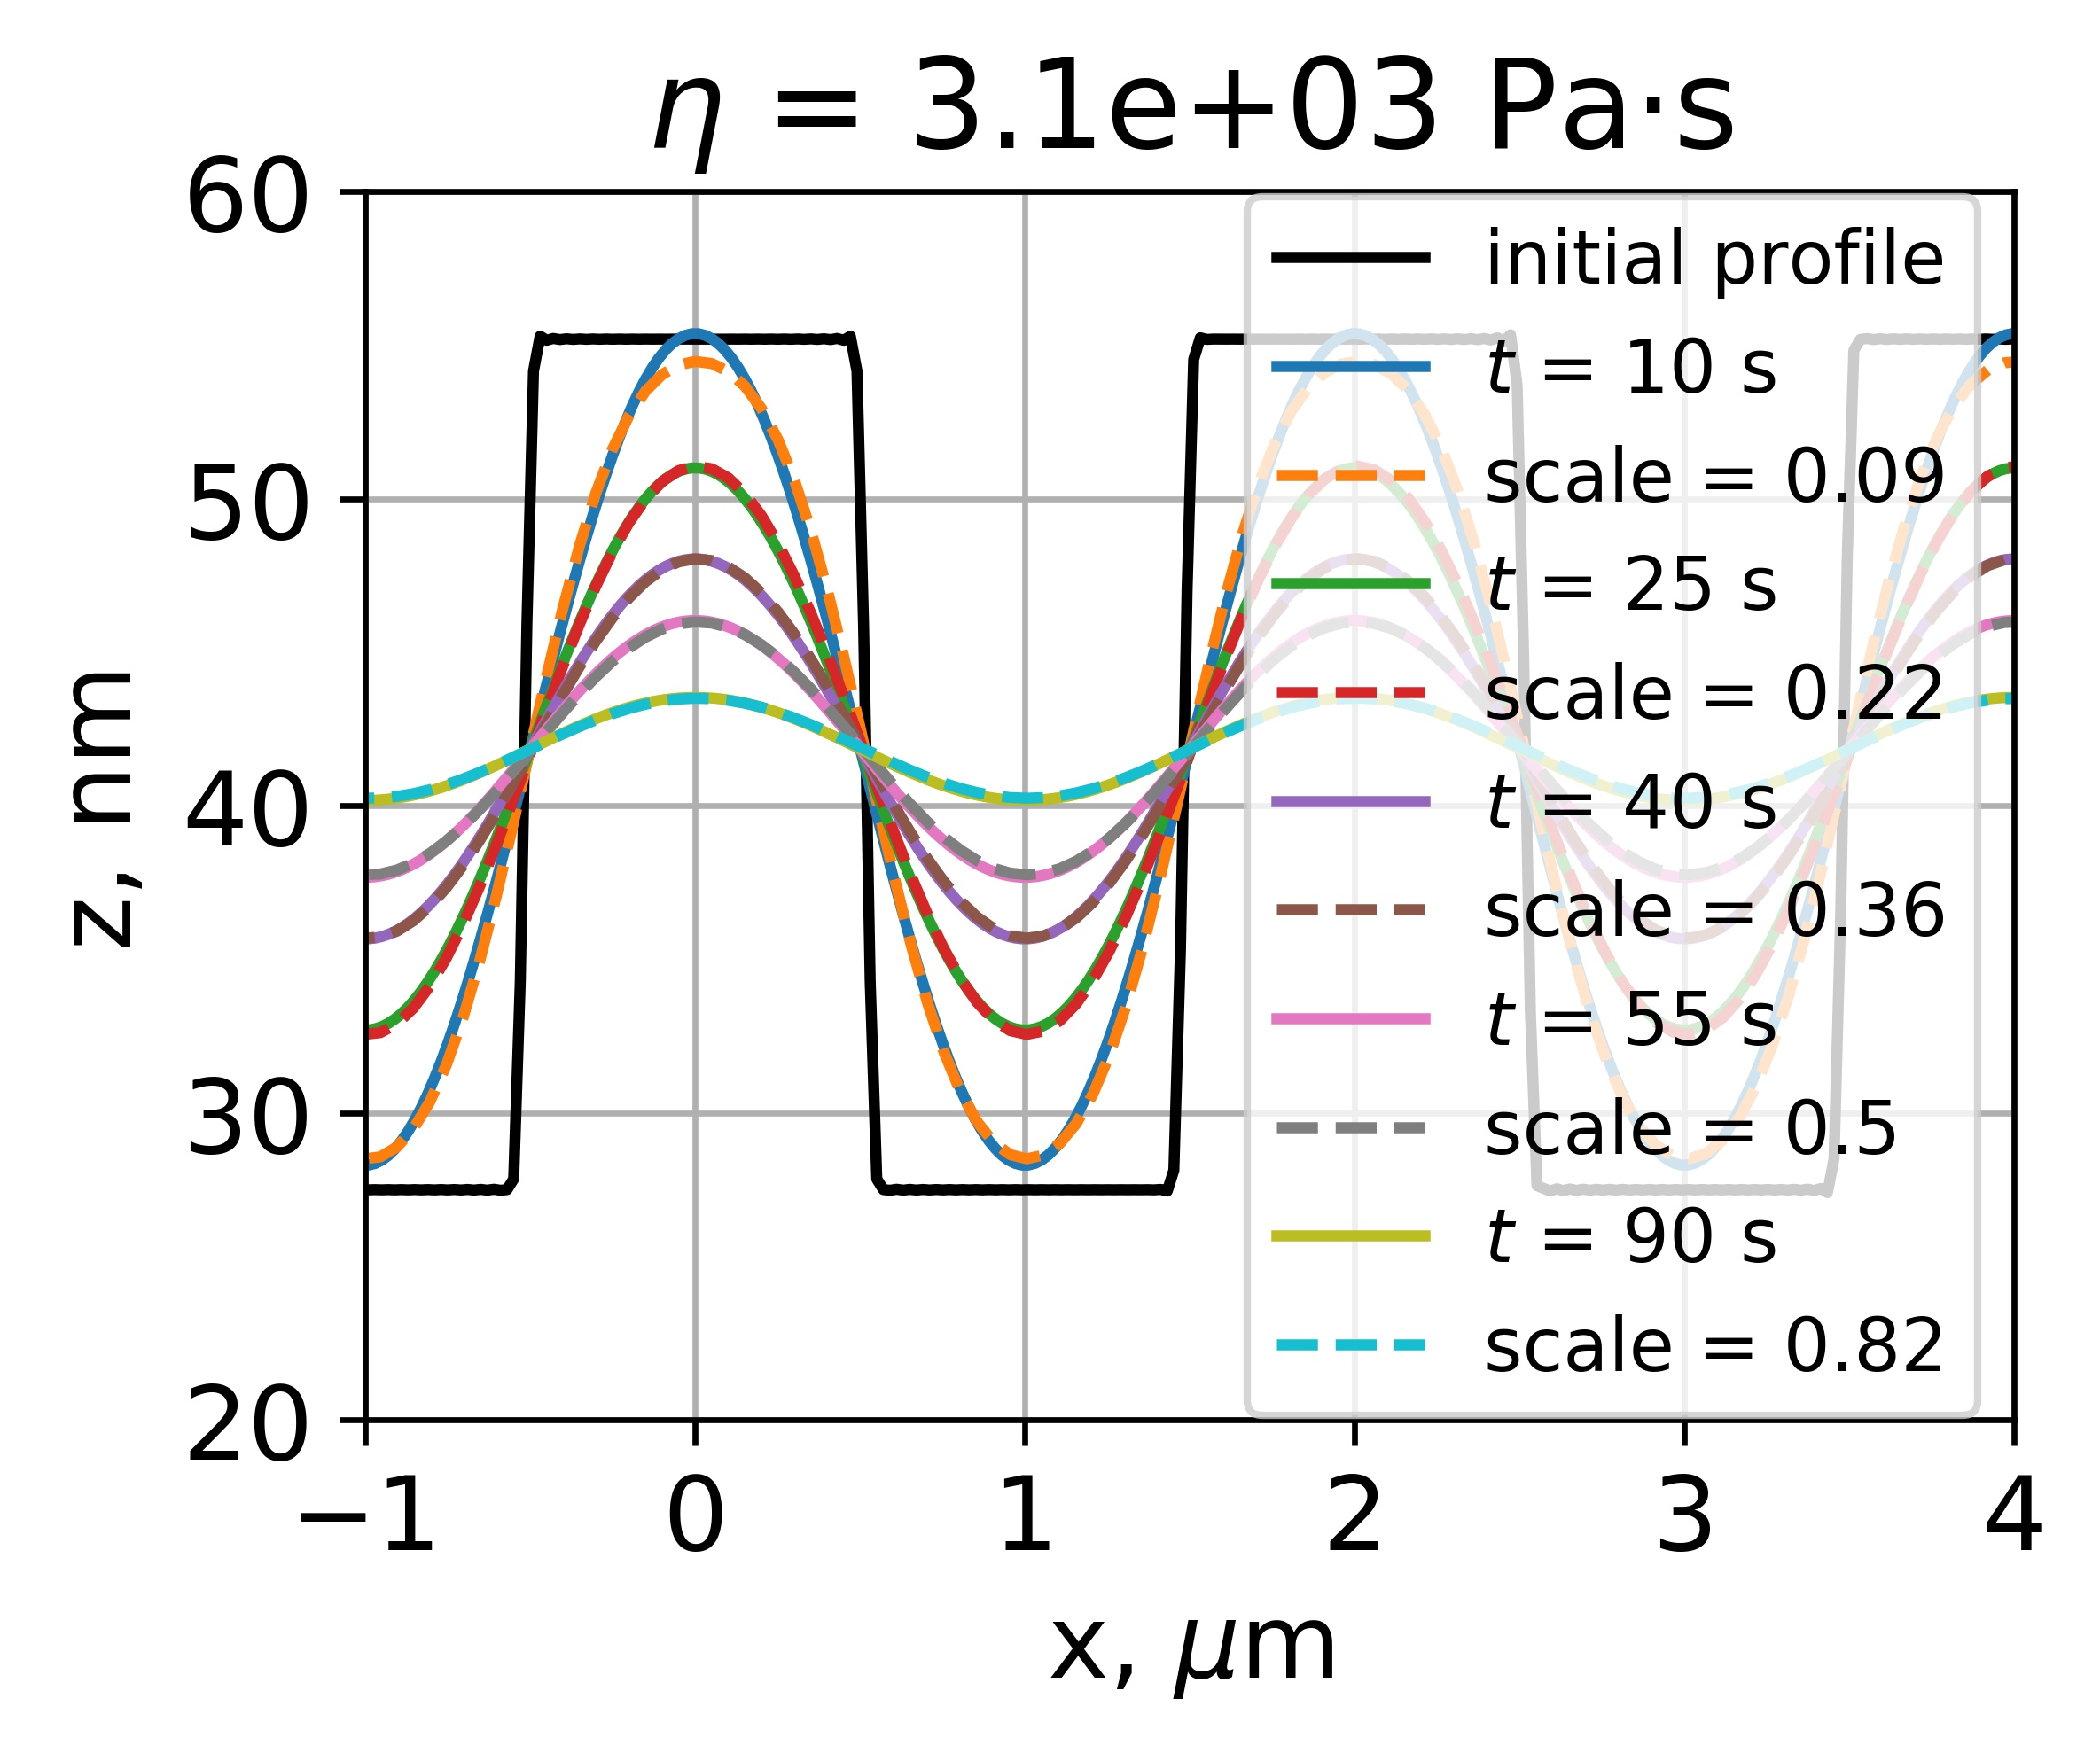
\includegraphics[width=\linewidth]{grating_eta_3100} \\
		\vspace{-13em} \\ \text{\hspace{0em} c}) \\ \vspace{13em}
	\end{minipage}
	\begin{minipage}{0.48\textwidth}
		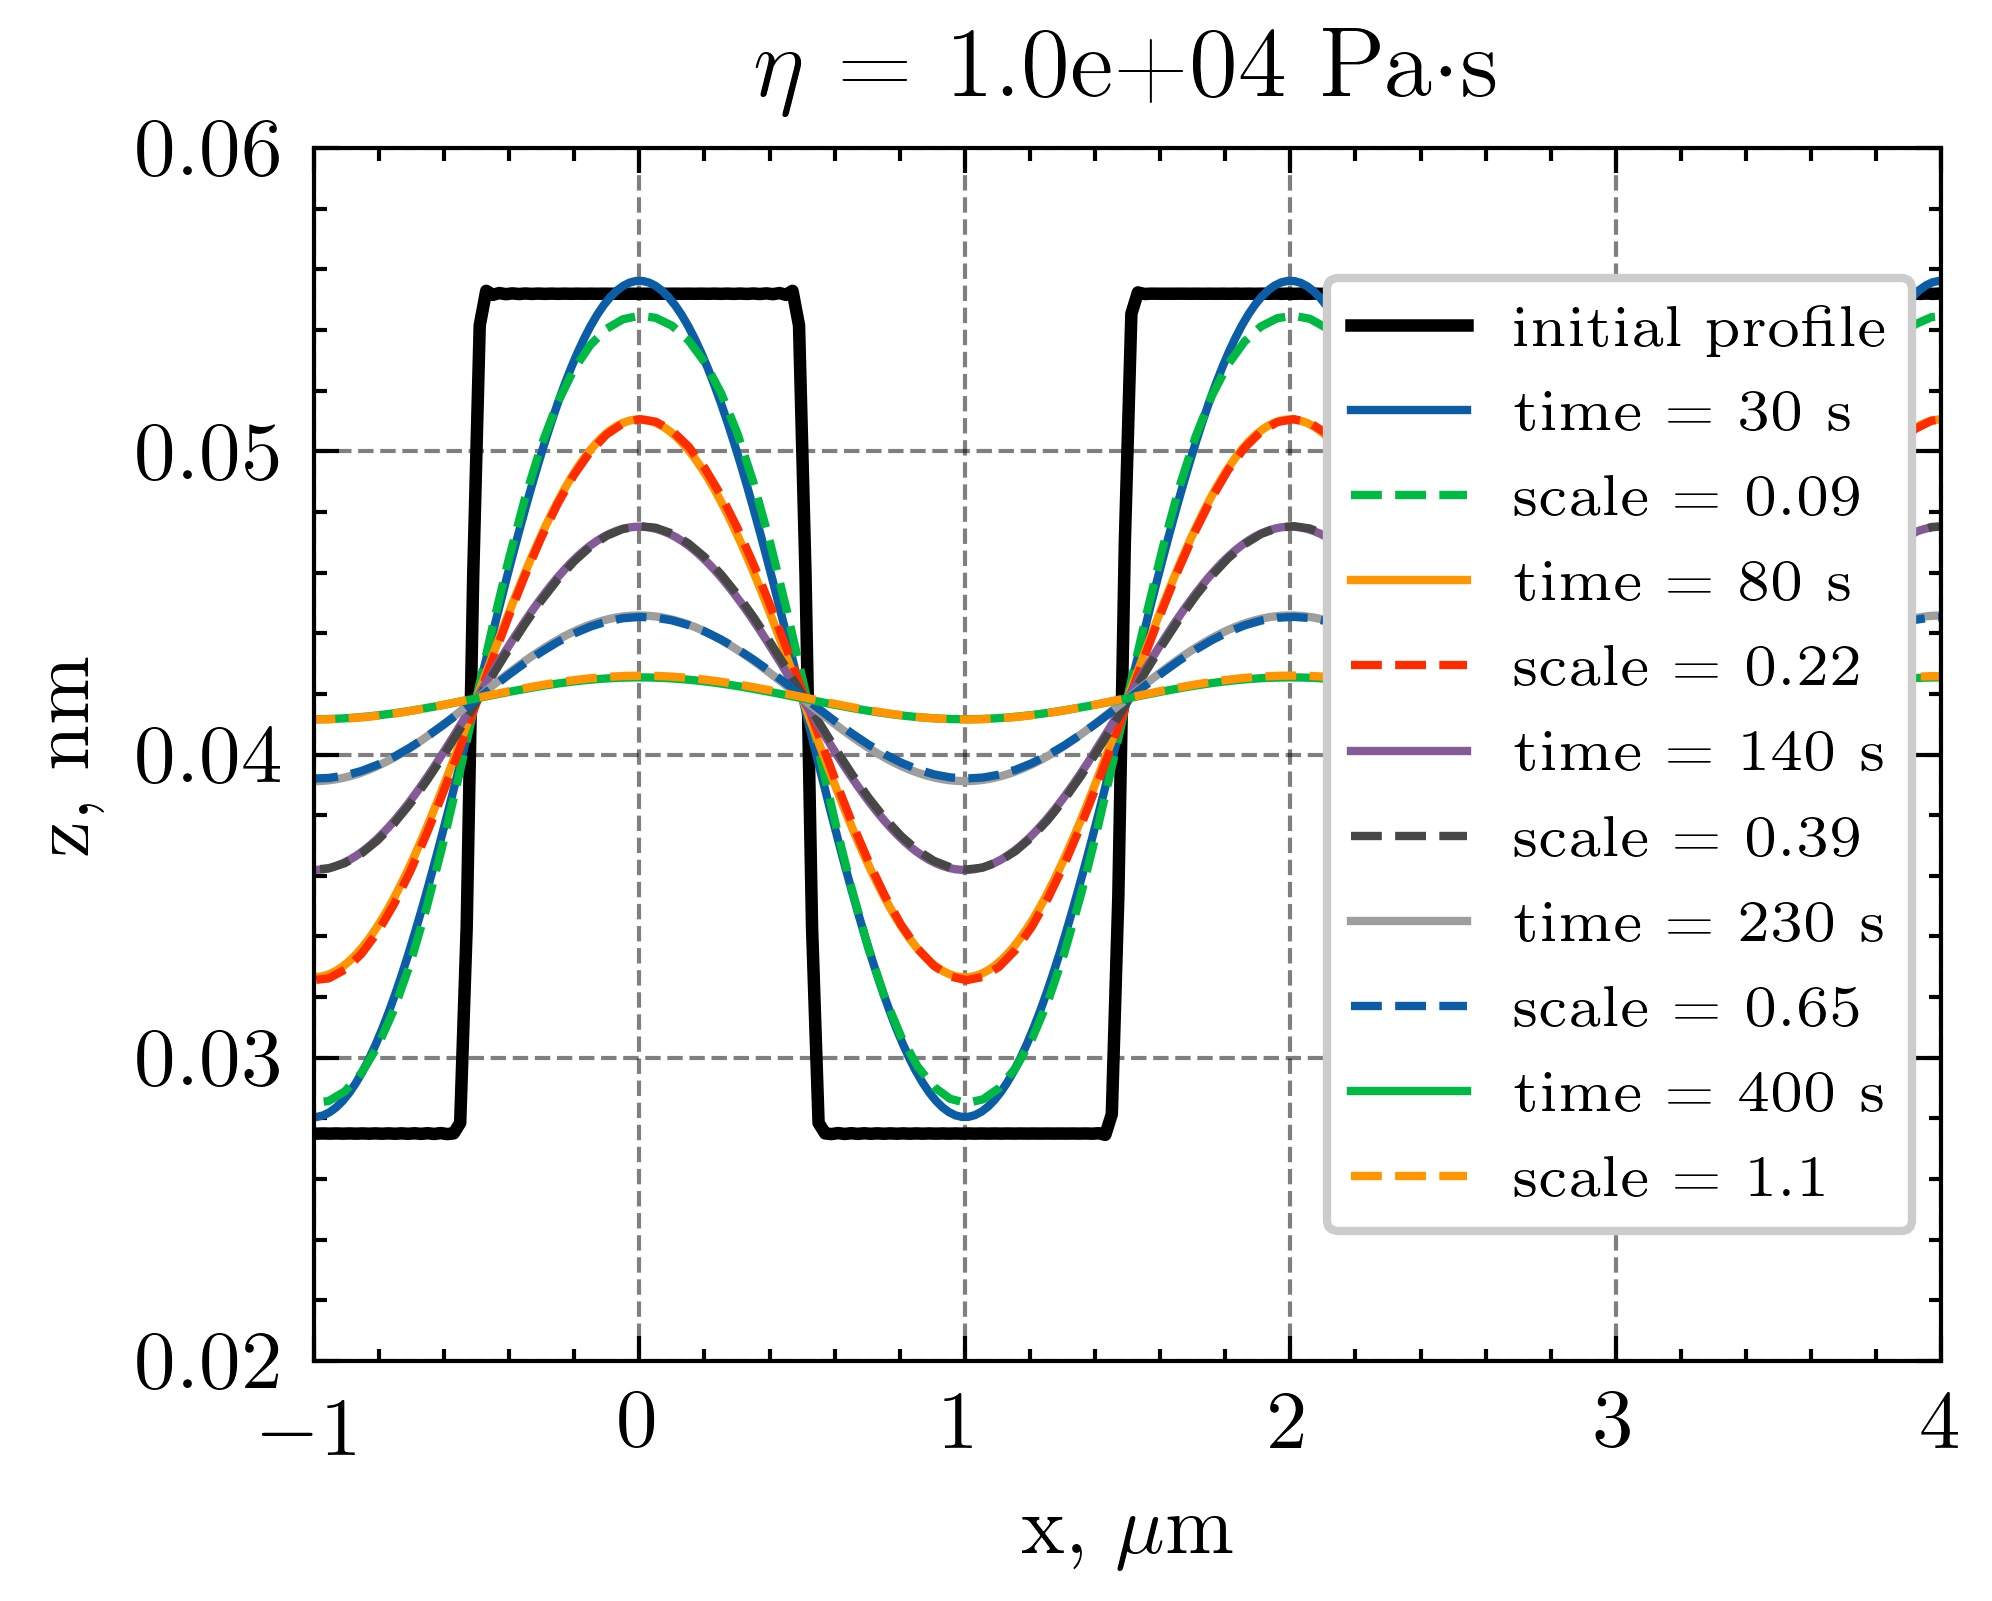
\includegraphics[width=\linewidth]{grating_eta_10000} \\
		\vspace{-13em} \\ \text{\hspace{-0.1em} d}) \\ \vspace{13em}
	\end{minipage}

	\vspace{-3em}
	
	\begin{minipage}{0.48\textwidth}
		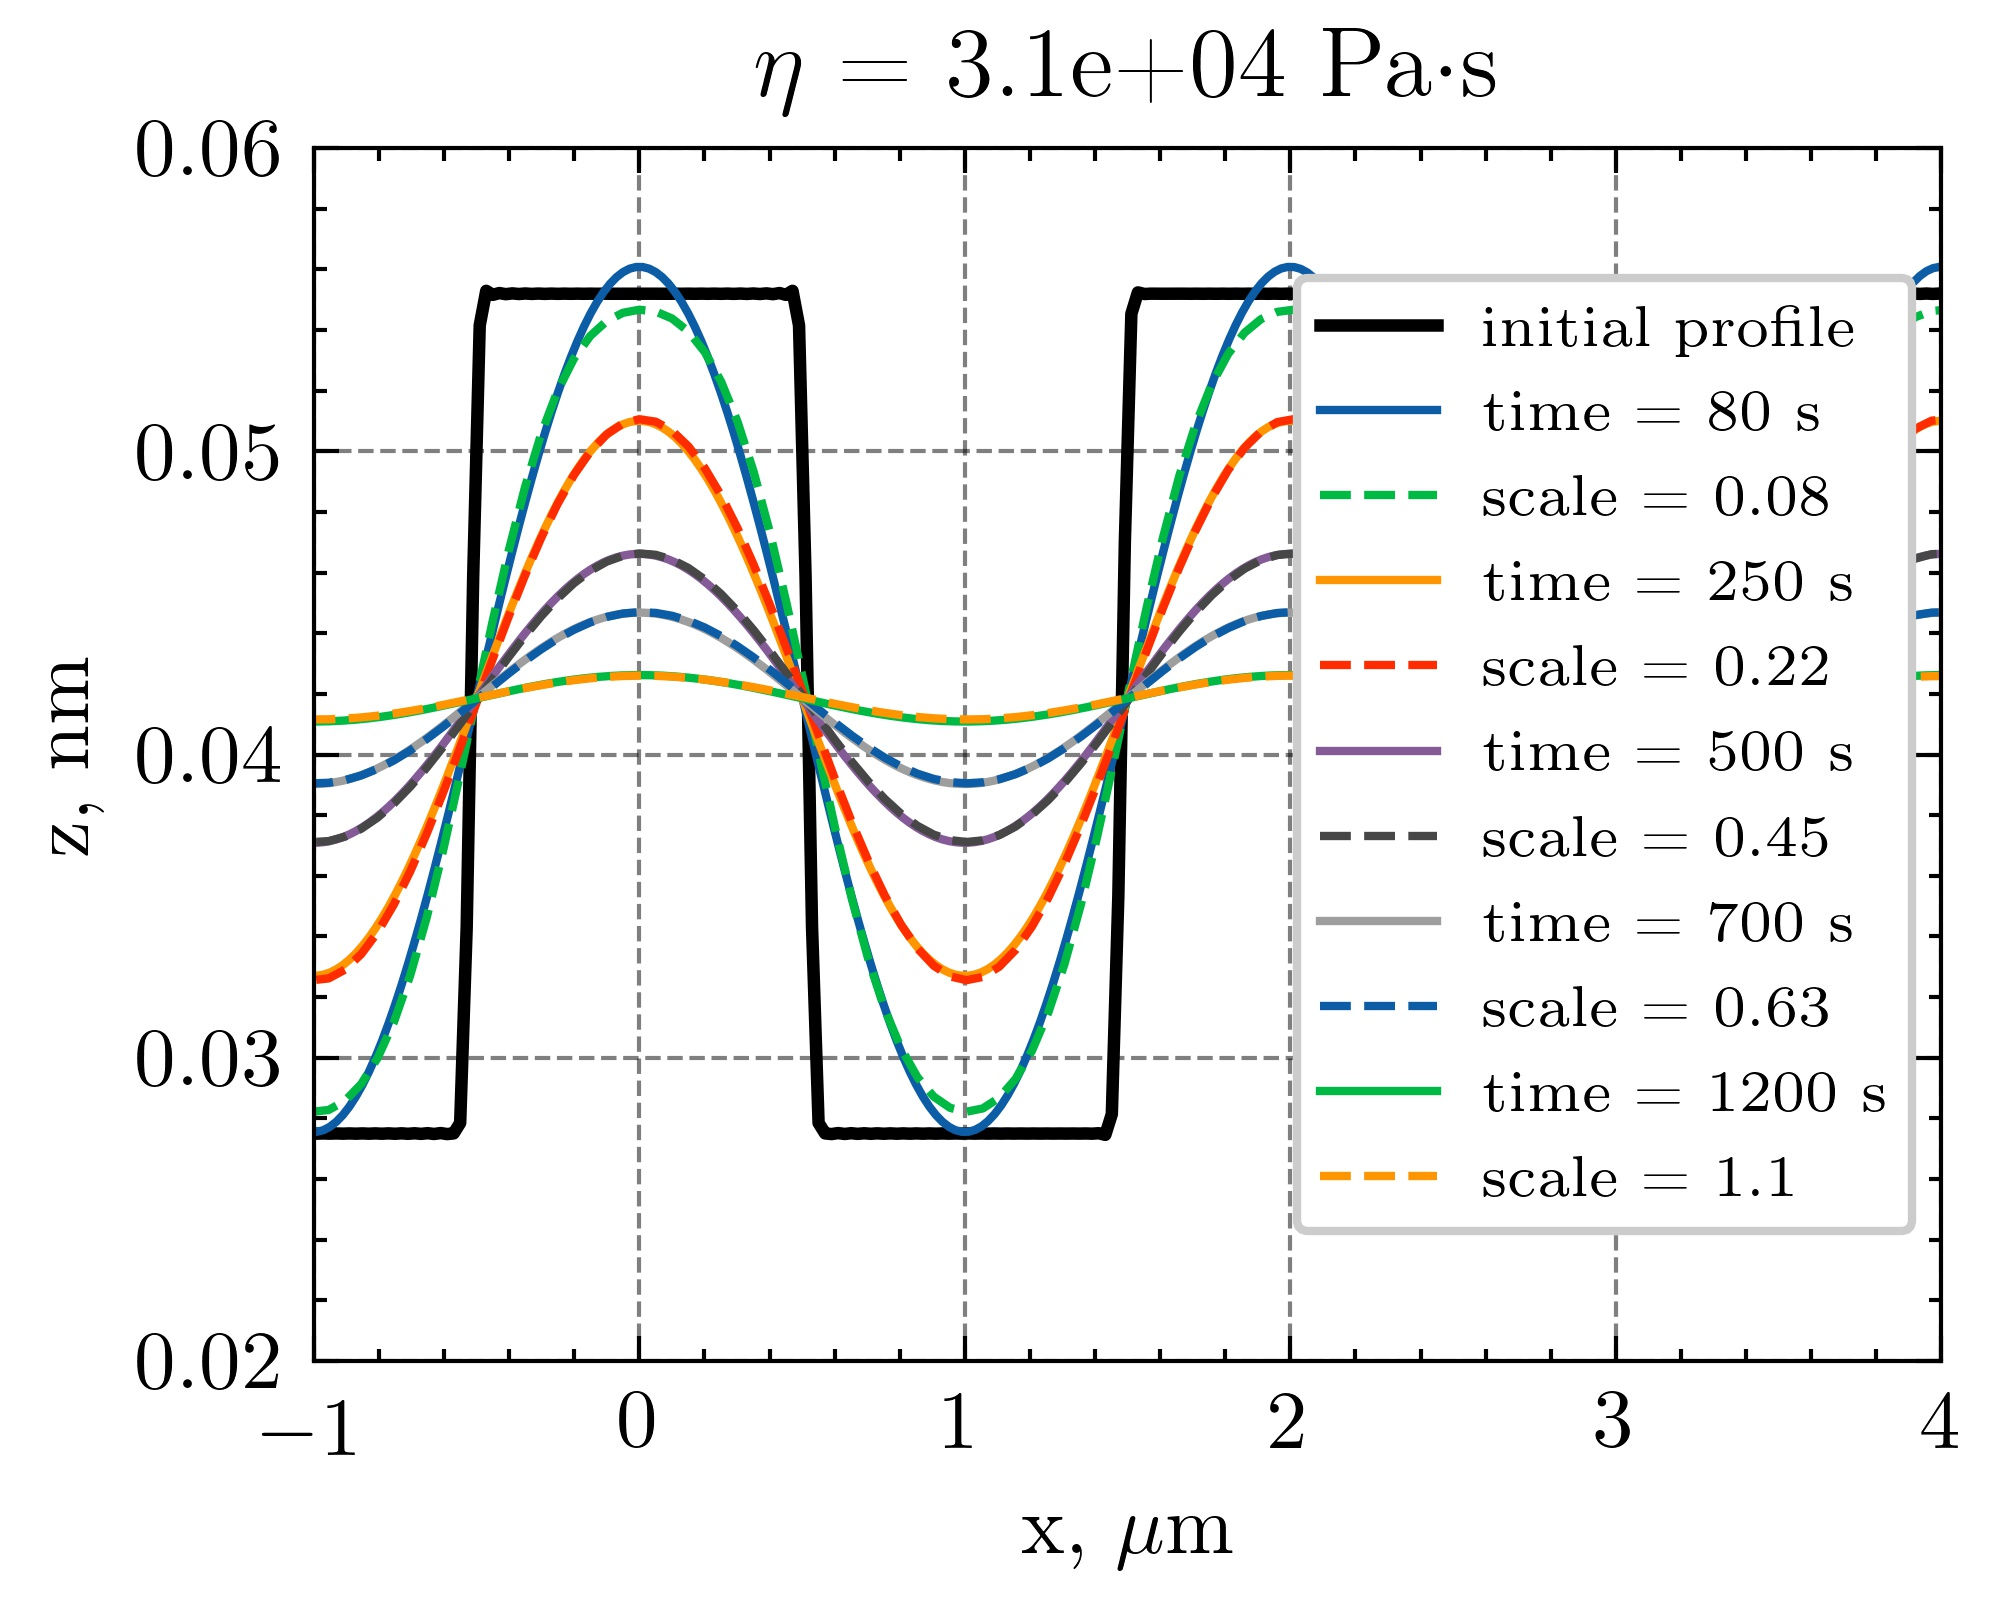
\includegraphics[width=\linewidth]{grating_eta_31000} \\
		\vspace{-13em} \\ \text{\hspace{0em} c}) \\ \vspace{13em}
	\end{minipage}
	\begin{minipage}{0.48\textwidth}
		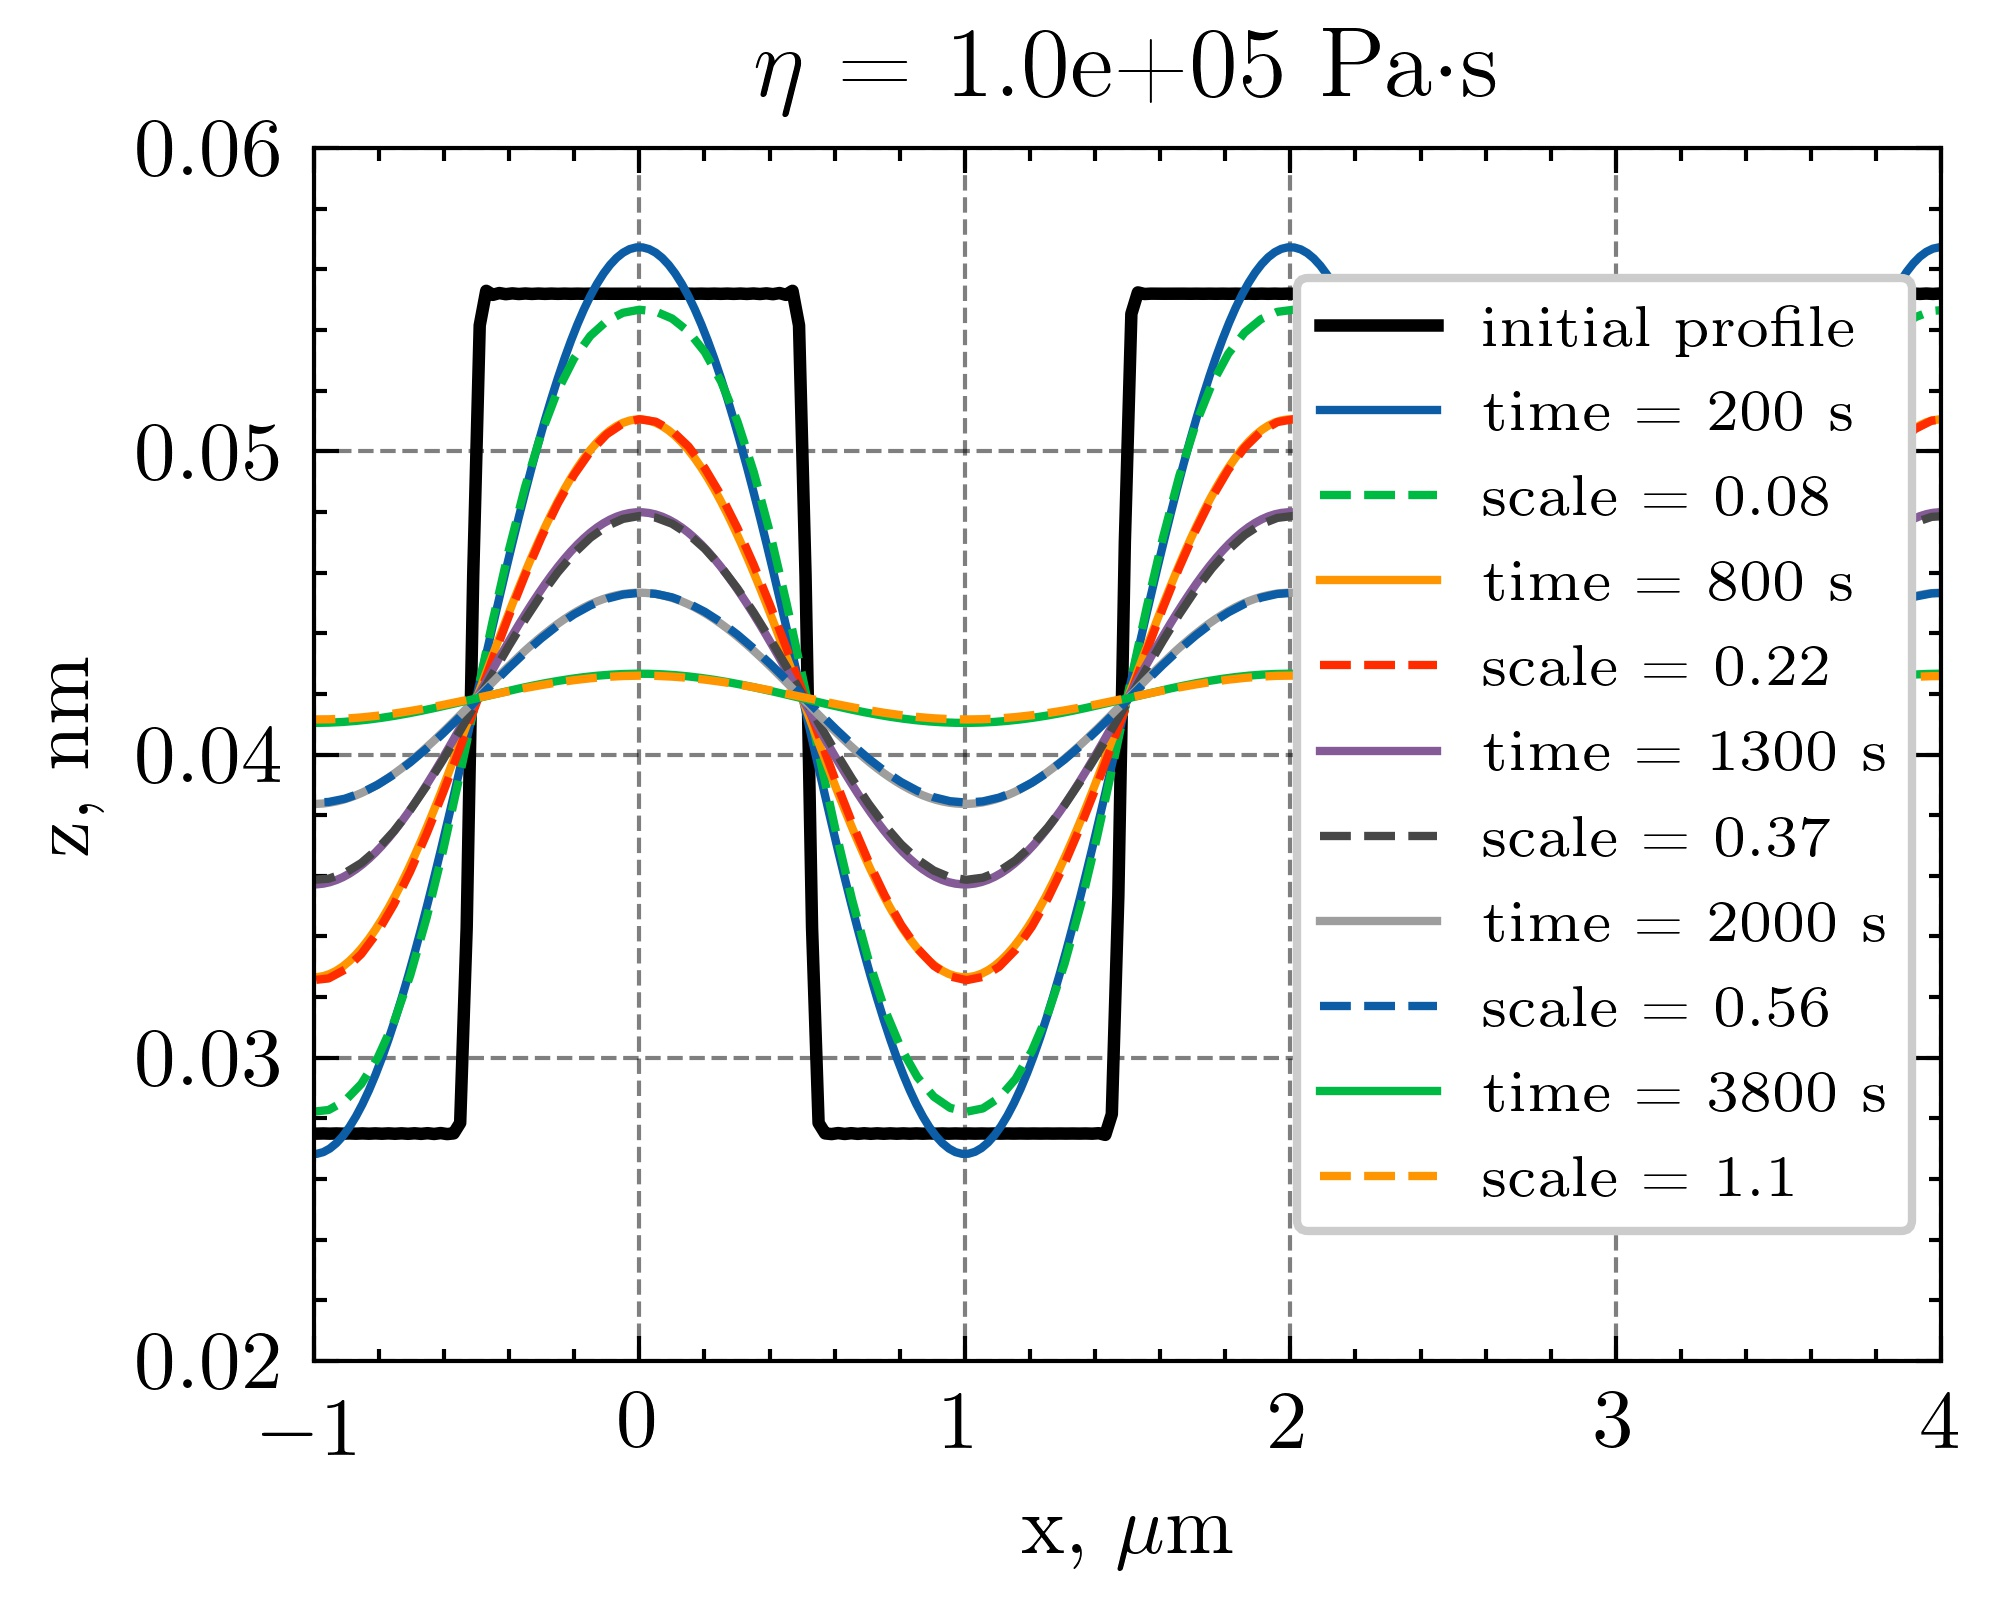
\includegraphics[width=\linewidth]{grating_eta_100000} \\
		\vspace{-13em} \\ \text{\hspace{-0.1em} d}) \\ \vspace{13em}
	\end{minipage}

	\vspace{-4em}
	
	\caption{Промоделированные периодические профили с периодом 3 мкм, полученные в слое ПММА с начальной толщиной 500 нм методом СЭЛТР при экспонировании по области с различным распределением плотности тока в пучке. Темпера}
	\label{fig:DEBER_multibeam}
\end{figure}


\begin{figure}[t!]
	\begin{minipage}{0.48\textwidth}
		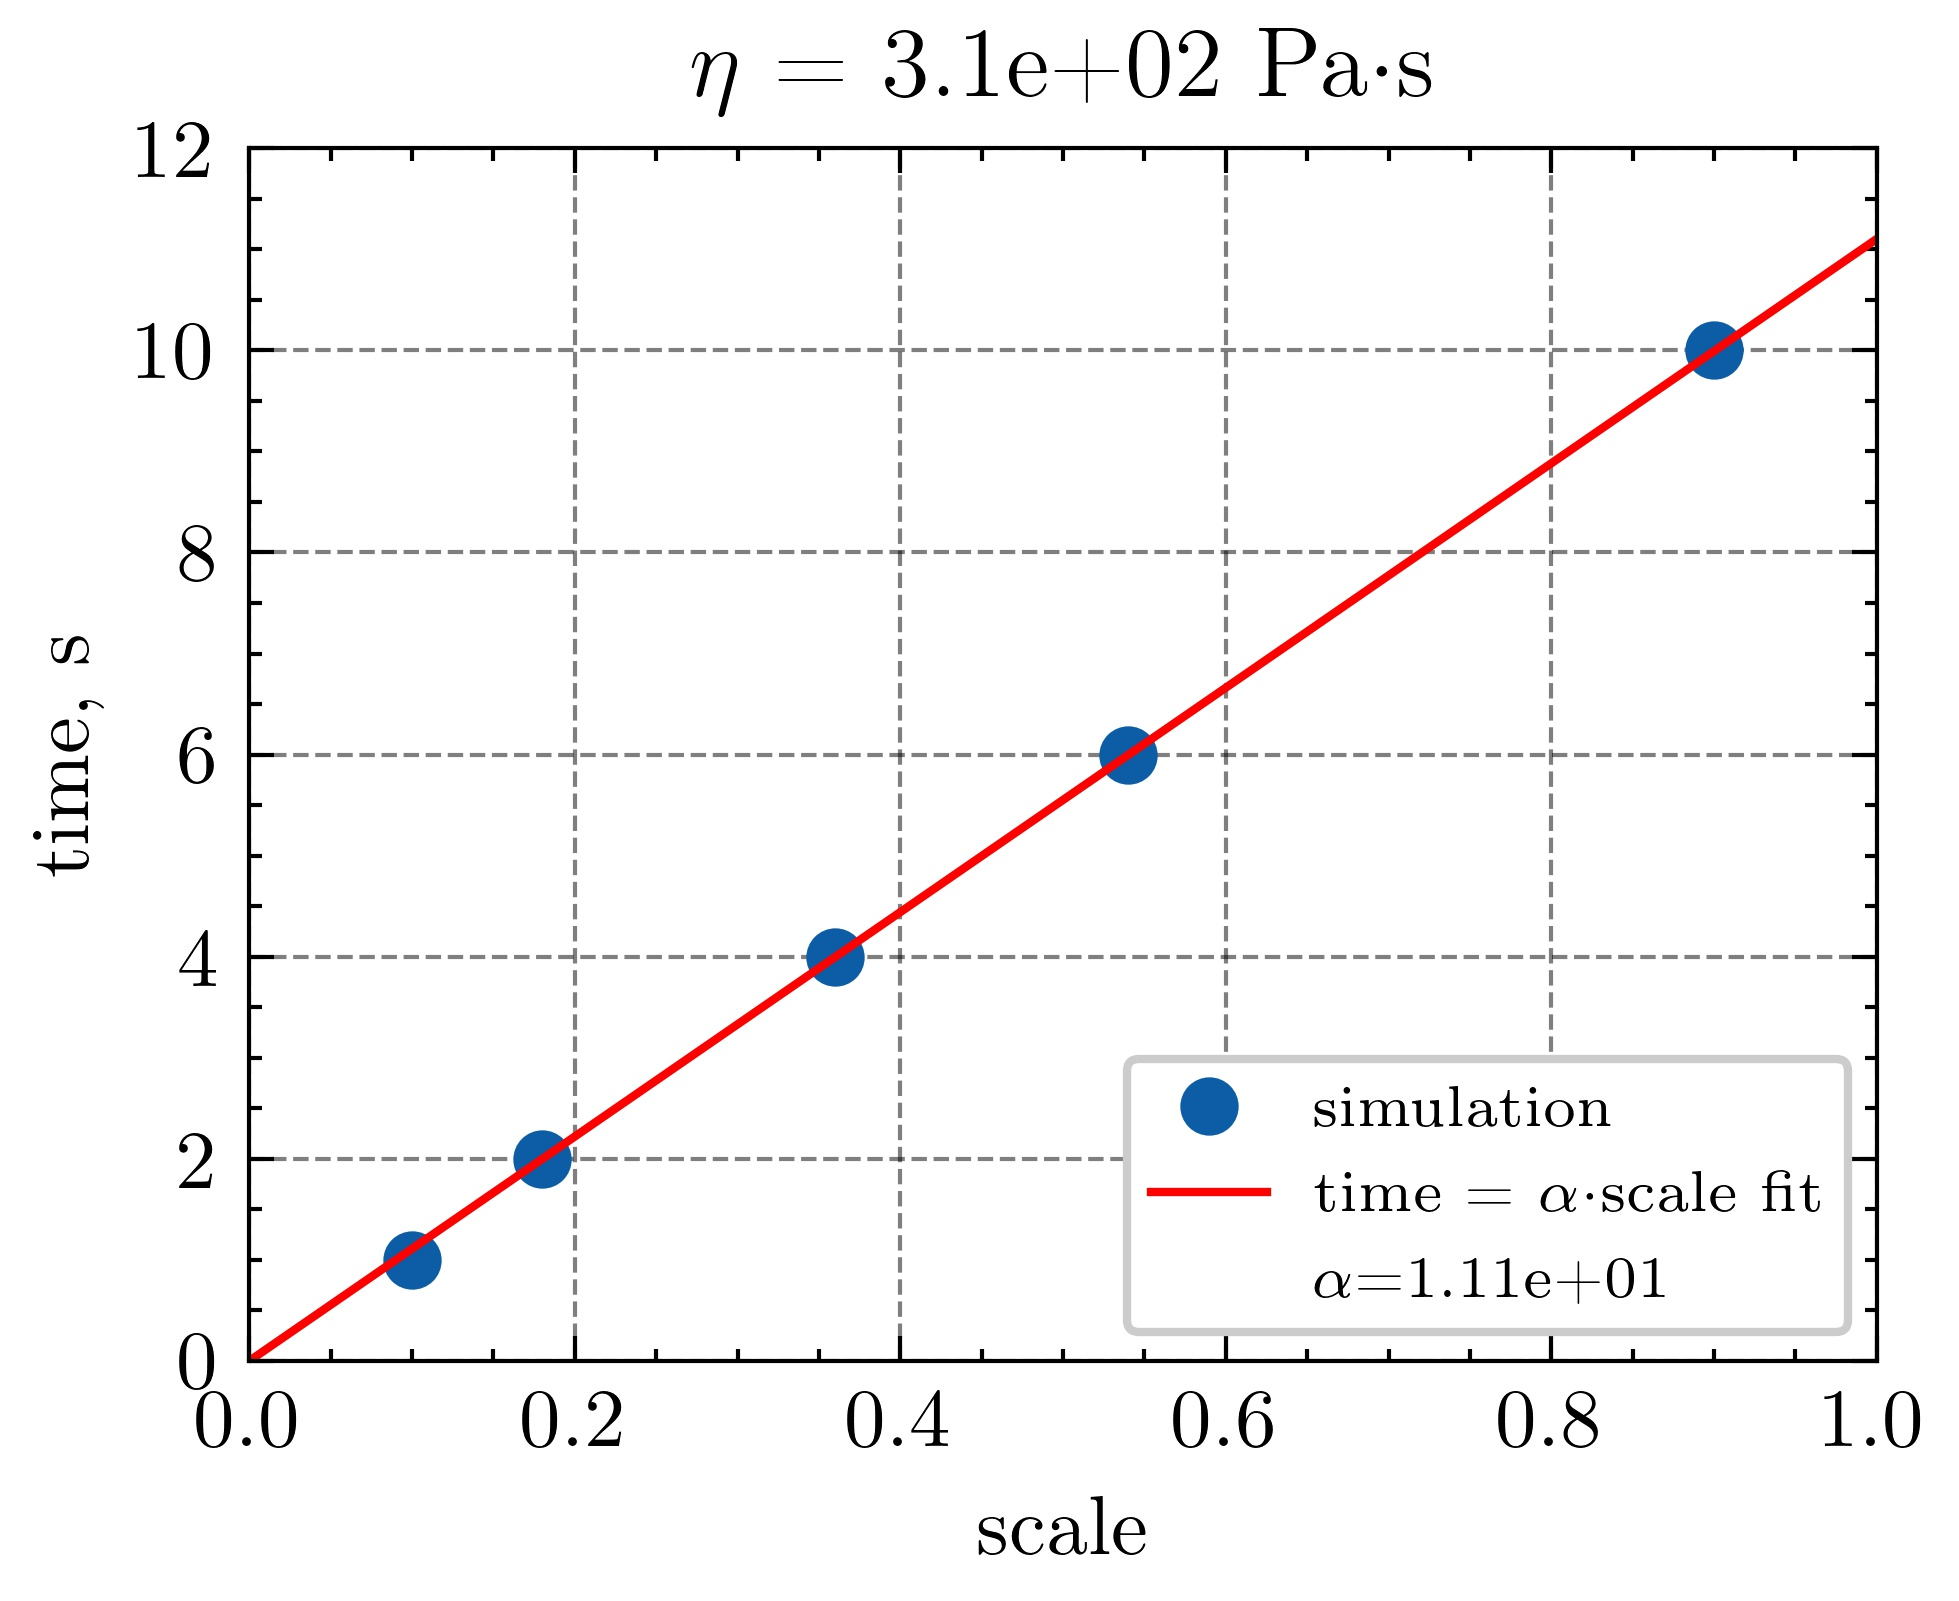
\includegraphics[width=\linewidth]{alpha_310} \\
		\vspace{-13em} \\ \text{\hspace{0em} a}) \\ \vspace{13em}
	\end{minipage}
	\begin{minipage}{0.48\textwidth}
		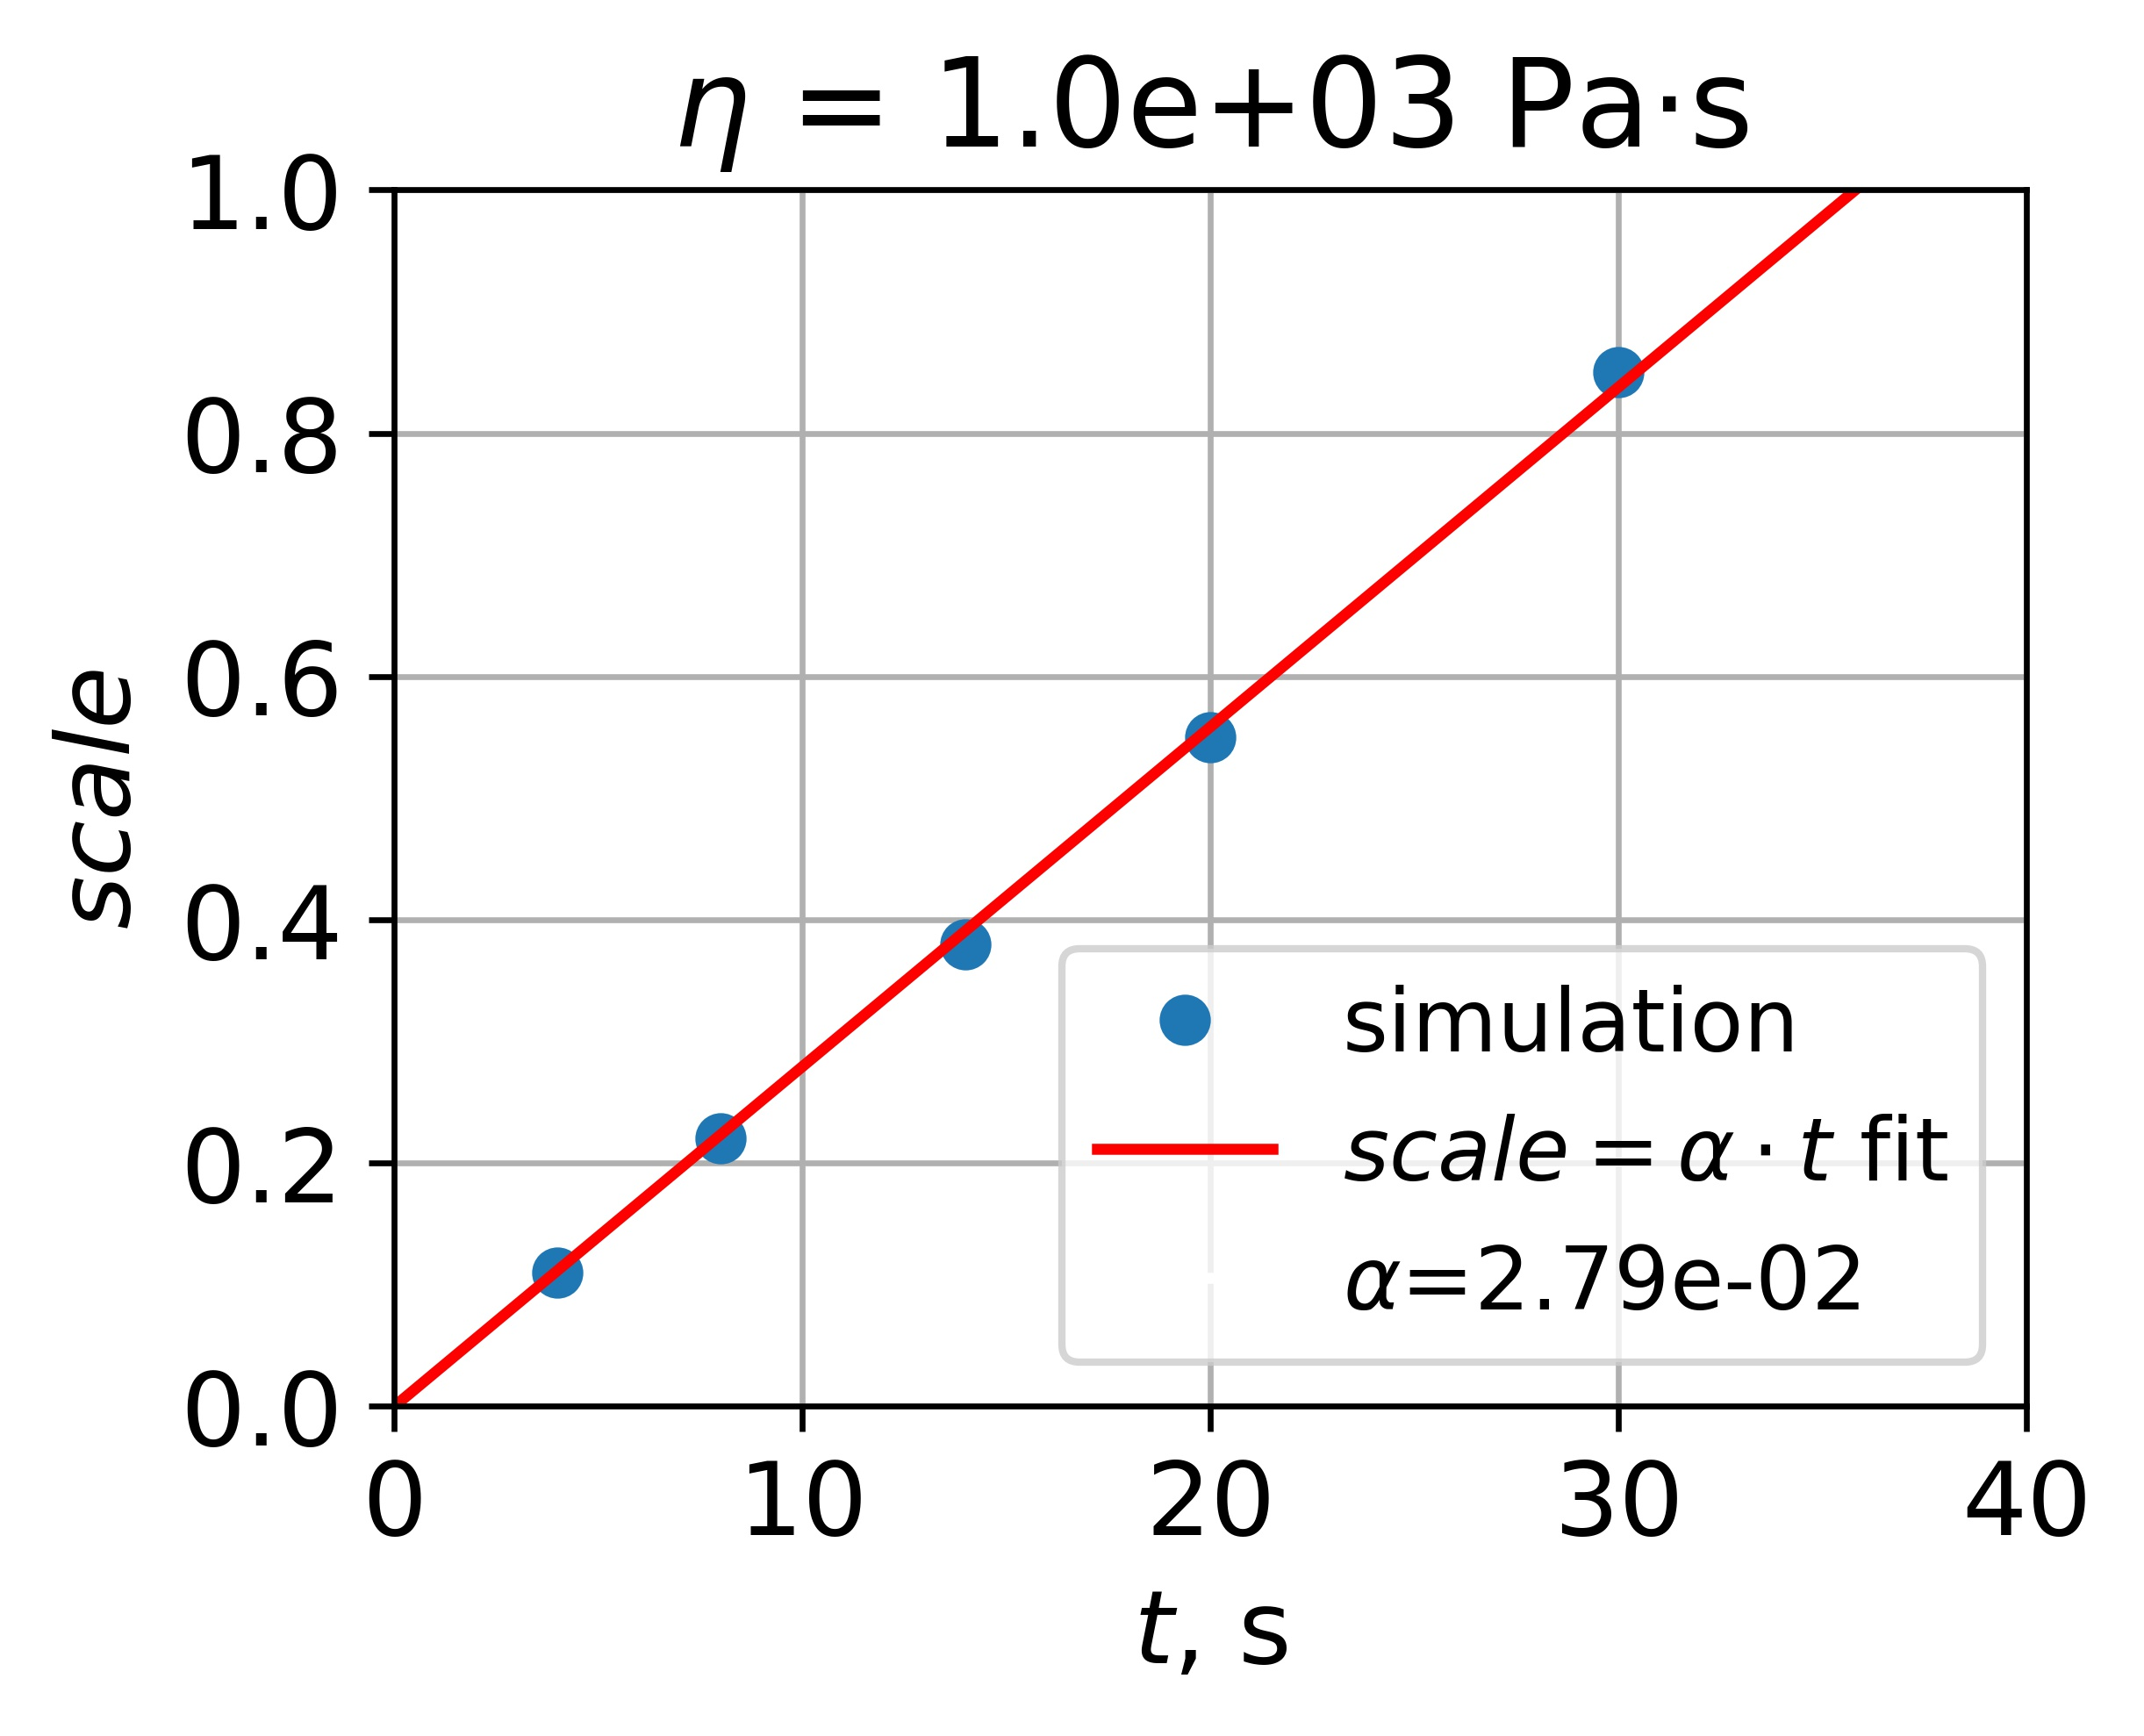
\includegraphics[width=\linewidth]{alpha_1000} \\
		\vspace{-13em} \\ \text{\hspace{-0.1em} b}) \\ \vspace{13em}
	\end{minipage}
	
	\vspace{-3em}
	
	\begin{minipage}{0.48\textwidth}
		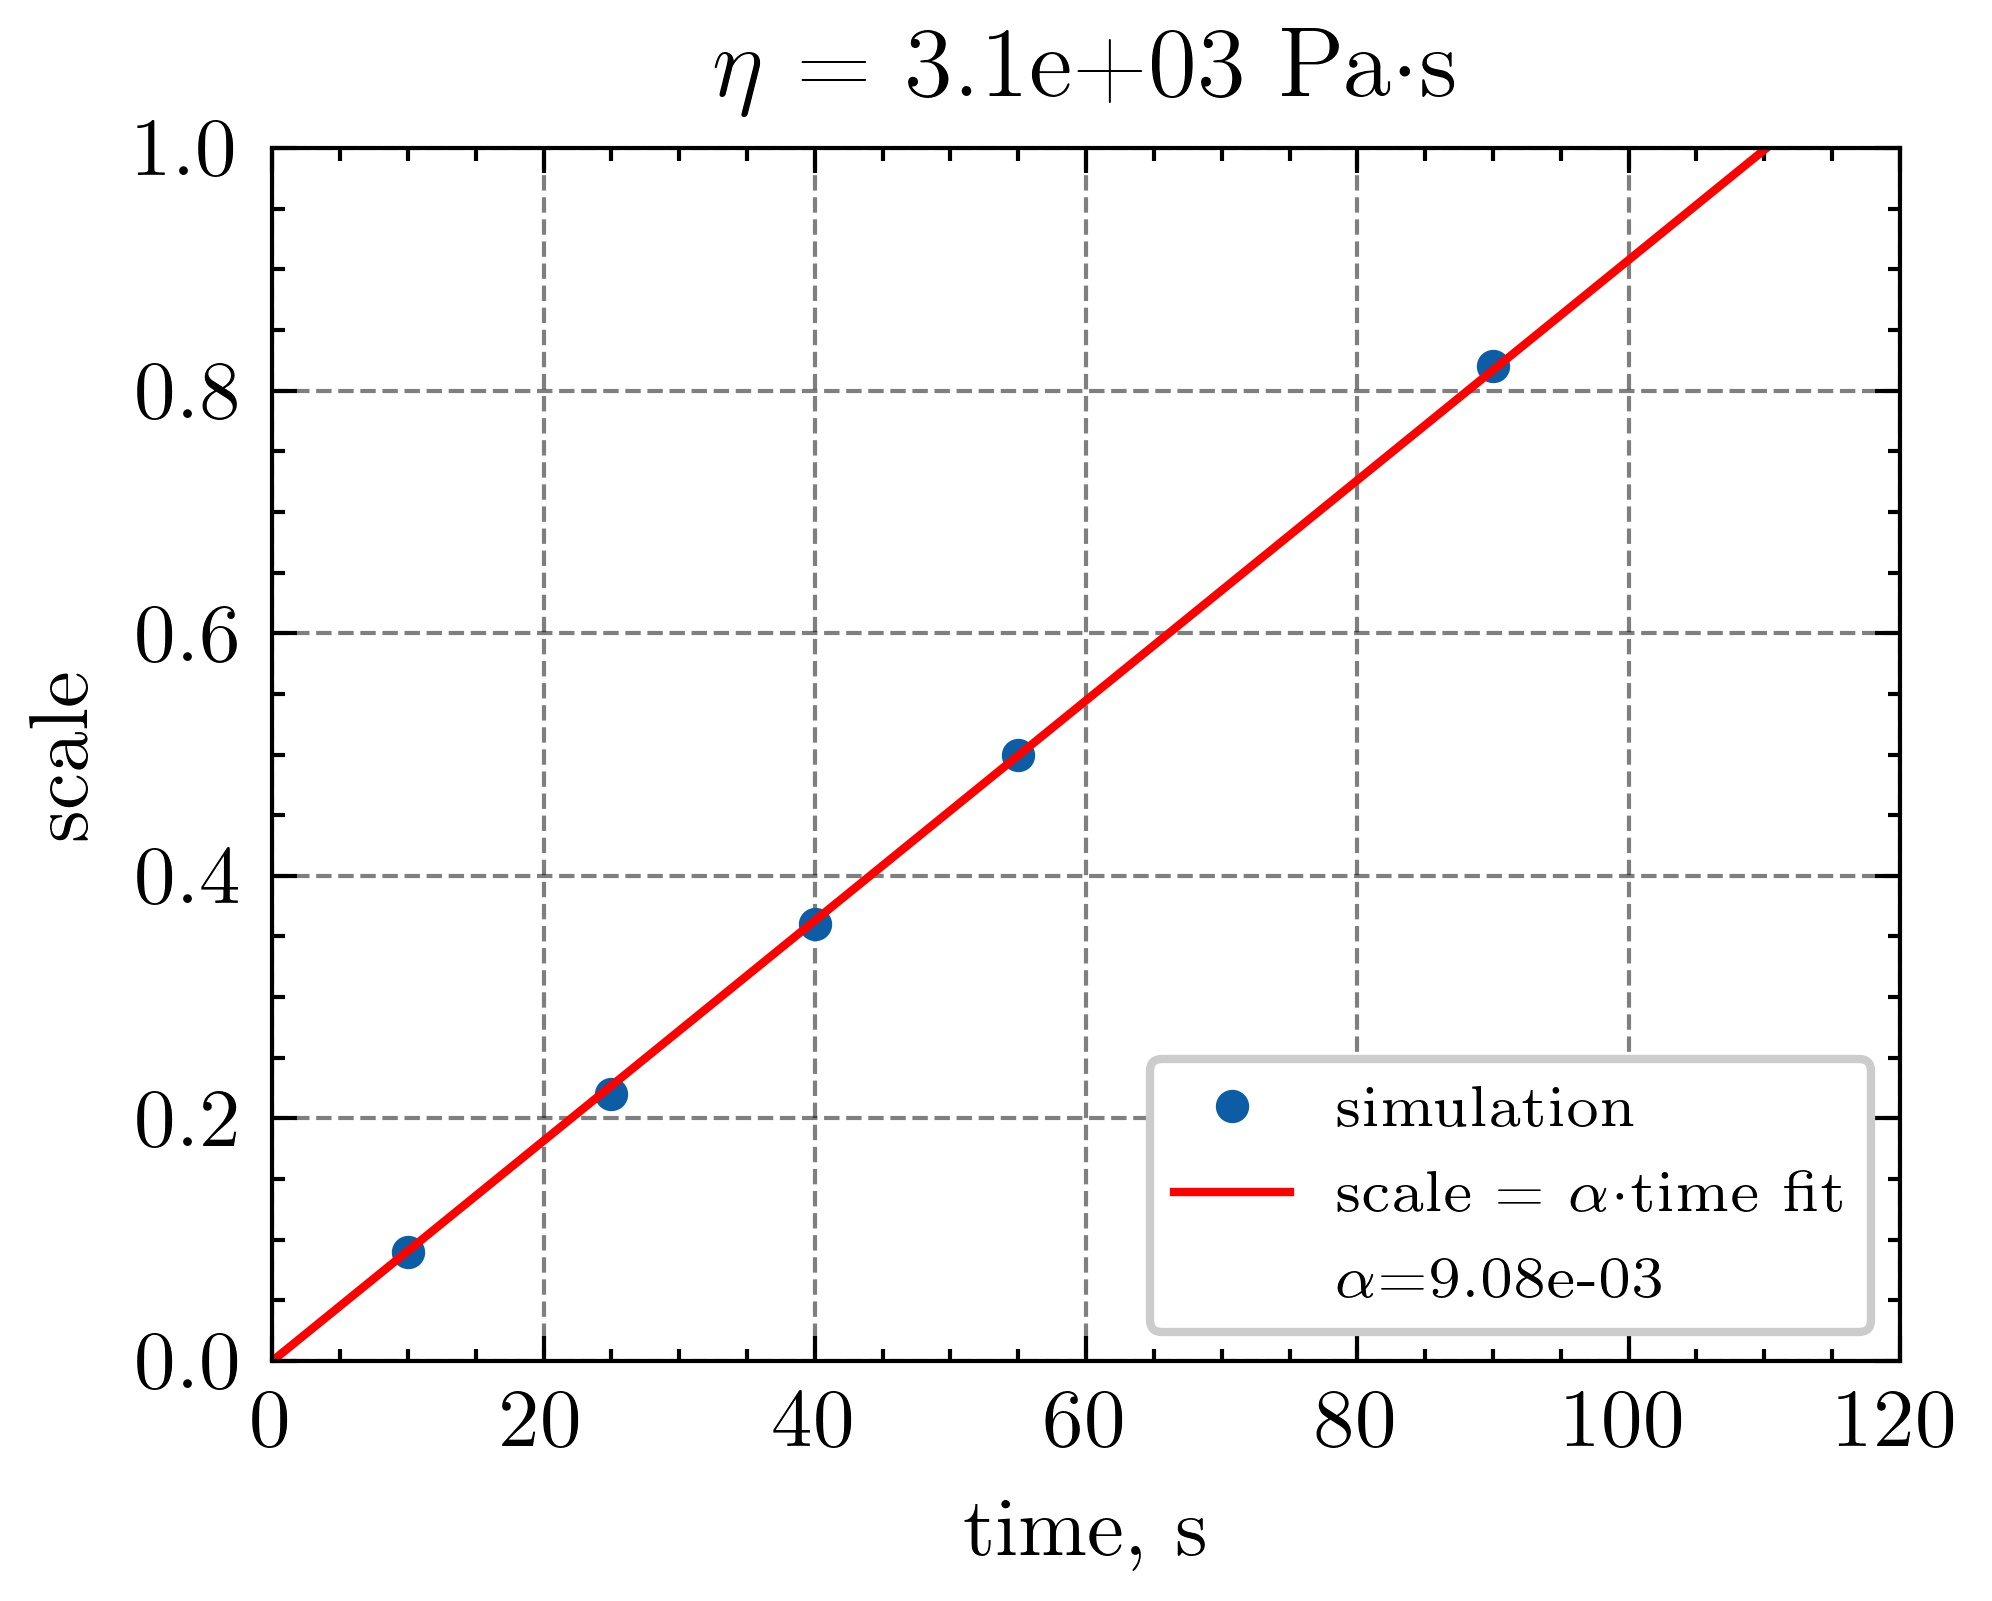
\includegraphics[width=\linewidth]{alpha_3100} \\
		\vspace{-13em} \\ \text{\hspace{0em} c}) \\ \vspace{13em}
	\end{minipage}
	\begin{minipage}{0.48\textwidth}
		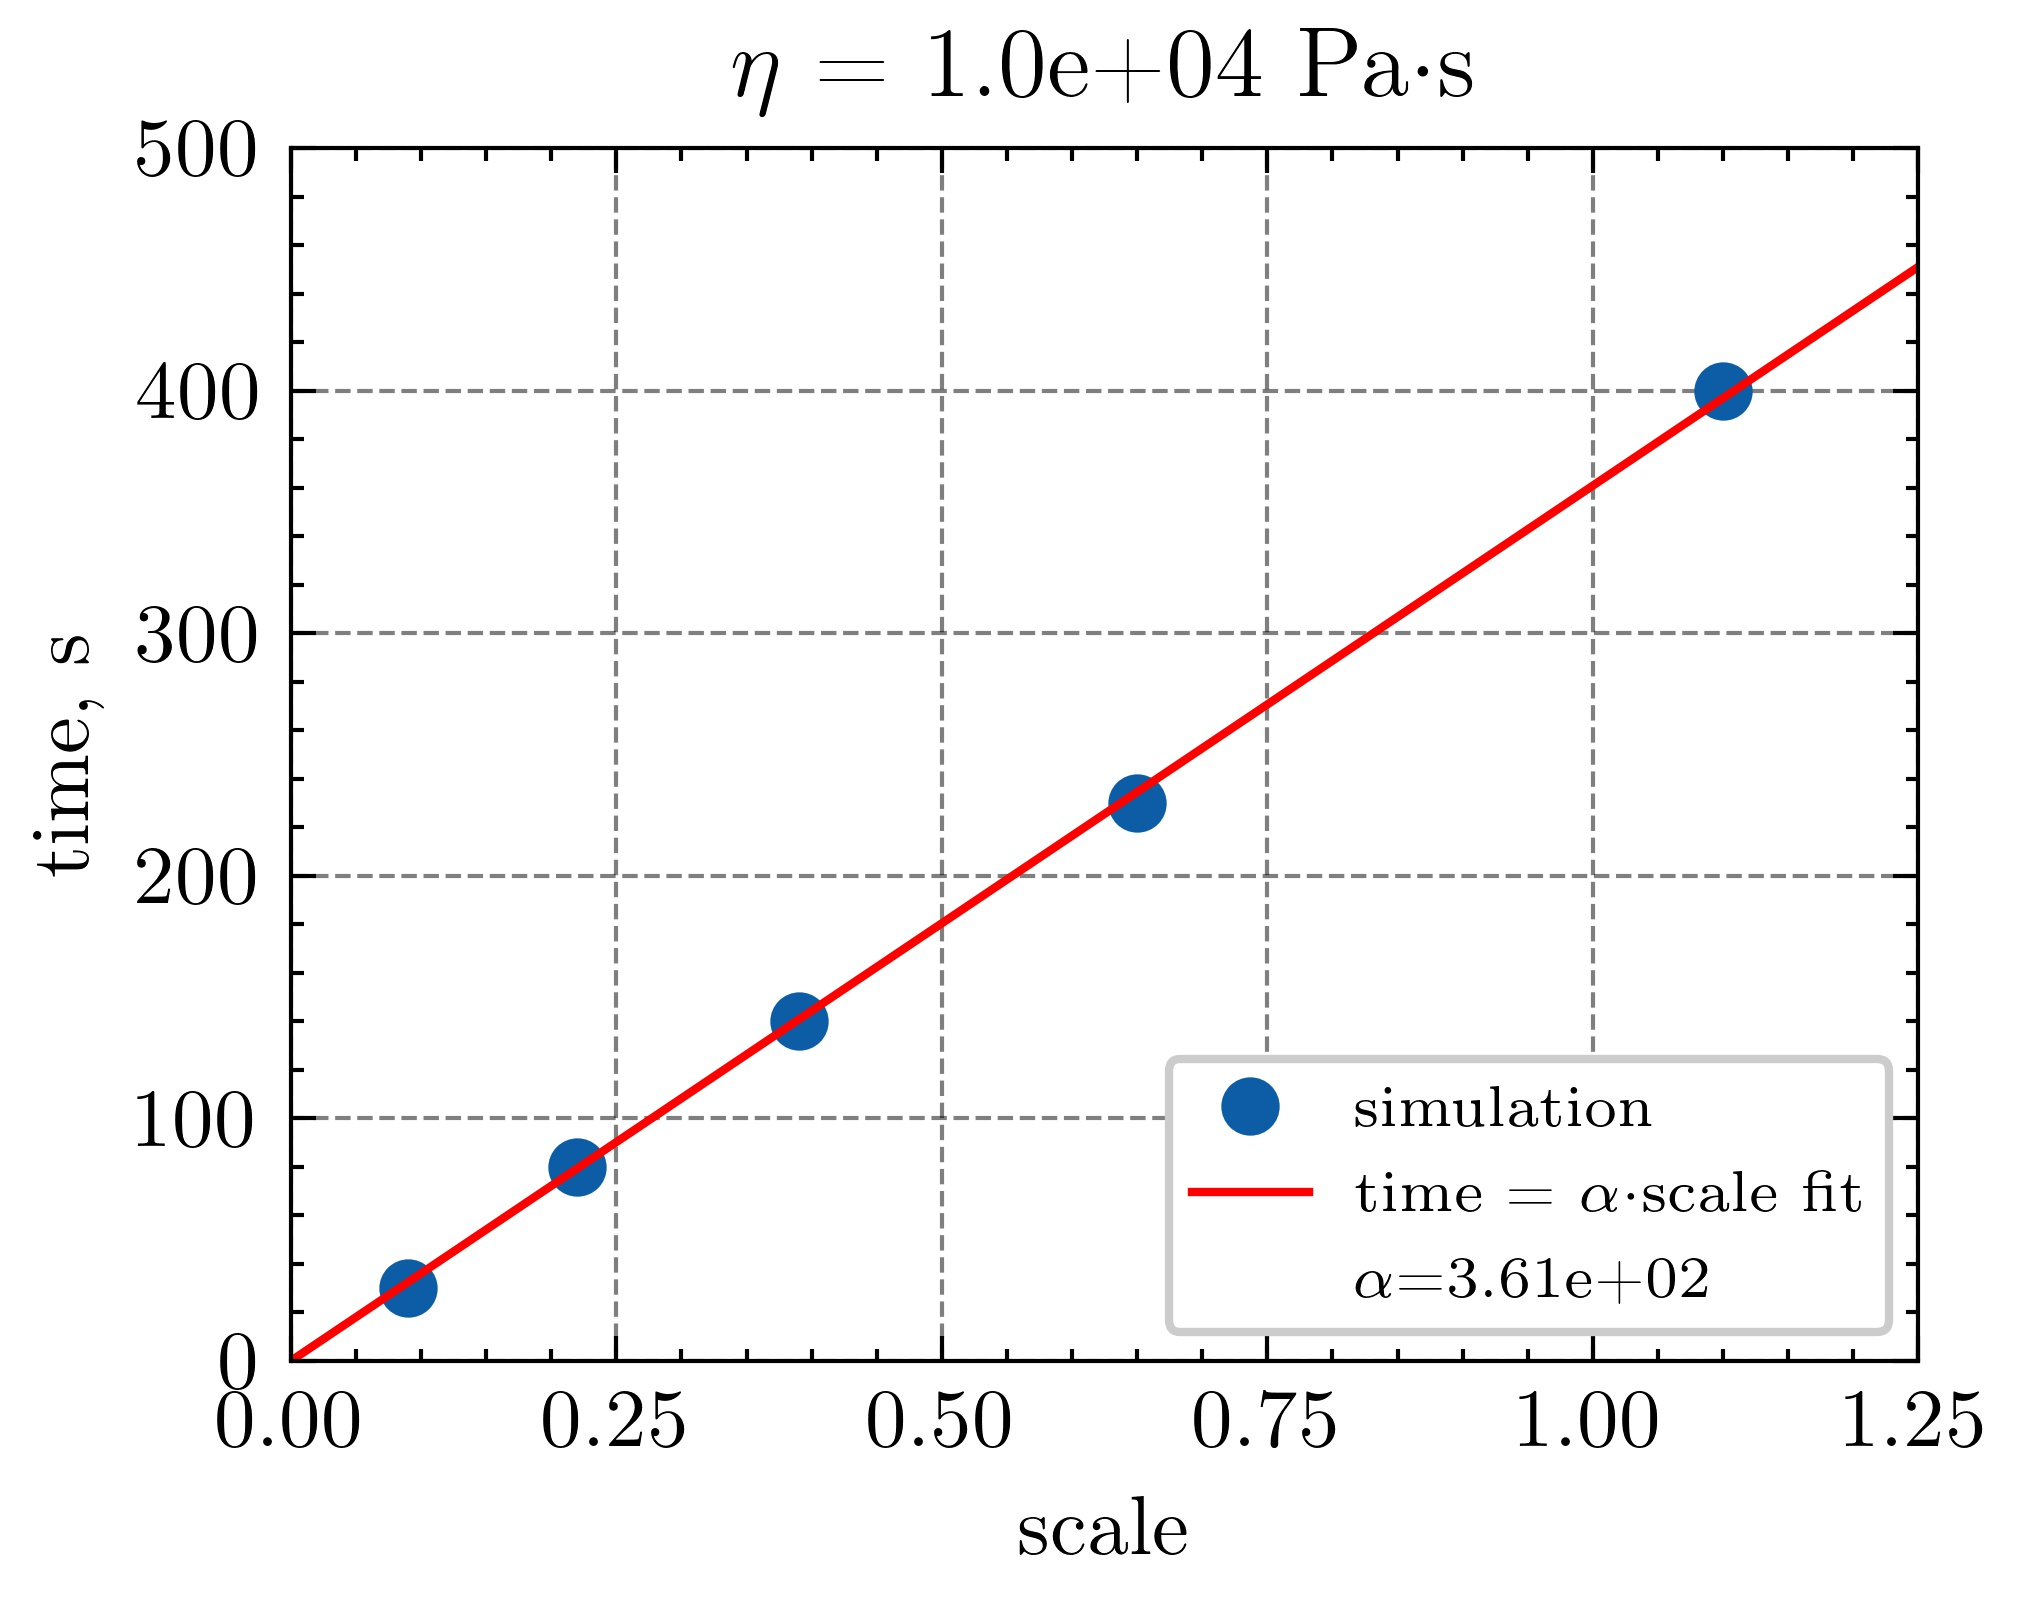
\includegraphics[width=\linewidth]{alpha_10000} \\
		\vspace{-13em} \\ \text{\hspace{-0.1em} d}) \\ \vspace{13em}
	\end{minipage}

	\vspace{-3em}
	
	\begin{minipage}{0.48\textwidth}
		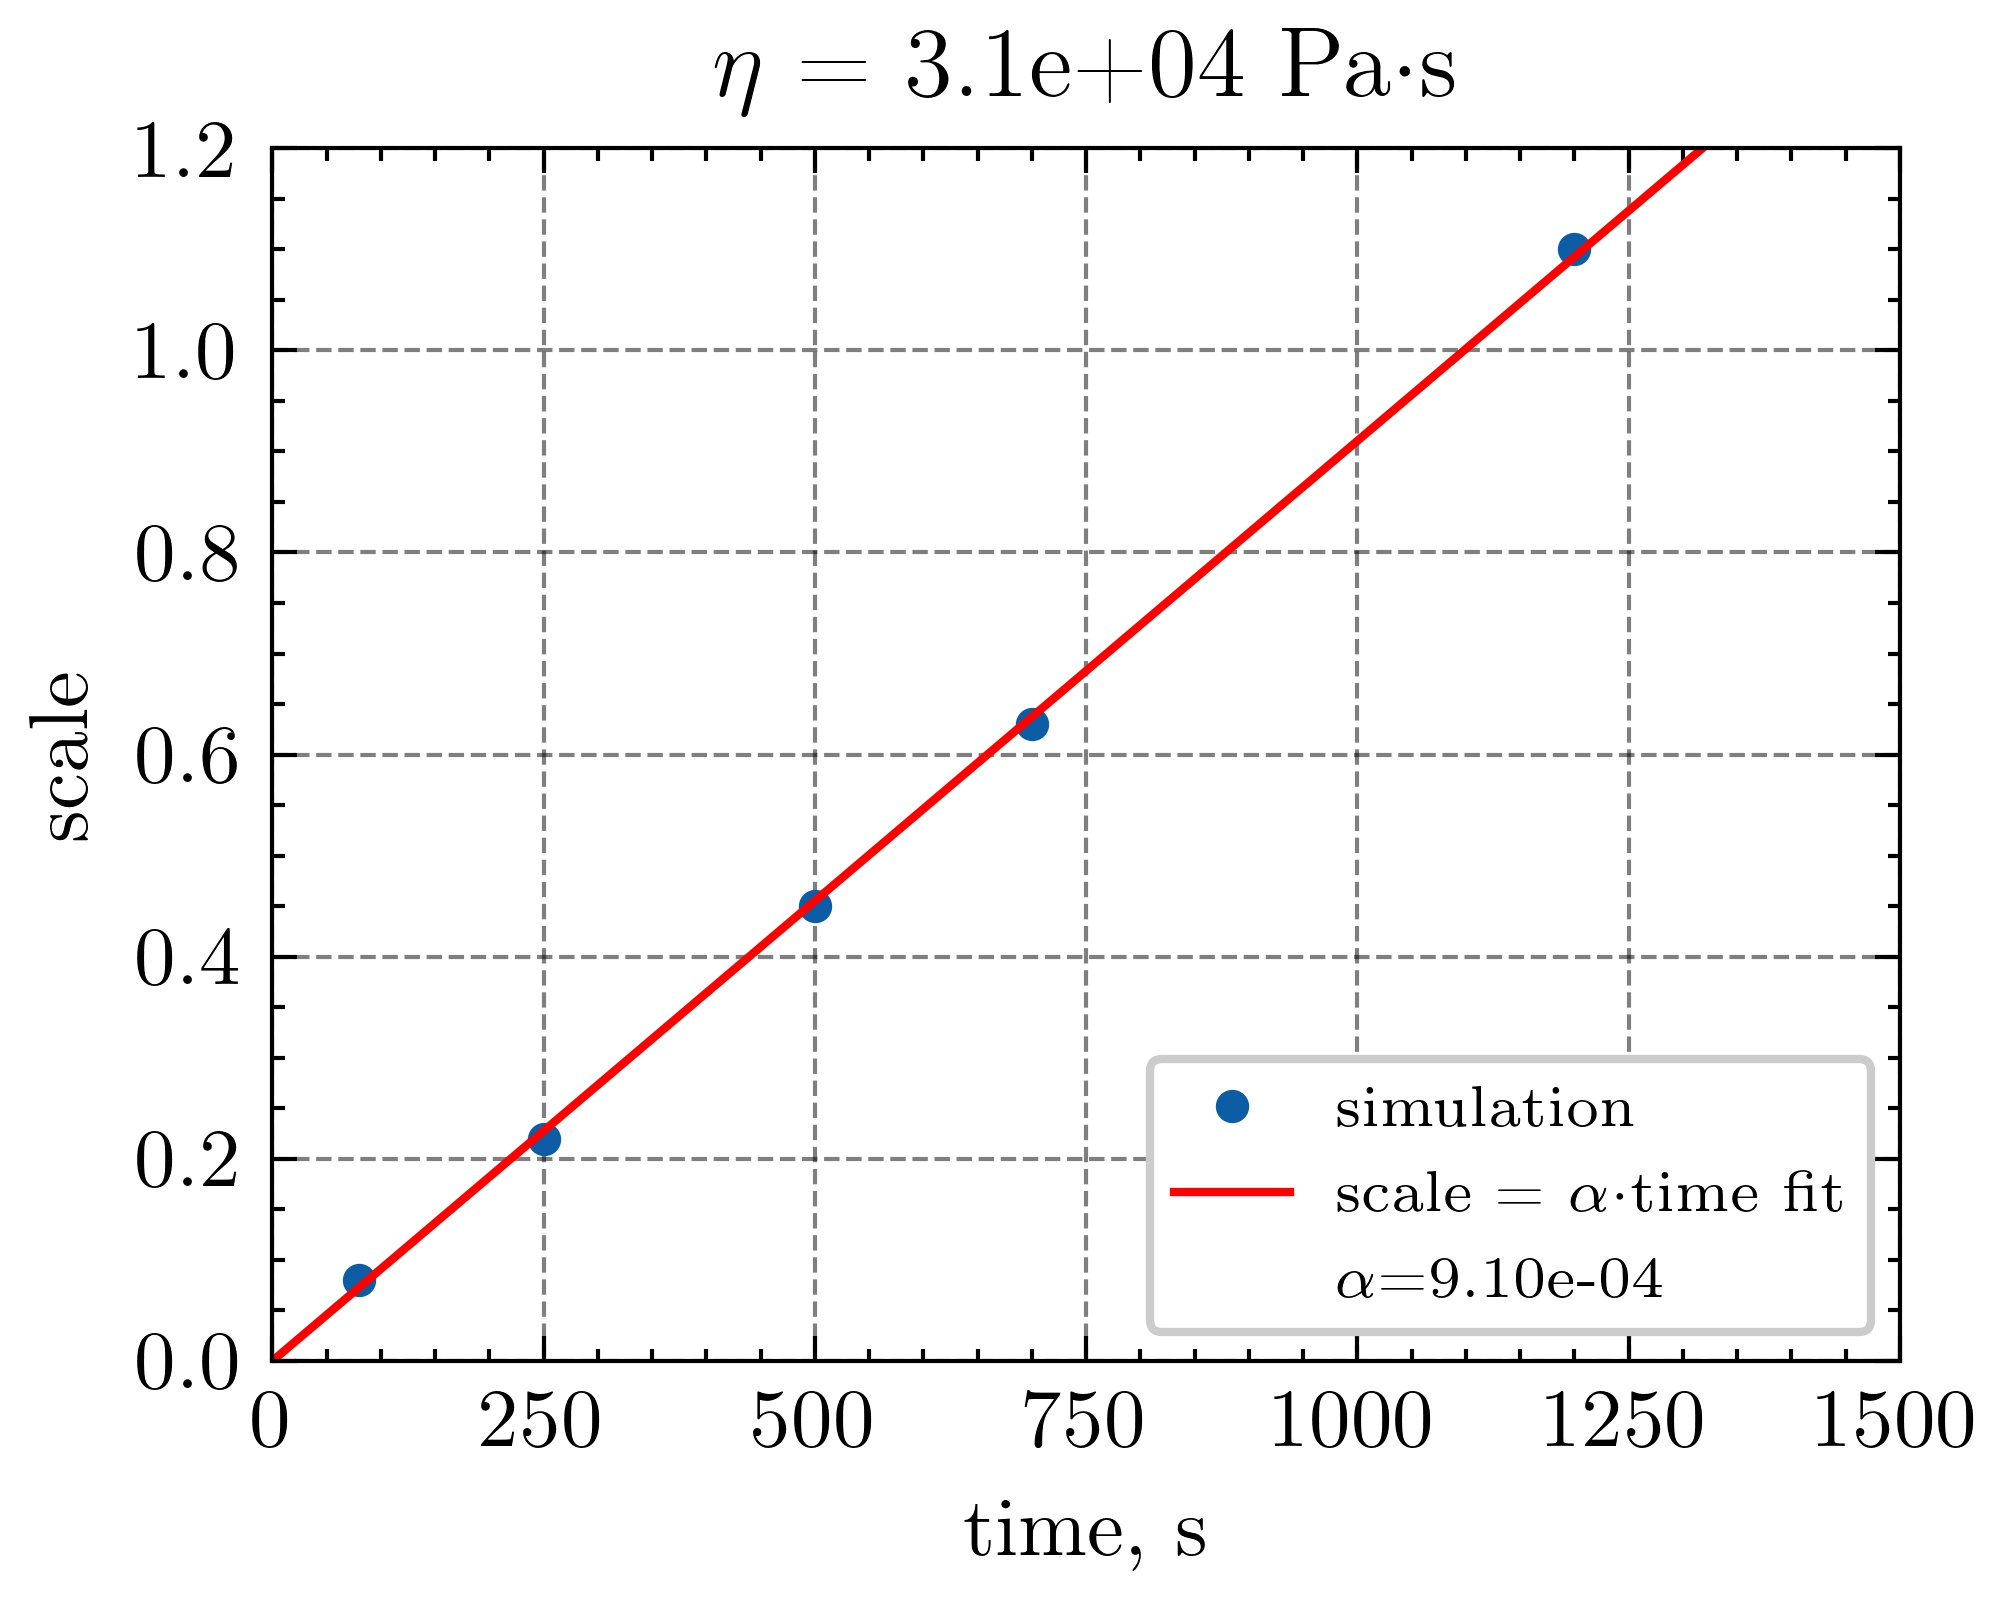
\includegraphics[width=\linewidth]{alpha_31000} \\
		\vspace{-13em} \\ \text{\hspace{0em} e}) \\ \vspace{13em}
	\end{minipage}
	\begin{minipage}{0.48\textwidth}
		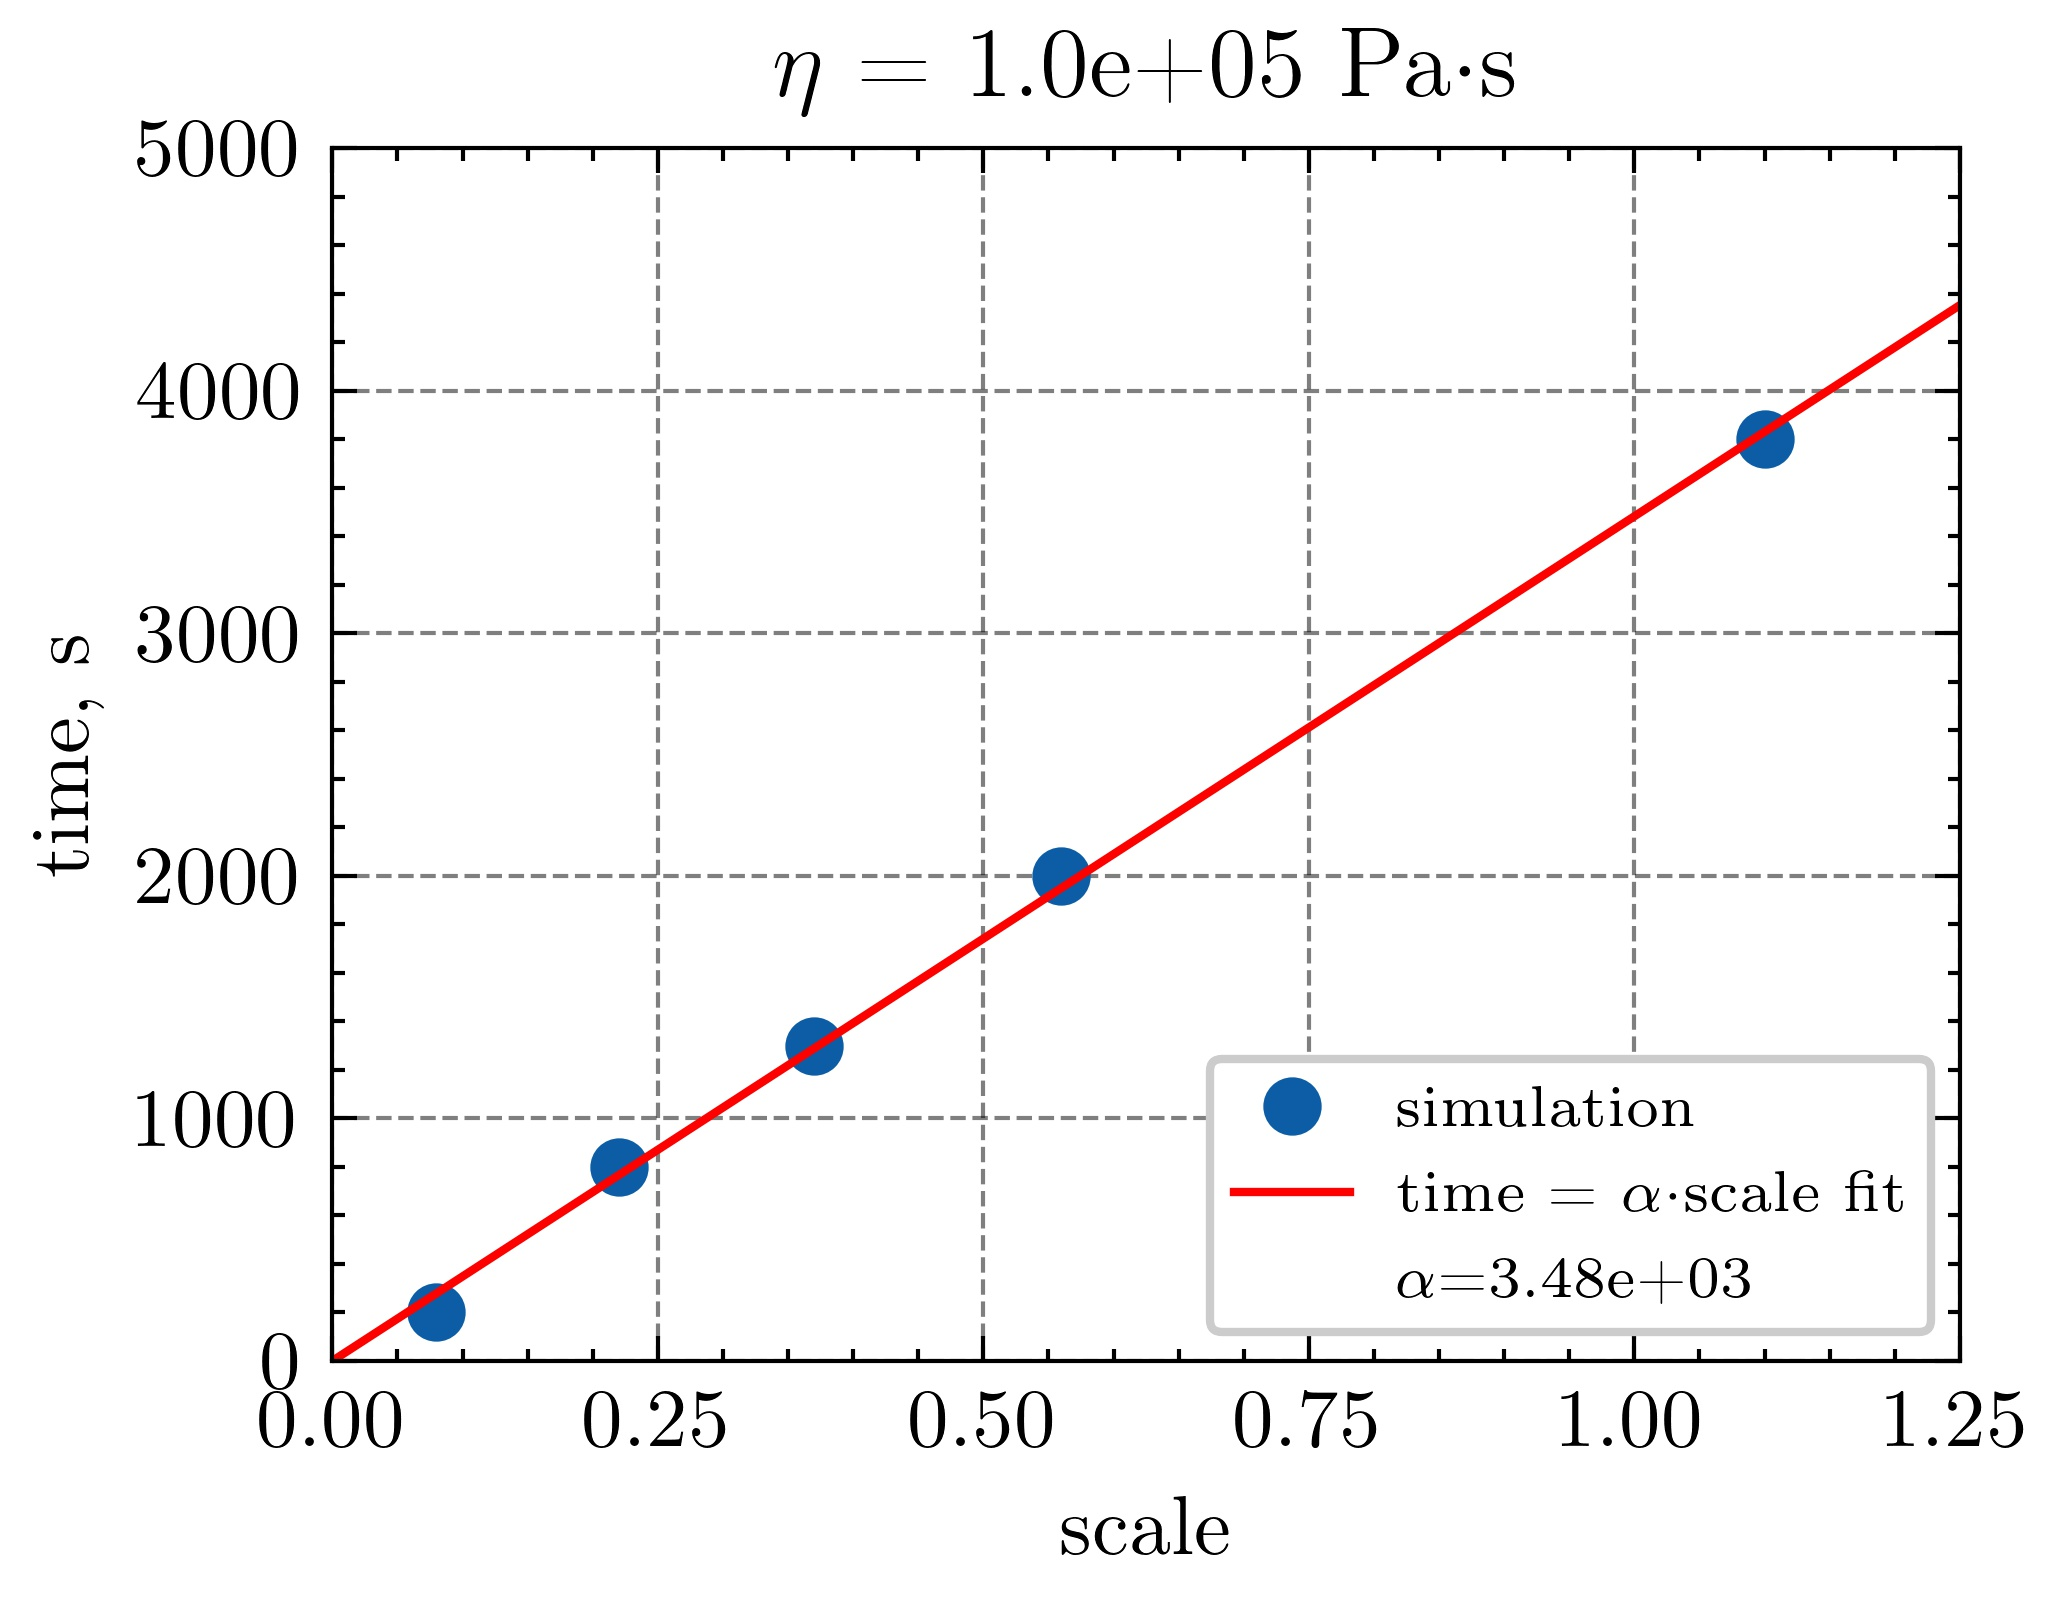
\includegraphics[width=\linewidth]{alpha_100000} \\
		\vspace{-13em} \\ \text{\hspace{-0.1em} f}) \\ \vspace{13em}
	\end{minipage}

	\vspace{-4em}

	\caption{Промоделированные периодические профили с периодом 3 мкм, полученные в слое ПММА с начальной толщиной 500 нм методом СЭЛТР при экспонировании по области с различным распределением плотности тока в пучке.}
	\label{fig:DEBER_multibeam}
\end{figure}

\begin{figure}
	\begin{center}
		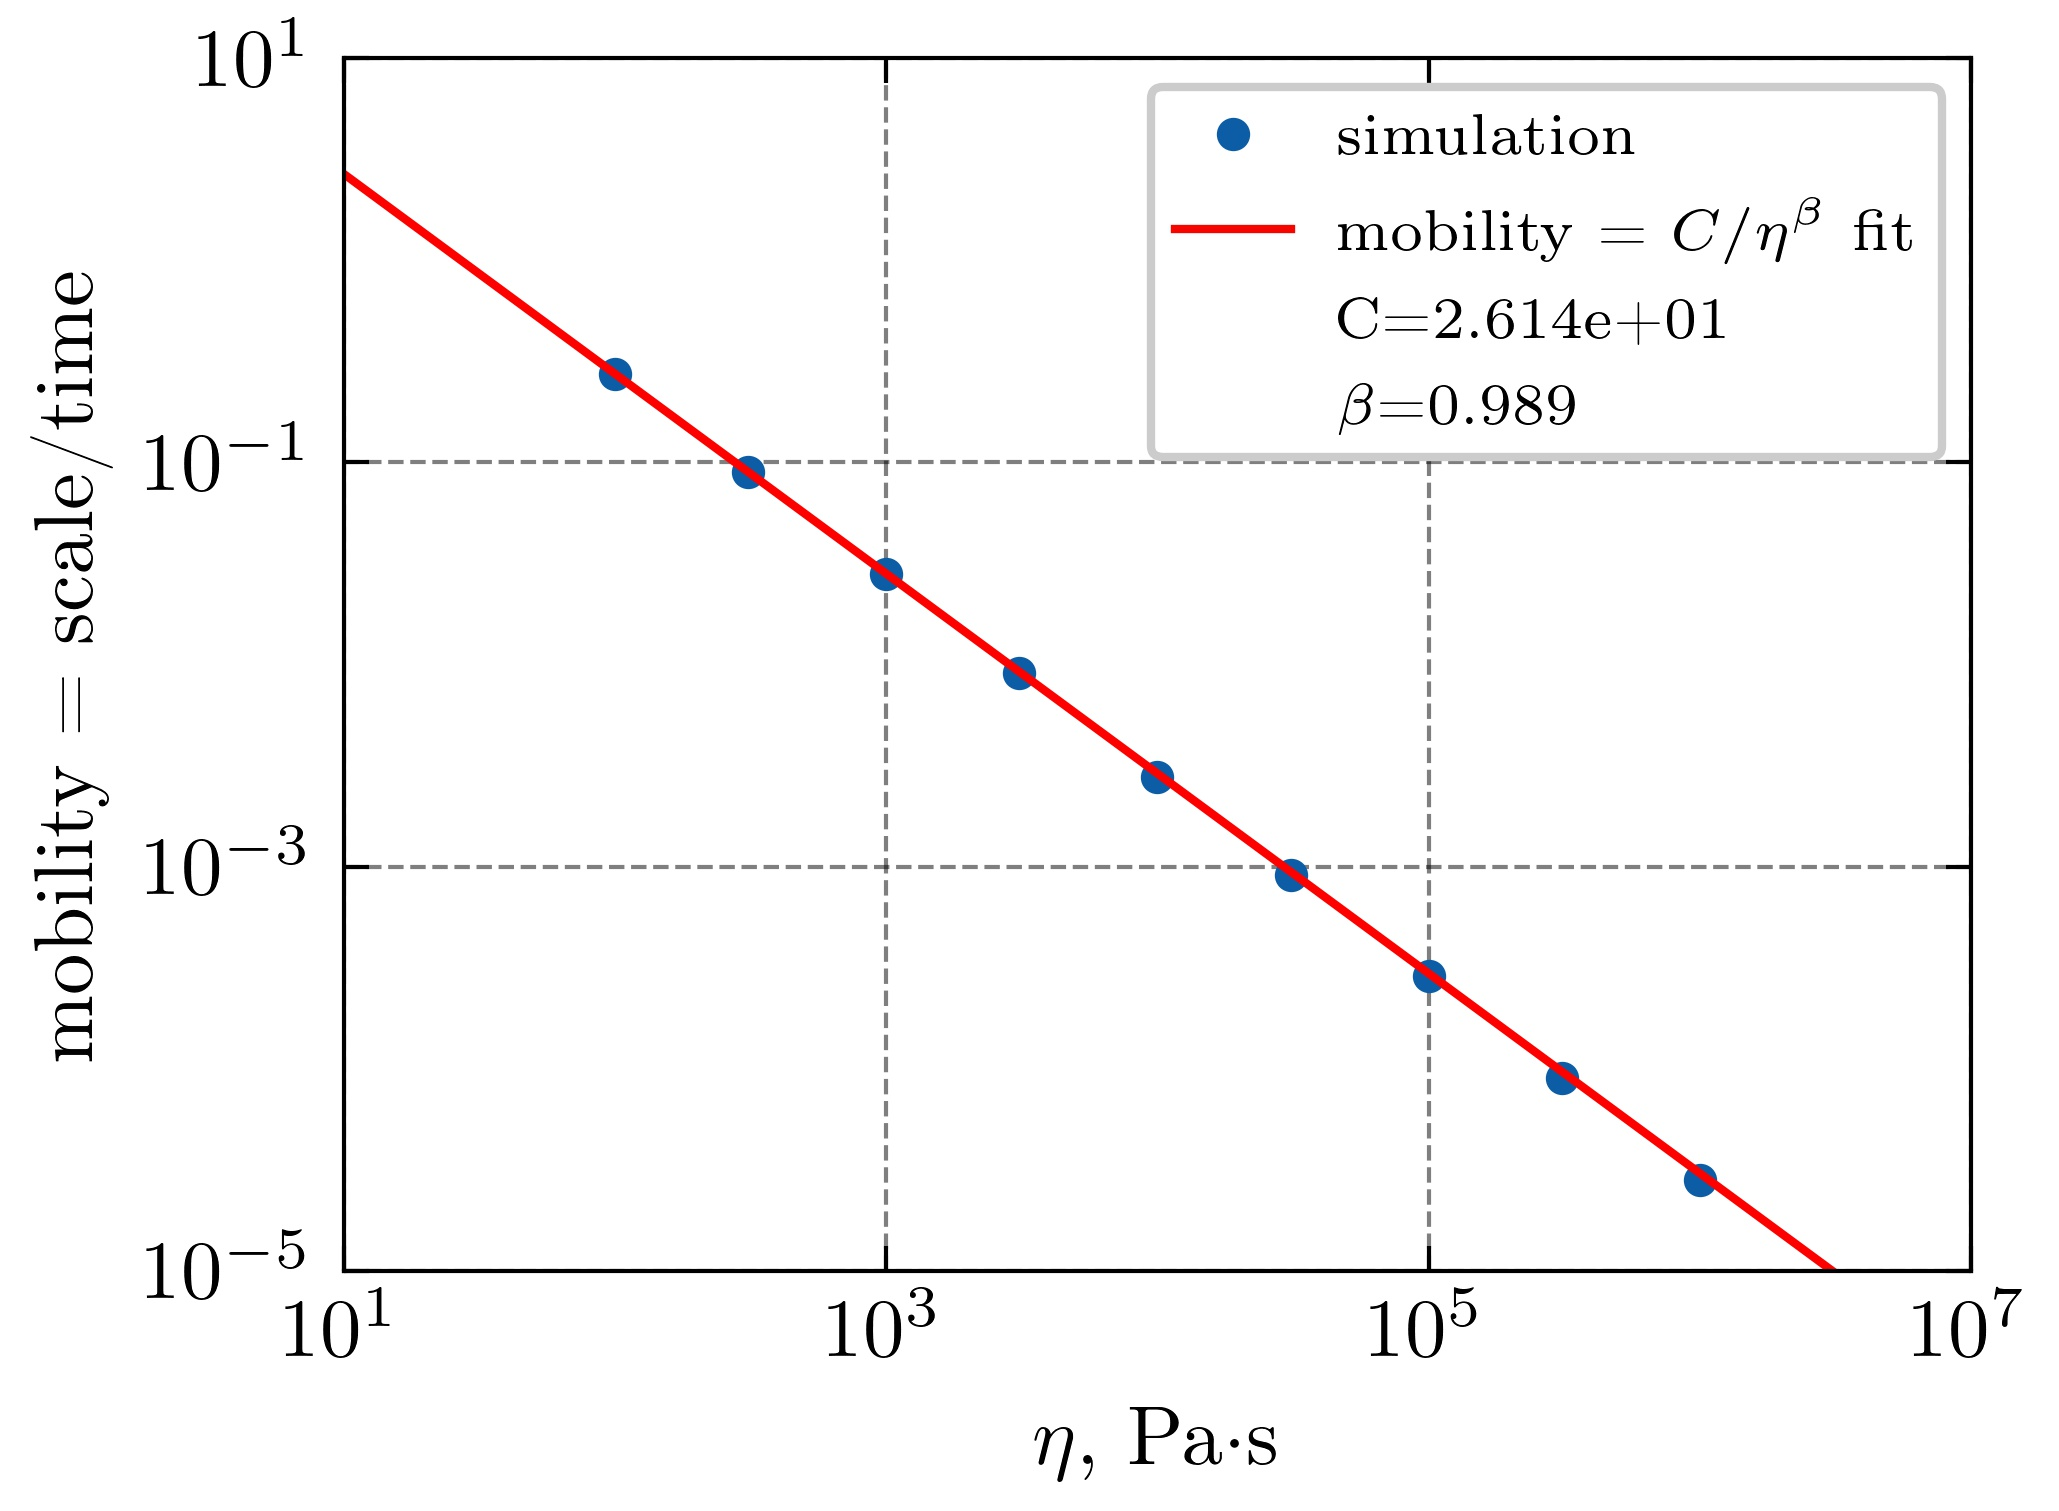
\includegraphics[width=0.6\linewidth]{final_fit}
	\end{center}
	
	\vspace{-2em}
	
	\caption{Промоделированные периодические профили с периодом 3 мкм, полученные в слое ПММА с начальной толщиной 500 нм методом СЭЛТР при экспонировании по области с различным распределением плотности тока в пучке. Темпера}
	\label{fig:DEBER_multibeam}
\end{figure}


\end{document}
